
At preselection, the expected SM processes in the \mumubj channel that are considered are \ZJETS, \ttbar, diboson, \TTV, single top, and \WJETS. The most dominant processes, \ZJETS, \ttbar, diboson, and \TTV are estimated with MC simulation and renormalized to data using high-purity control regions (CR). The remaining background processes---single top and \WJETS---are taken directly from MC simulation.

\subsection{\texorpdfstring{Estimation of \ZJETS, \ttbar, diboson, and \TTV backgrounds}{Estimation of Z/y* + jets, tt-bar, diboson, and ttV backgrounds}} \label{sec:BkgNorm}
The \ZJETS, \ttbar, diboson, and \TTV processes are modeled via the same approach: MC simulation is used to first estimate the background shape, then the background is normalized to data at preselection with scale factors extracted inside a high sample purity CR. The CR used for \ZJETS normalization is the \PZ-enriched mass window $80 < \Muu < \SI{100}{\GeV}$ (the \PZ mass-pole), referred to as region A. The \ZJETS normalization scale factors are also parameterized in bins of jet multiplicity. For normalizing \ttbar, a CR orthogonal to region A is used: the \ttbar-enriched mass window $100 < \Muu < \SI{100}{\GeV}$ (the top quark kinematic turn-on), referred to as region B. Diboson and \TTV backgrounds are normalized simultaneously in the same CR within the mass window $80 < \Muu < \SI{100}{\GeV}$, referred to as region C. While regions A and C share a mass window, region C also inverts the veto on a third lepton into a requirement that there are at least three leptons and is thus orthogonal to both regions A and B, and to retain sufficient statistics the b-jet tag requirement is dropped. The sample purity of the orthogonal regions A, B, and C were verified, being either \PZ-, \ttbar-, or \VV- and \TTV-enriched in the respective CRs. The normalization scale factors \RZ, \RTT, and \RVV are defined by:

\begin{equation}
       \RZ = \frac{\NCR{A}{Data} - \RTT\NCR{A}{\ttbar} - \NCR{A}{\VV} - \NCR{A}{\TTV} - \NCR{A}{O}}{\NCR{A}{\PZ}},
\end{equation}
\begin{equation}
       \RTT = \frac{\NCR{B}{Data} - \RZ\NCR{B}{\PZ} - \NCR{B}{\VV} - \NCR{B}{\TTV} - \NCR{B}{O}}{\NCR{B}{\ttbar}},
\end{equation}
and
\begin{equation}
       \RVV = \frac{\NCR{C}{Data} - \RZ\NCR{C}{\PZ} - \RTT\NCR{C}{\ttbar} - \NCR{C}{O}}{\NCR{C}{\VV} + \NCR{C}{\TTV}},
\end{equation}

where \Nevents{Data} is the number of data events, \Nevents{X} is the number of X-process SM background events, and \Nevents{O} is the number of events produced by ``other'' SM processes (i.e., single top and \WJETS), while the superscripts A, B, and C respectively denote the \PZ, \ttbar, and \VV/\TTV CRs from which these event counts are extracted. Due to the codependency of \RZ, \RTT, and \RVV, their values are initialized to unity, and the normalization factors are iteratively computed until the factors are stable. There is a strong dependence of the normalization scale factor in the \ZJETS background on the number of reconstructed jets, as seen in Fig.~\ref{fig:znjets}, so a jet-multiplicity-binned \ZJETS is used. The \ttbar background shows no such dependence. The scale factors and their uncertainties are listed for each year in Tables~\ref{tab:znormsf}-\ref{tab:vvnormsf}.

\begin{figure}[H]
       \centering
       {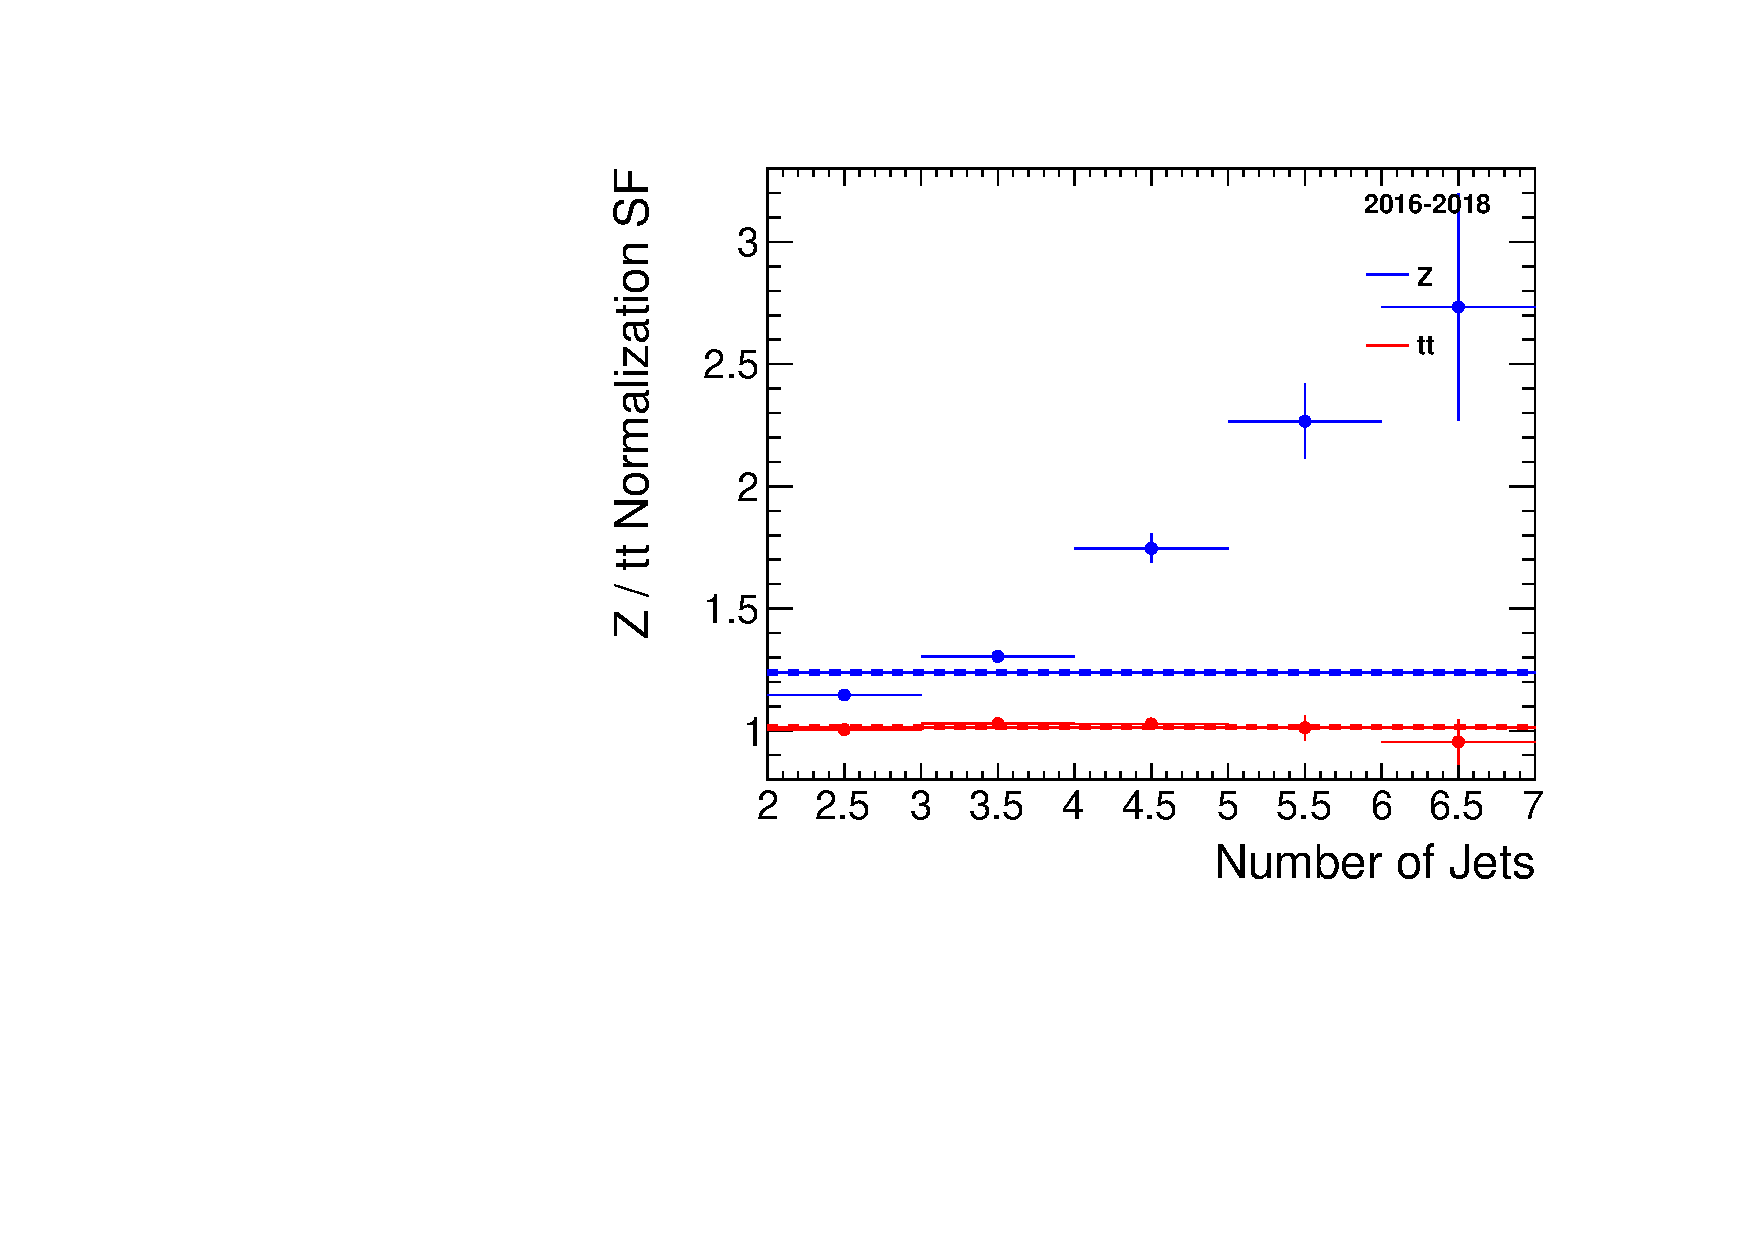
\includegraphics[width=\textwidth]{Images/Analysis/mumuScaleFactors_JetCount.pdf}}
       \caption{\ZJETS (blue) and \ttbar (red) normalization scale factors, in the full combined 2016-2018 dataset, binned in number of reconstructed jets. The horizontal dashed lines represent the inclusive scale factors.}
       \label{fig:znjets}
\end{figure}

\begin{table}[H]
       \caption{\ZJETS normalization scale factors by year.}
       \begin{center}
              %\scriptsize
              \begin{tabular}{ccccc}\hline\hline
                    Year & Control Region A [GeV] & \PZ Purity & \RZ & Jet Count\\ \hline
                    2016 & $80 < \Muu < 100$ & \SI{89}{\%} & $1.03 \pm 0.02$ \stat & 2\\
                    2016 & $80 < \Muu < 100$ & \SI{89}{\%} & $0.95 \pm 0.03$ \stat & 3\\
                    2016 & $80 < \Muu < 100$ & \SI{89}{\%} & $1.15 \pm 0.08$ \stat & 4\\
                    2016 & $80 < \Muu < 100$ & \SI{89}{\%} & $1.47 \pm 0.16$ \stat & $\geq5$\\
                    2017 & $80 < \Muu < 100$ & \SI{89}{\%} & $1.24 \pm 0.02$ \stat & 2\\
                    2017 & $80 < \Muu < 100$ & \SI{89}{\%} & $1.50 \pm 0.04$ \stat & 3\\
                    2017 & $80 < \Muu < 100$ & \SI{89}{\%} & $2.05 \pm 0.13$ \stat & 4\\
                    2017 & $80 < \Muu < 100$ & \SI{89}{\%} & $2.82 \pm 0.35$ \stat & $\geq5$\\
                    2018 & $80 < \Muu < 100$ & \SI{88}{\%} & $1.16 \pm 0.02$ \stat & 2\\ 
                    2018 & $80 < \Muu < 100$ & \SI{88}{\%} & $1.44 \pm 0.04$ \stat & 3\\ 
                    2018 & $80 < \Muu < 100$ & \SI{88}{\%} & $2.02 \pm 0.11$ \stat & 4\\ 
                    2018 & $80 < \Muu < 100$ & \SI{88}{\%} & $2.80 \pm 0.34$ \stat & $\geq5$\\ \hline\hline
              \end{tabular}
              \label{tab:znormsf}
       \end{center}
\end{table}

\begin{table}[H]
       \caption{\ttbar normalization scale factors by year.}
       \begin{center}
              %\scriptsize
              \begin{tabular}{cccc}\hline\hline
                    Year & Control Region B [GeV] & \ttbar Purity & \RTT \\ \hline
                    2016 & $100 < \Muu < 250$ & \SI{87}{\%} \% & $0.99 \pm 0.01$ \stat \\
                    2017 & $100 < \Muu < 250$ & \SI{89}{\%} \% & $1.09 \pm 0.01$ \stat \\
                    2018 & $100 < \Muu < 250$ & \SI{88}{\%} \% & $0.98 \pm 0.01$ \stat \\ \hline\hline
              \end{tabular}
              \label{tab:ttnormsf}
       \end{center}
\end{table}

\begin{table}[H]
       \caption{\VV and \TTV normalization scale factors by year.}
       \begin{center}
              %\scriptsize
              \begin{tabular}{cccccc}\hline\hline
                    Year & Control Region C [GeV] & Lepton Count & b-Jet Count & \VV + \TTV Purity & \RVV \\ \hline
                    2016 & $80 < \Muu < 100$ & $\geq 3$ & $\geq 0$  & \SI{80}{\%} & $1.1 \pm 0.1$ \stat \\
                    2017 & $80 < \Muu < 100$ & $\geq 3$ & $\geq 0$  & \SI{80}{\%} & $1.2 \pm 0.1$ \stat \\
                    2018 & $80 < \Muu < 100$ & $\geq 3$ & $\geq 0$  & \SI{80}{\%} & $1.4 \pm 0.1$ \stat \\ \hline\hline
              \end{tabular}
              \label{tab:vvnormsf}
       \end{center}
\end{table}

Studies on the stability of the background normalization scale factors can be found in Appendix~\ref{app:SFStudy}.

Observed and expected \Muu distributions at preselection are shown in Figs.~\ref{figapp:preselmasszoom} and~\ref{figapp:preselmasszoomcombined} that are zoomed into the respective CRs. Two representative signal MC samples are shown as well, with the normalization described in Section~\ref{sec:SimSignal}.

\begin{figure}[H]
    \centering
    {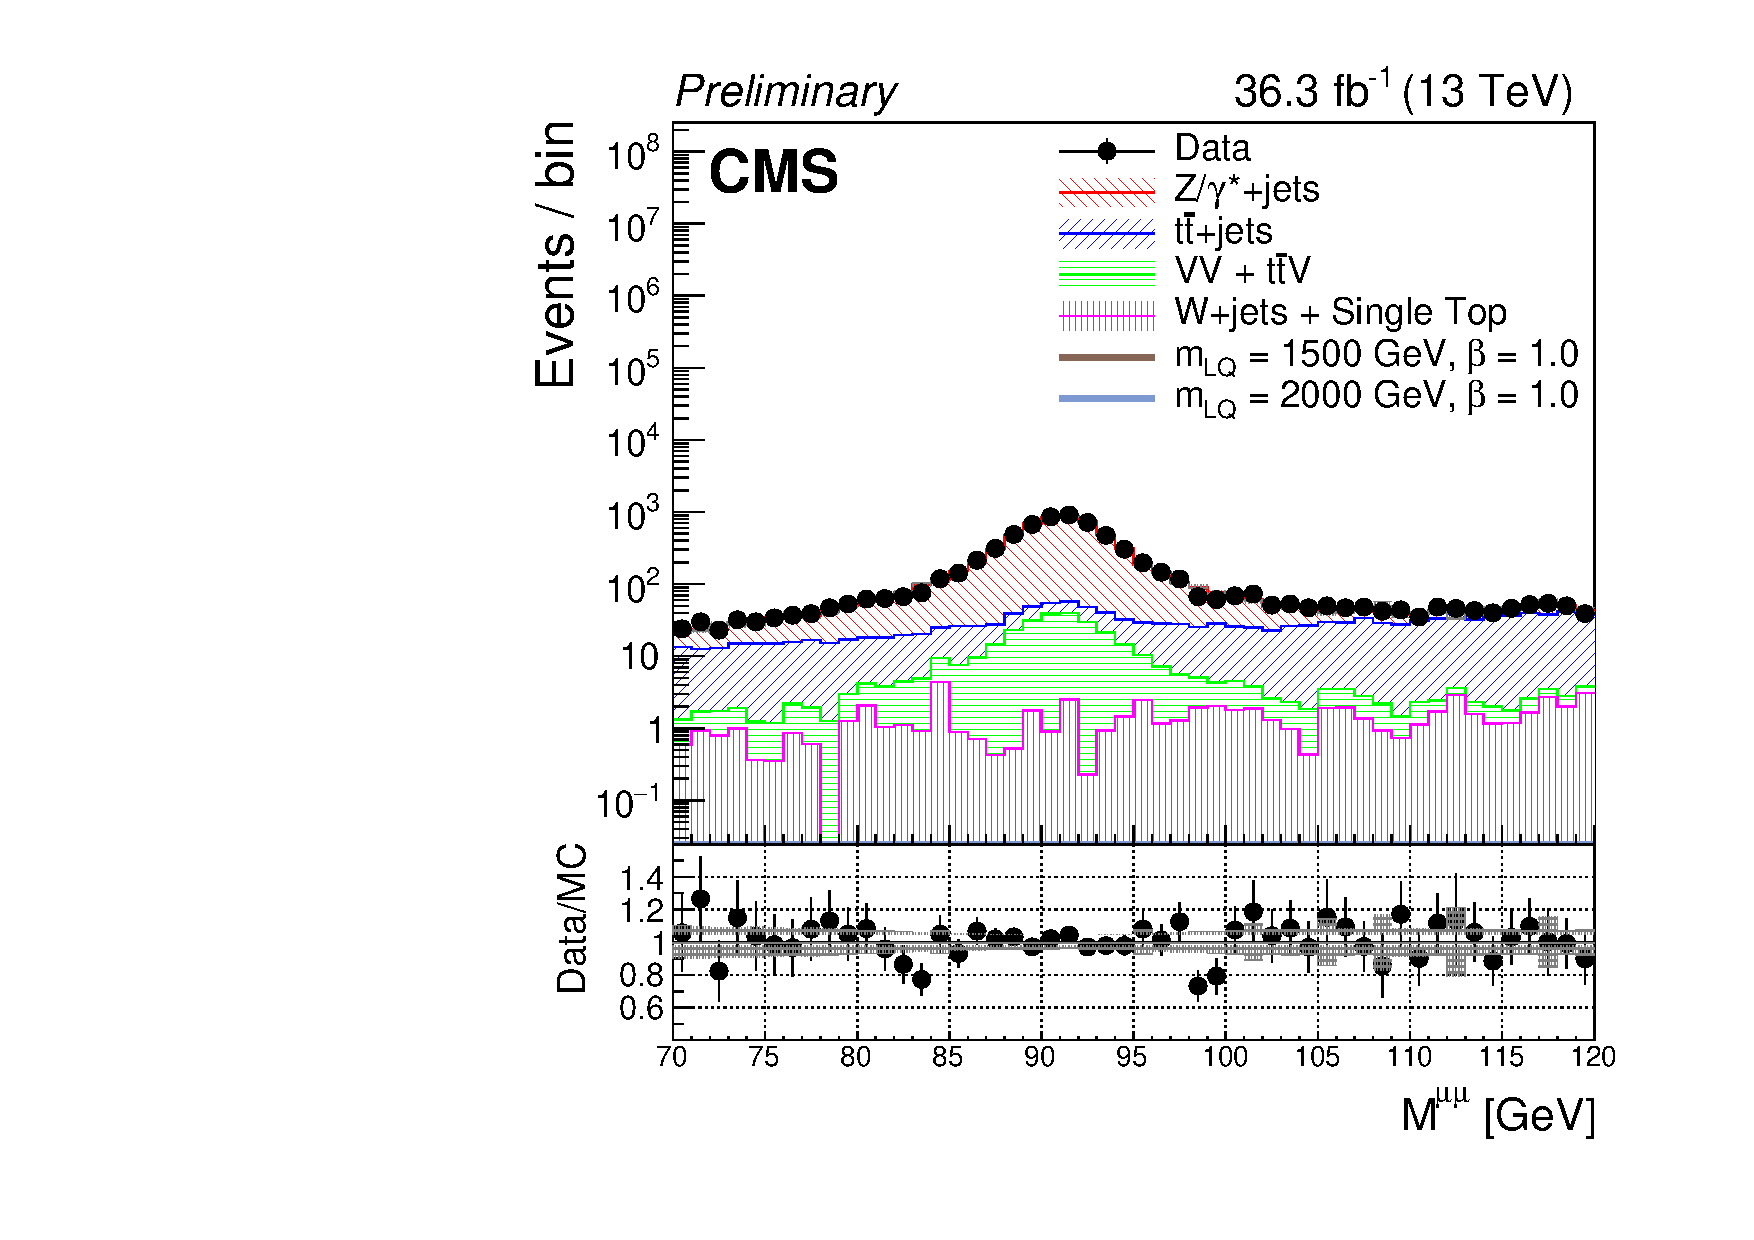
\includegraphics[width=.32\textwidth]{Images/Analysis/Results_2016_Unblinded/Plots/Preselection/BasicLQ_uujj_M_uu_controlzoom_ZRegion.pdf}}
    {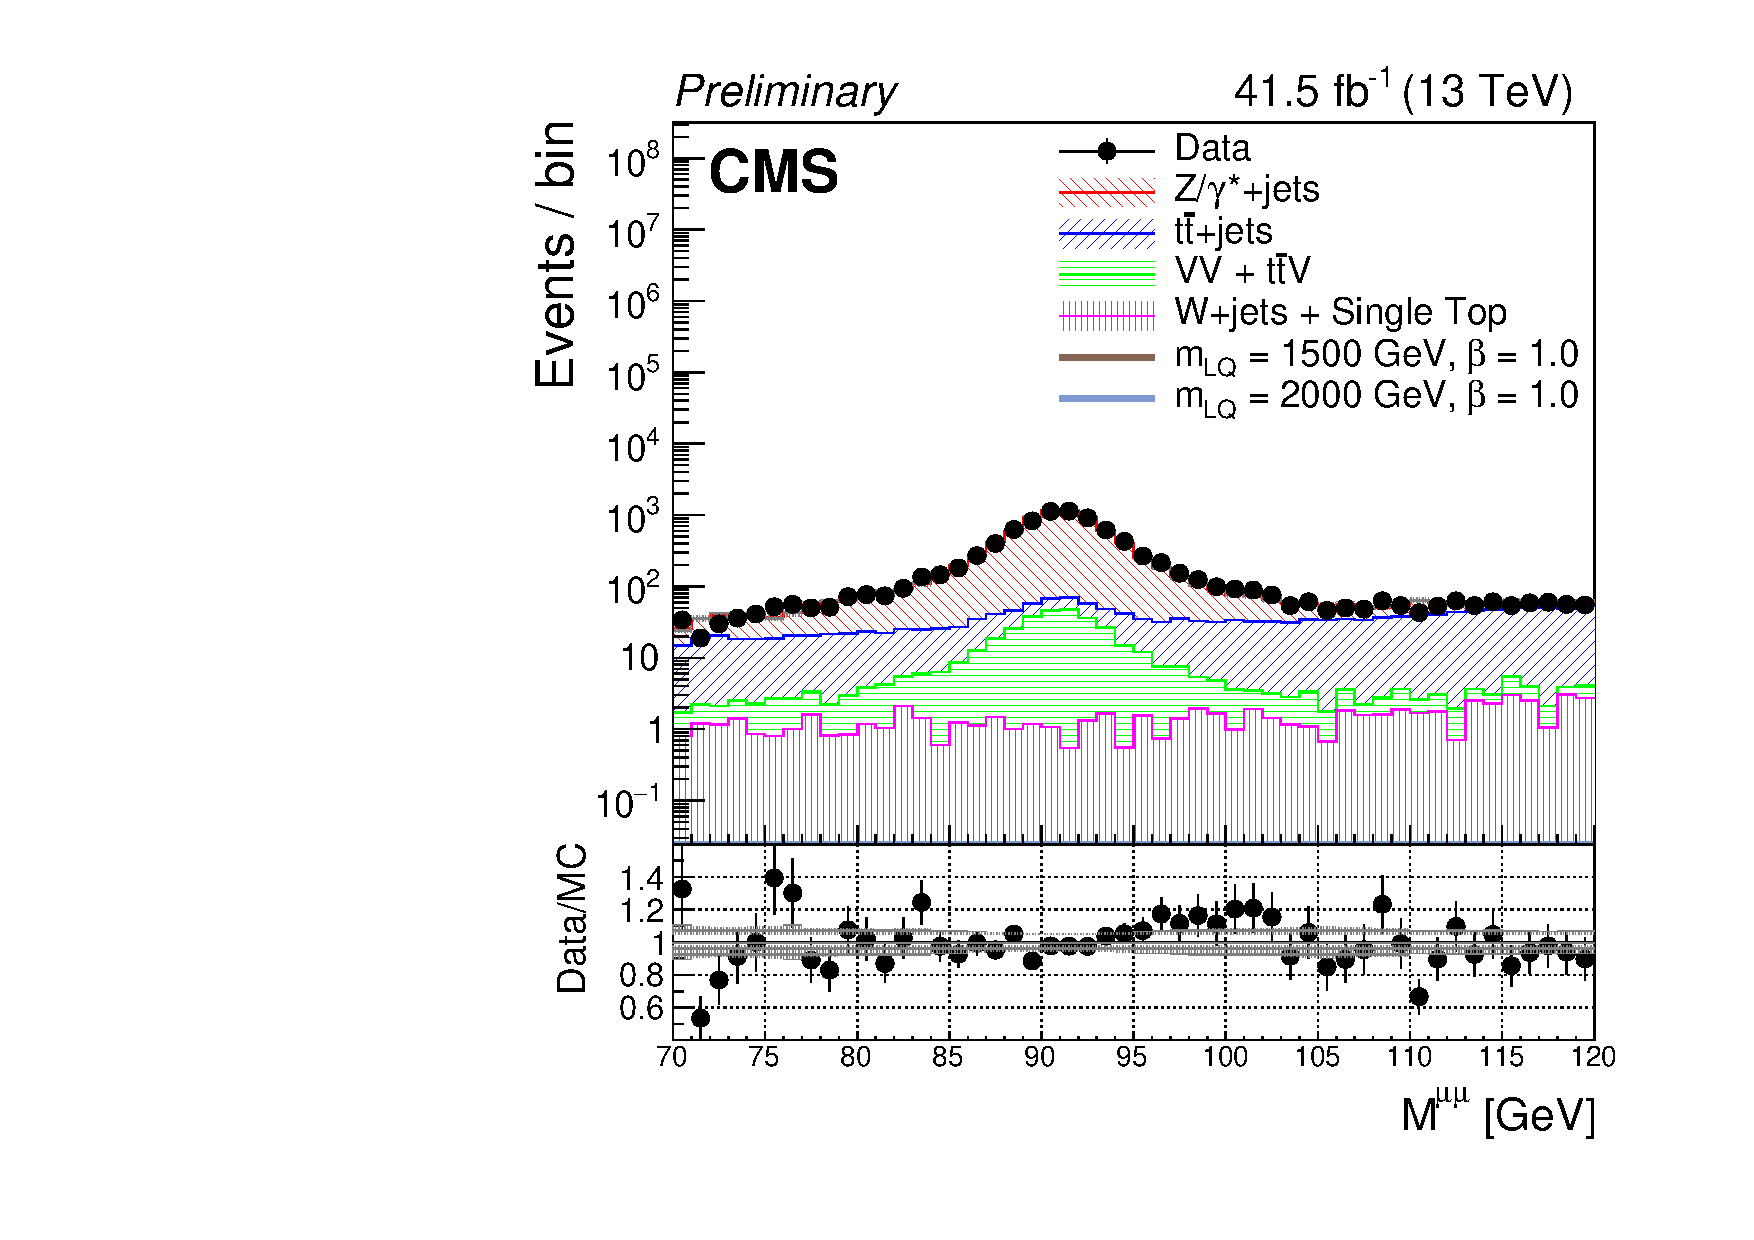
\includegraphics[width=.32\textwidth]{Images/Analysis/Results_2017_Unblinded/Plots/Preselection/BasicLQ_uujj_M_uu_controlzoom_ZRegion.pdf}}
    {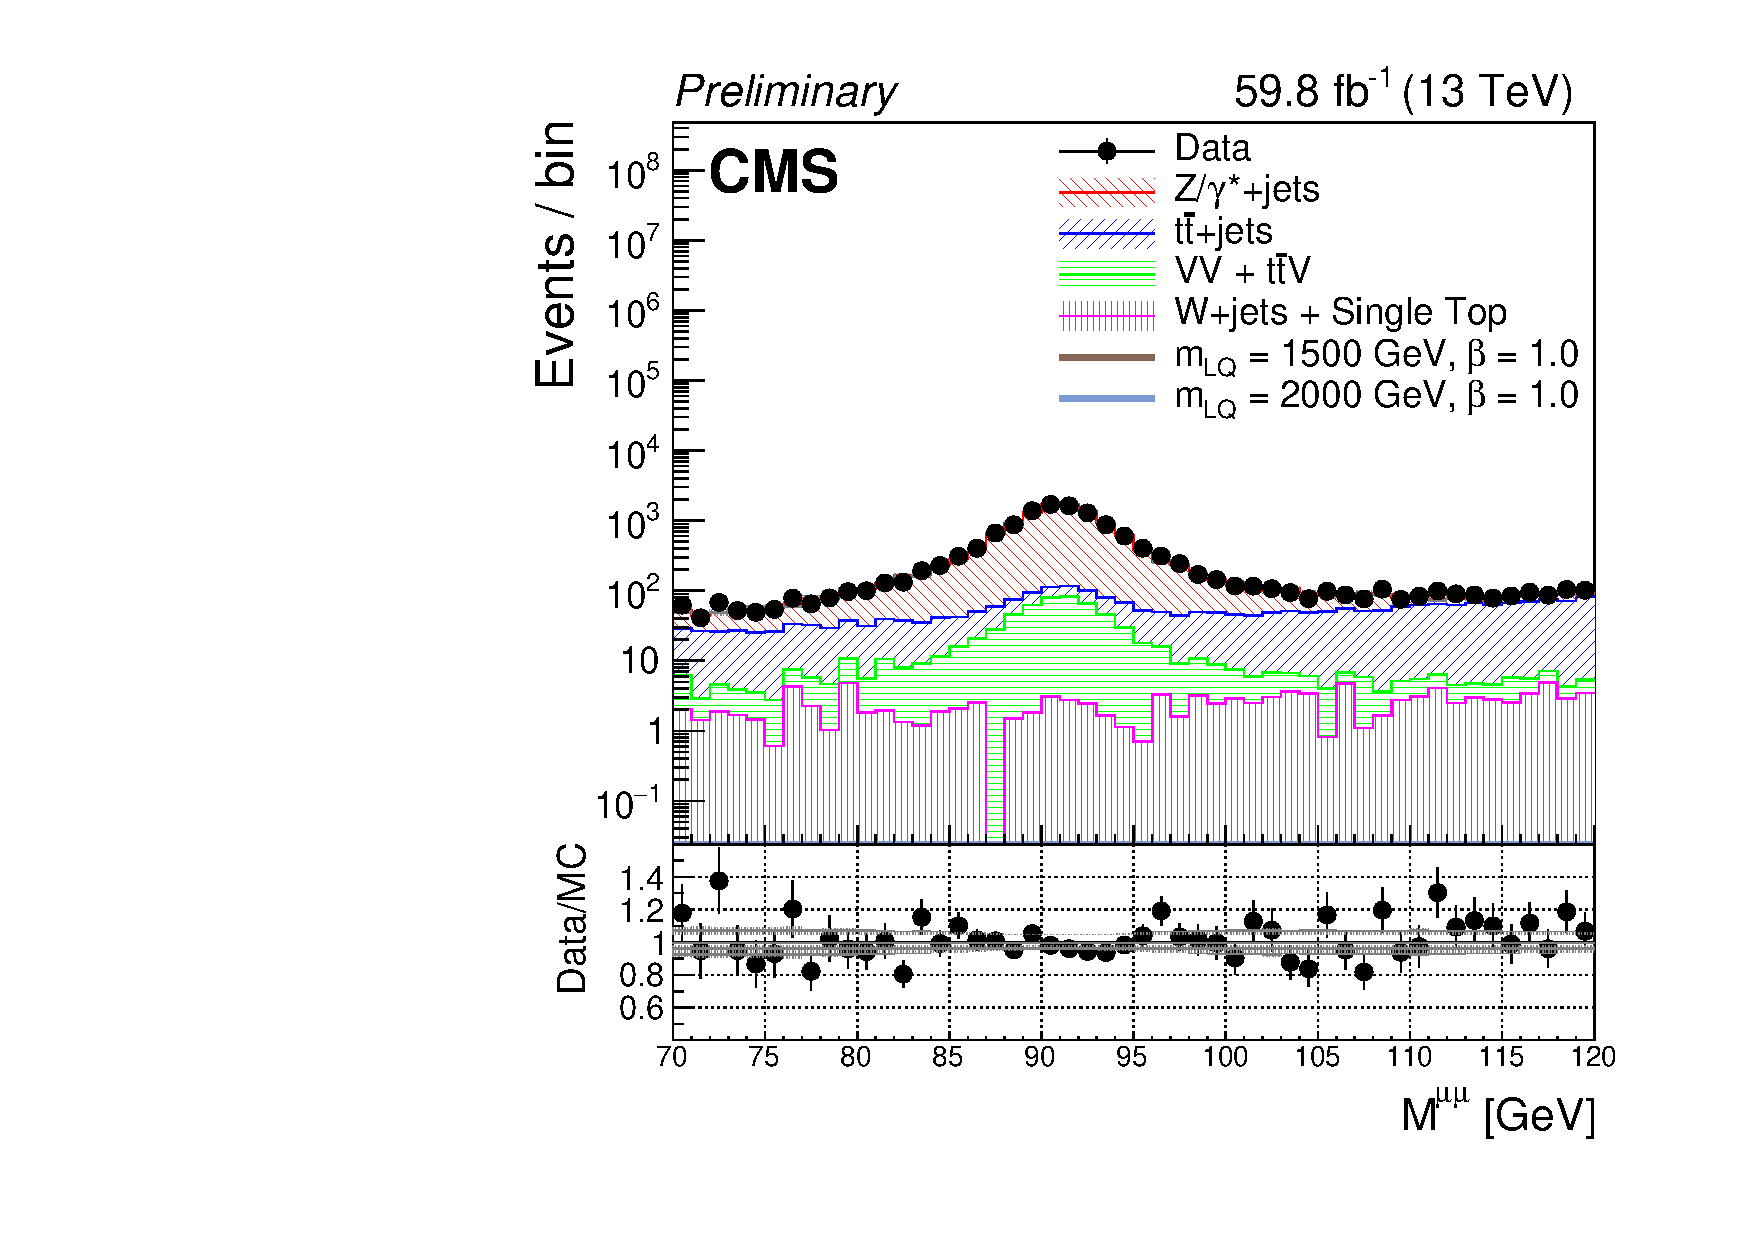
\includegraphics[width=.32\textwidth]{Images/Analysis/Results_2018_Unblinded/Plots/Preselection/BasicLQ_uujj_M_uu_controlzoom_ZRegion.pdf}}
    {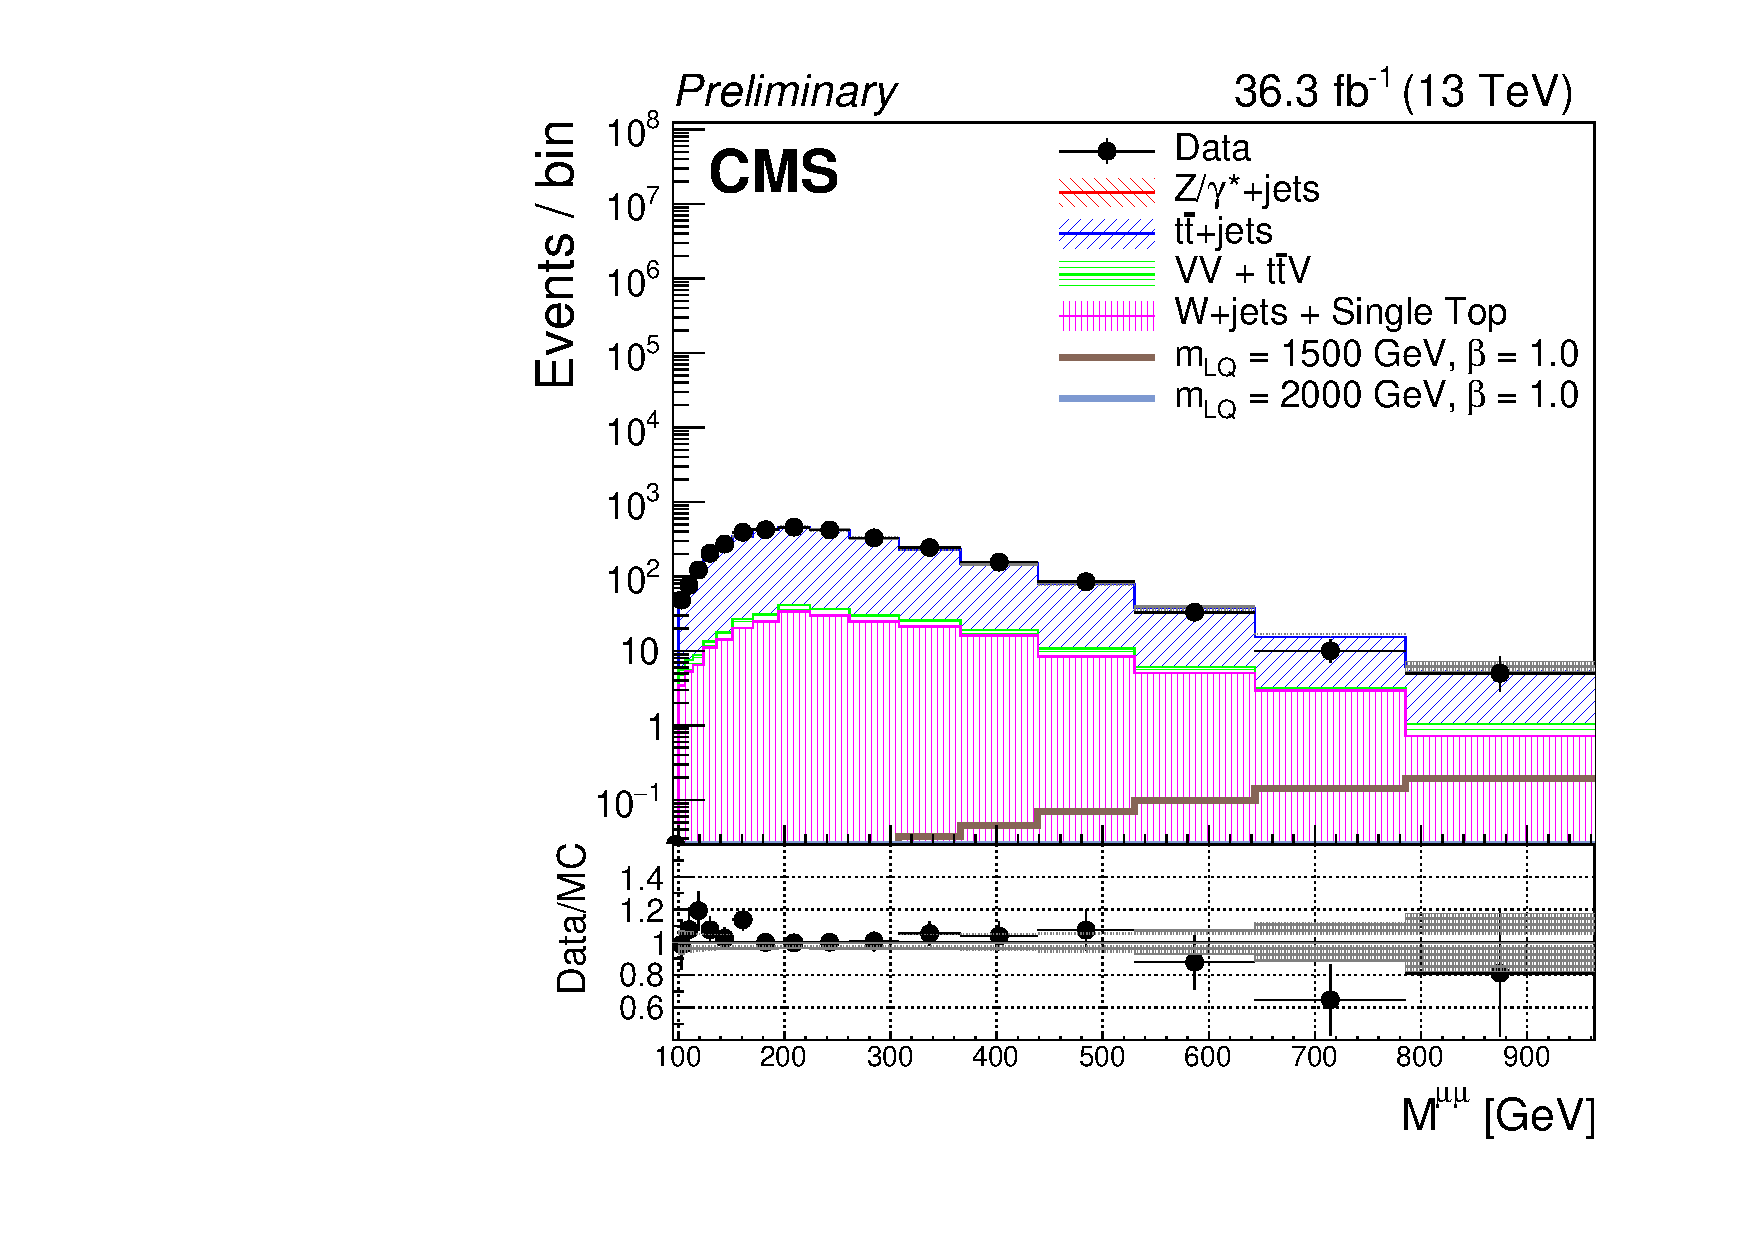
\includegraphics[width=.32\textwidth]{Images/Analysis/Results_2016_Unblinded/Plots/Preselection/BasicLQ_uujj_M_uu_controlzoom_TTRegion.pdf}}
    {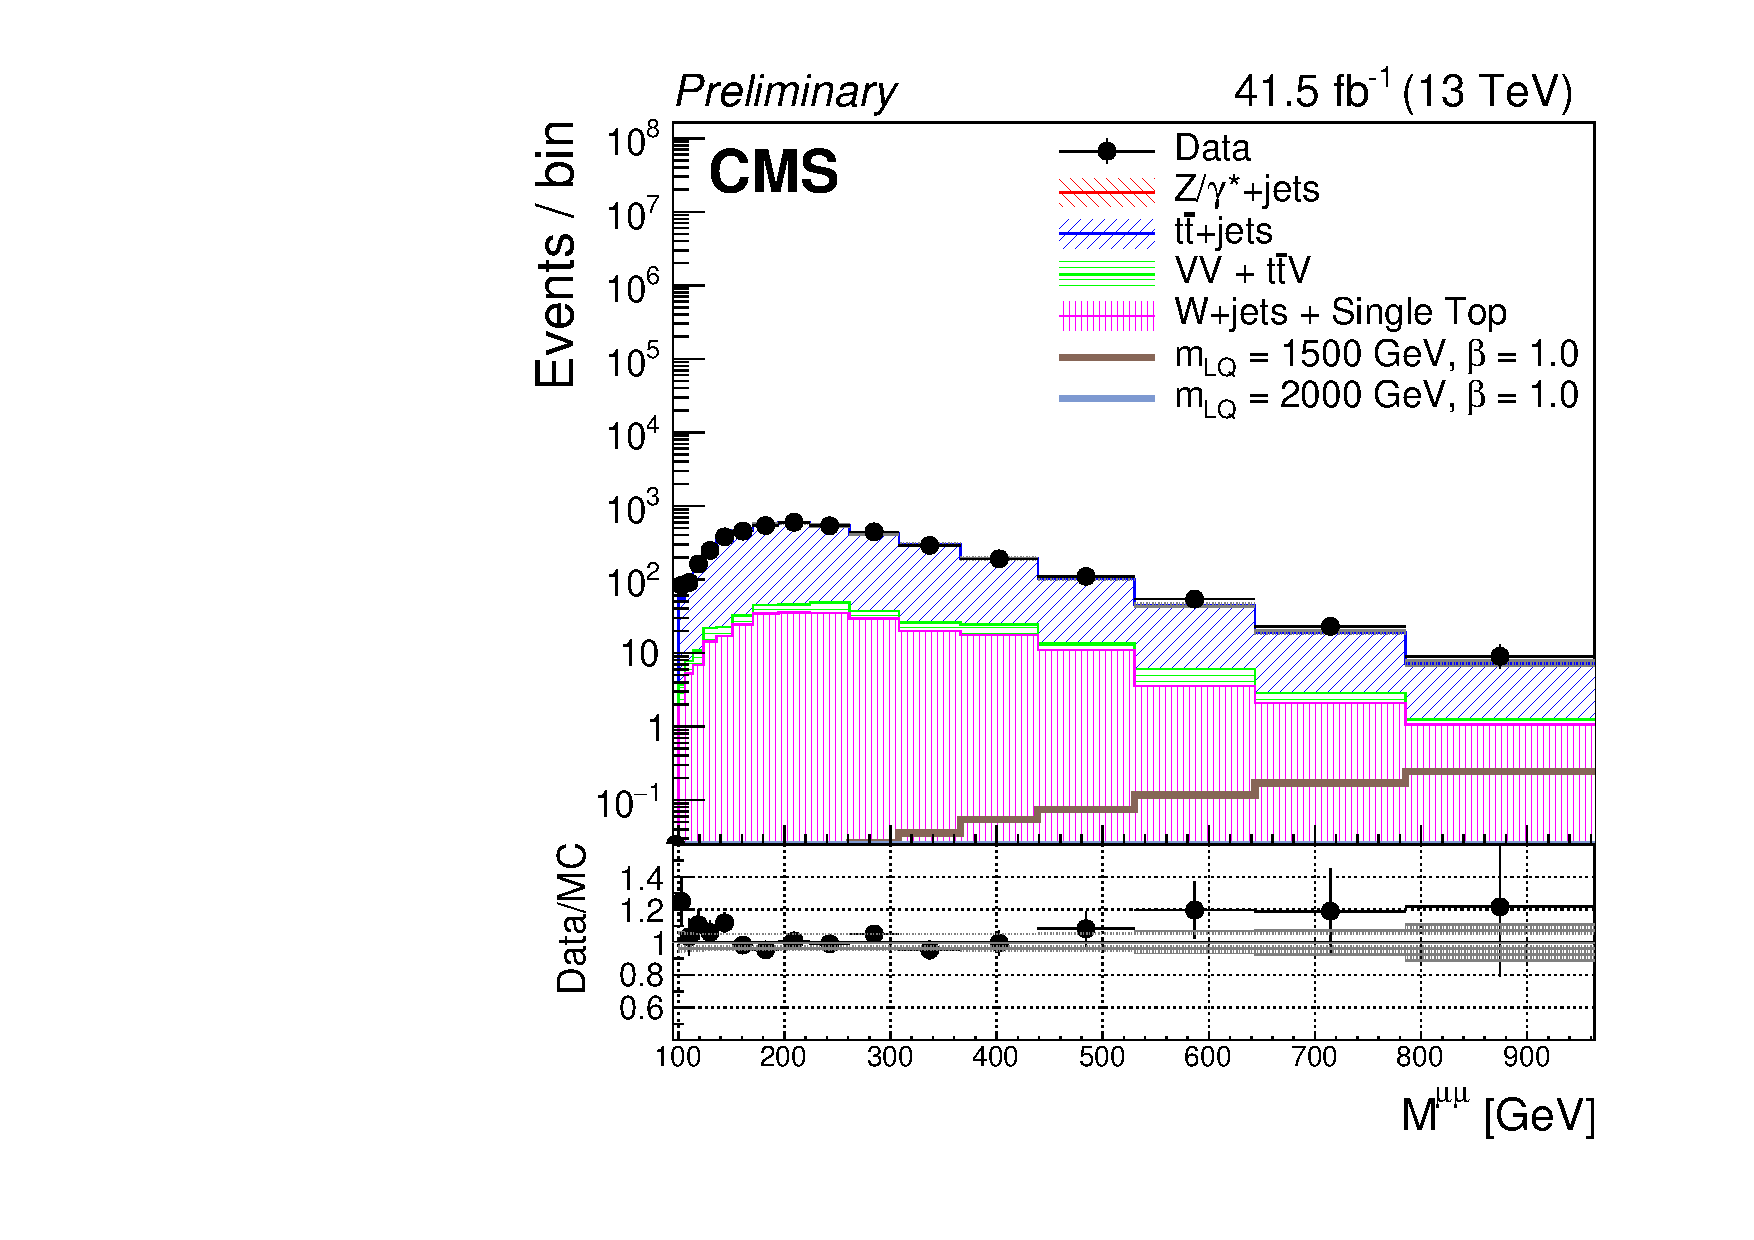
\includegraphics[width=.32\textwidth]{Images/Analysis/Results_2017_Unblinded/Plots/Preselection/BasicLQ_uujj_M_uu_controlzoom_TTRegion.pdf}}
    {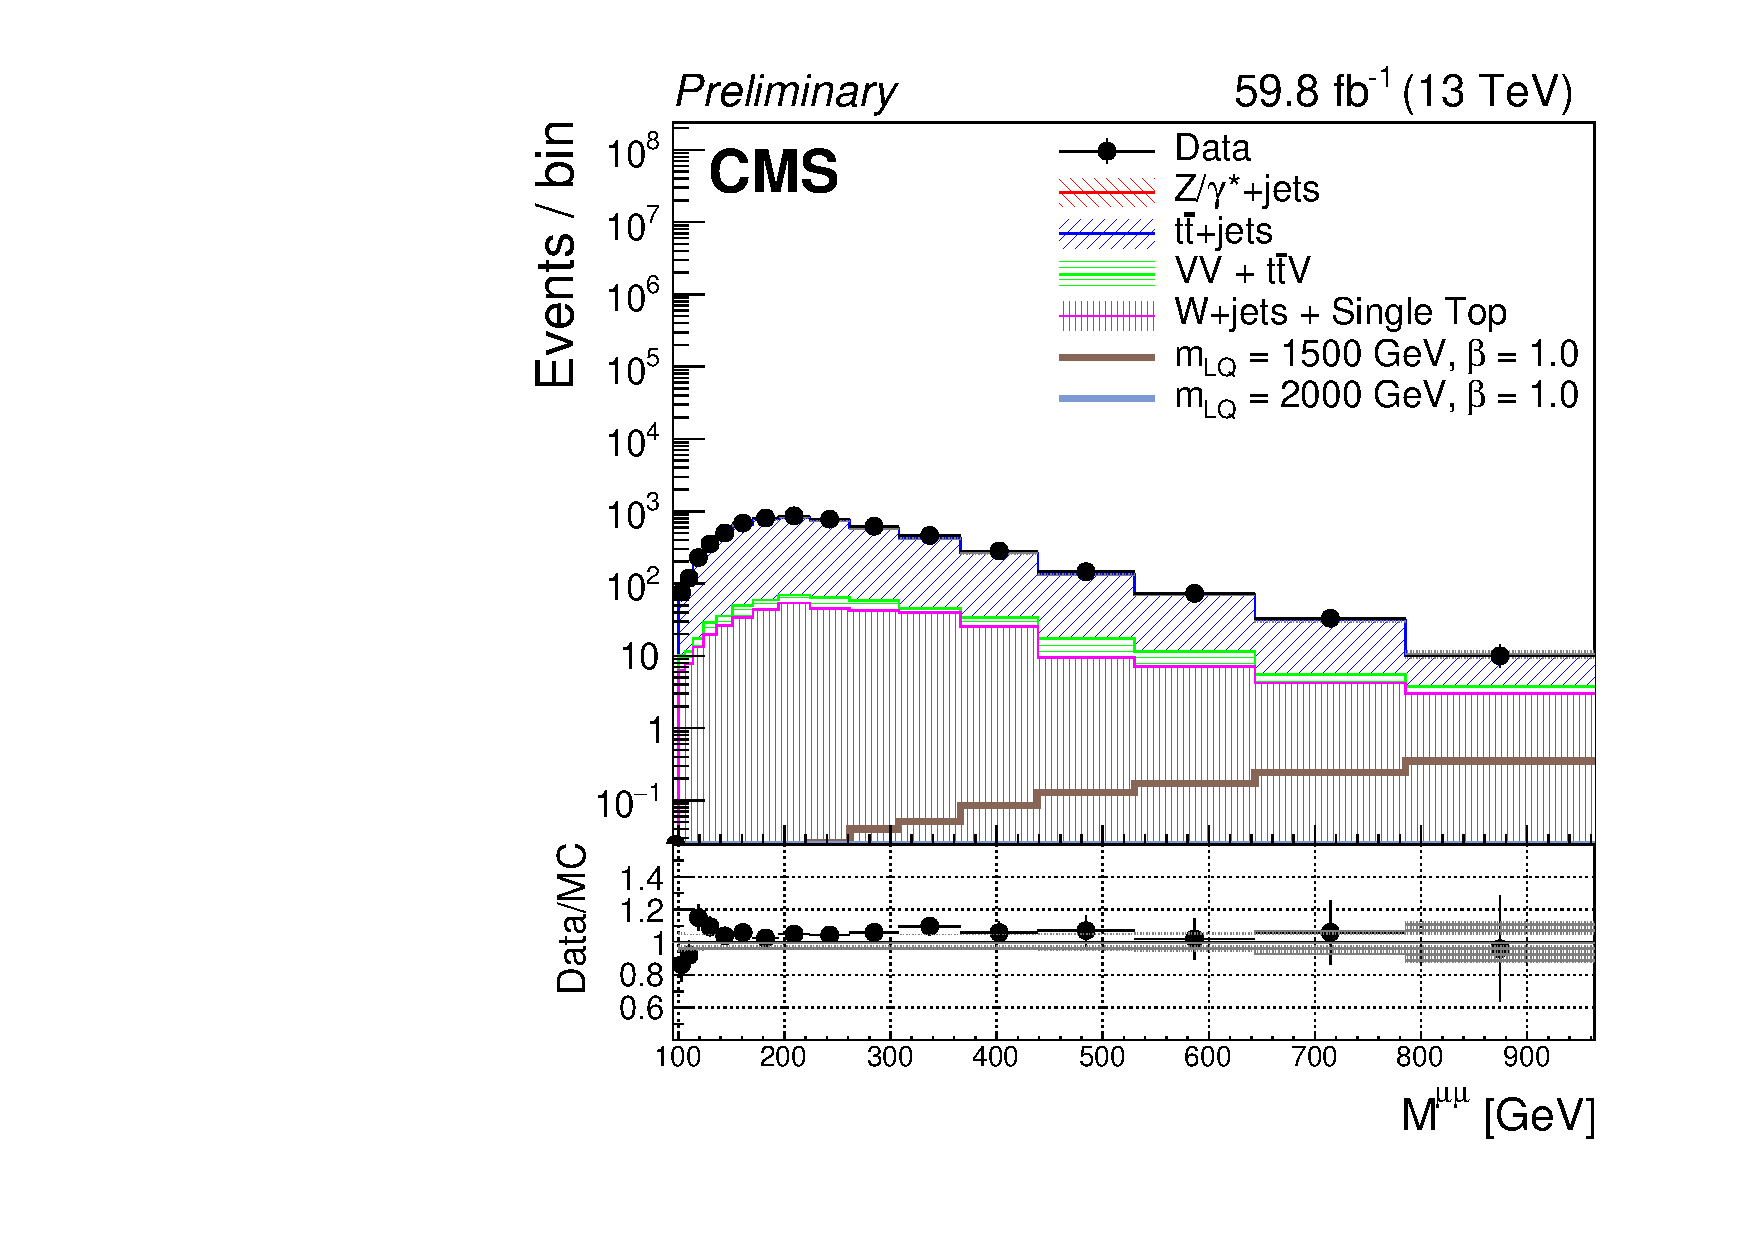
\includegraphics[width=.32\textwidth]{Images/Analysis/Results_2018_Unblinded/Plots/Preselection/BasicLQ_uujj_M_uu_controlzoom_TTRegion.pdf}}
    {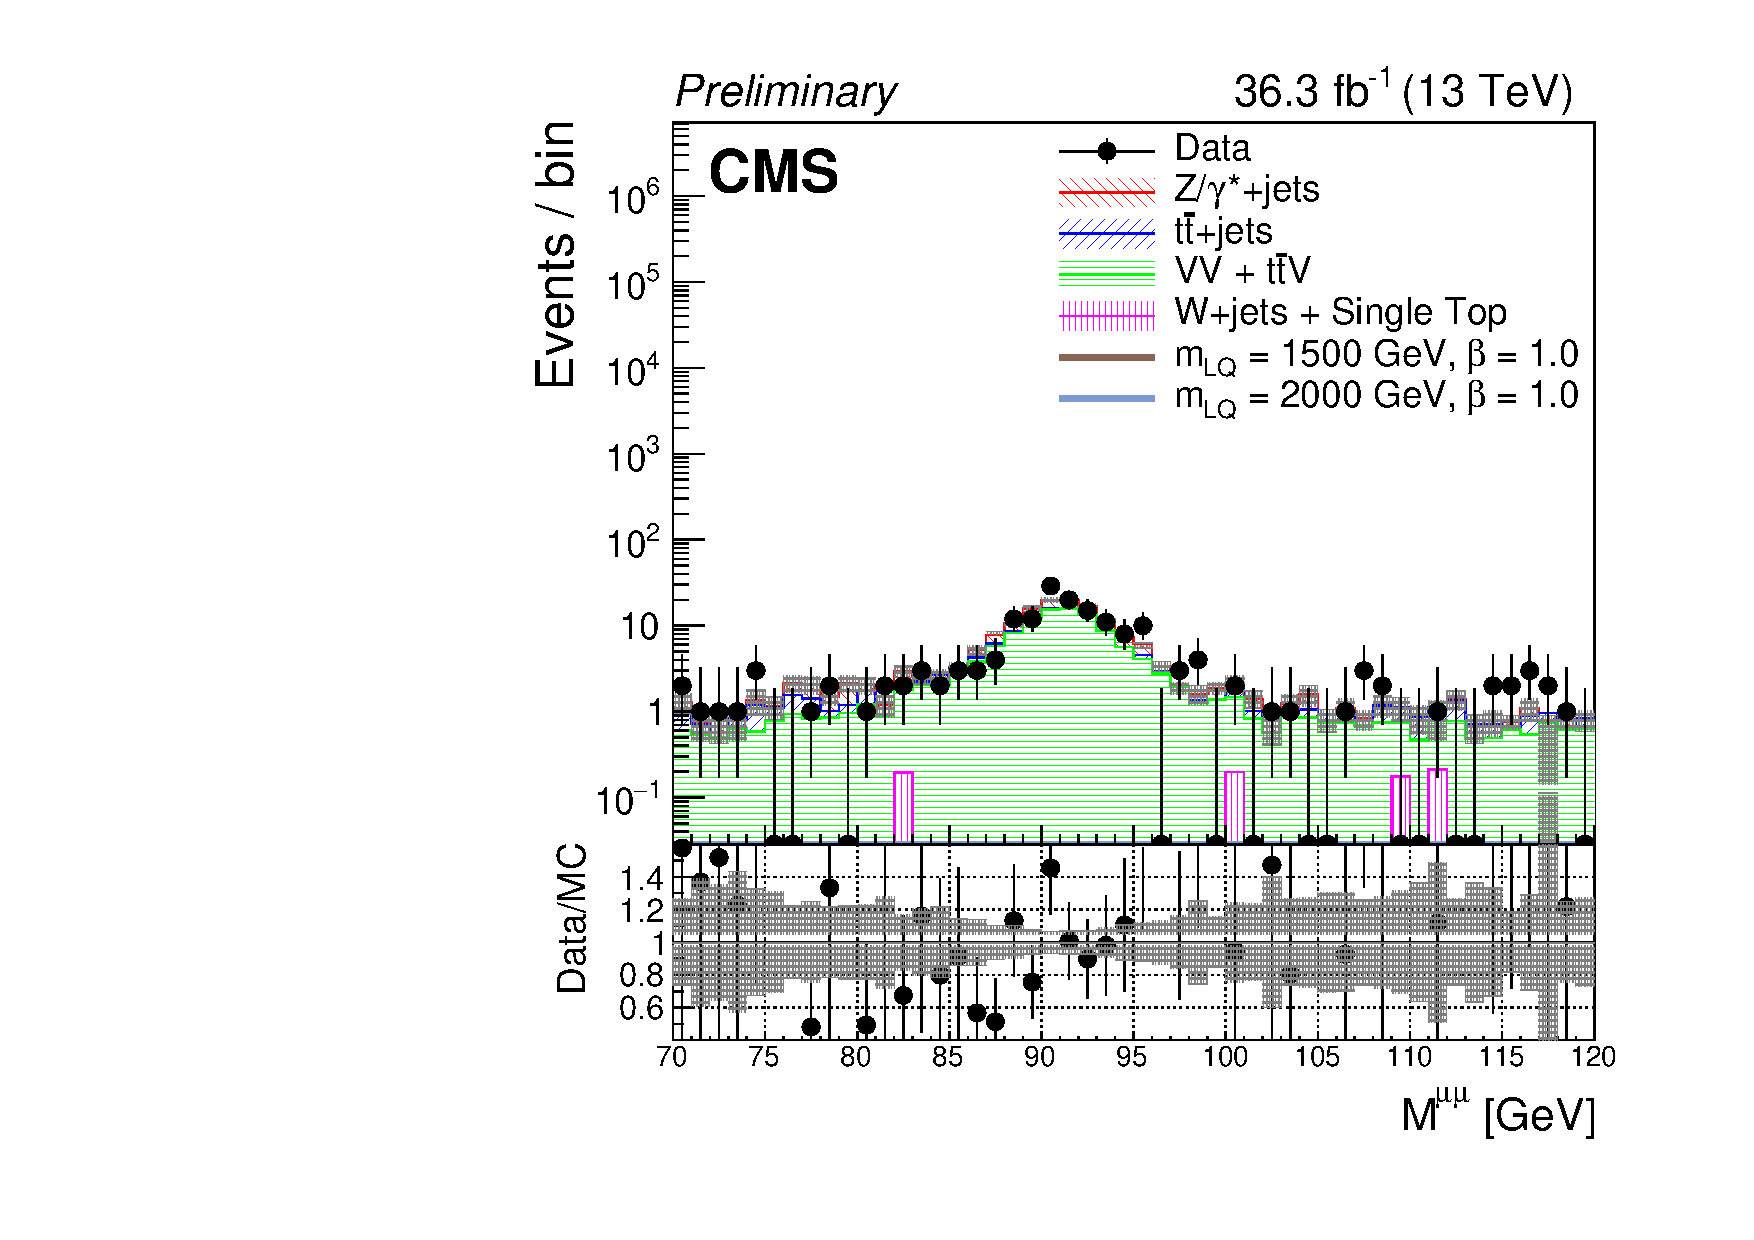
\includegraphics[width=.32\textwidth]{Images/Analysis/Results_2016_Unblinded/Plots/Preselection/BasicLQ_uujj_M_uu_controlzoom_VVRegion.pdf}}
    {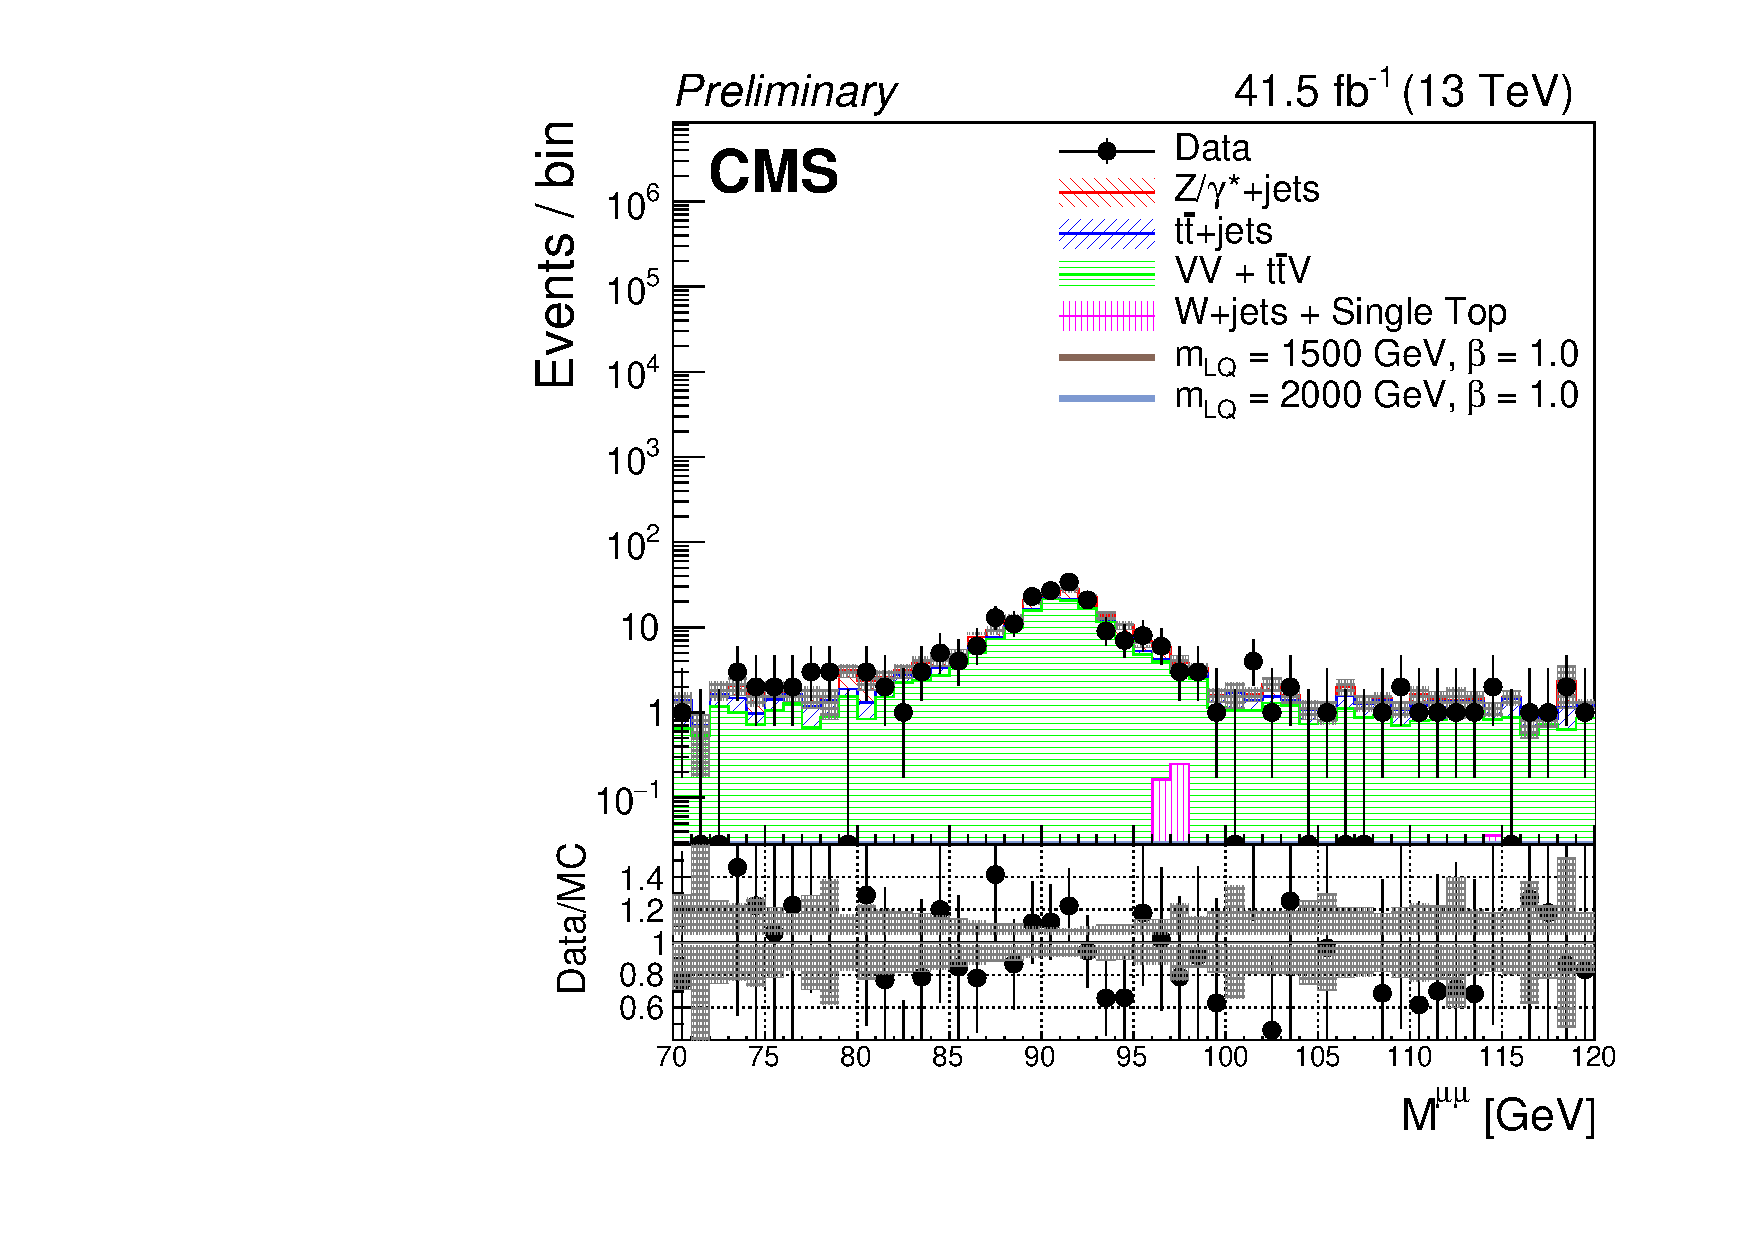
\includegraphics[width=.32\textwidth]{Images/Analysis/Results_2017_Unblinded/Plots/Preselection/BasicLQ_uujj_M_uu_controlzoom_VVRegion.pdf}}
    {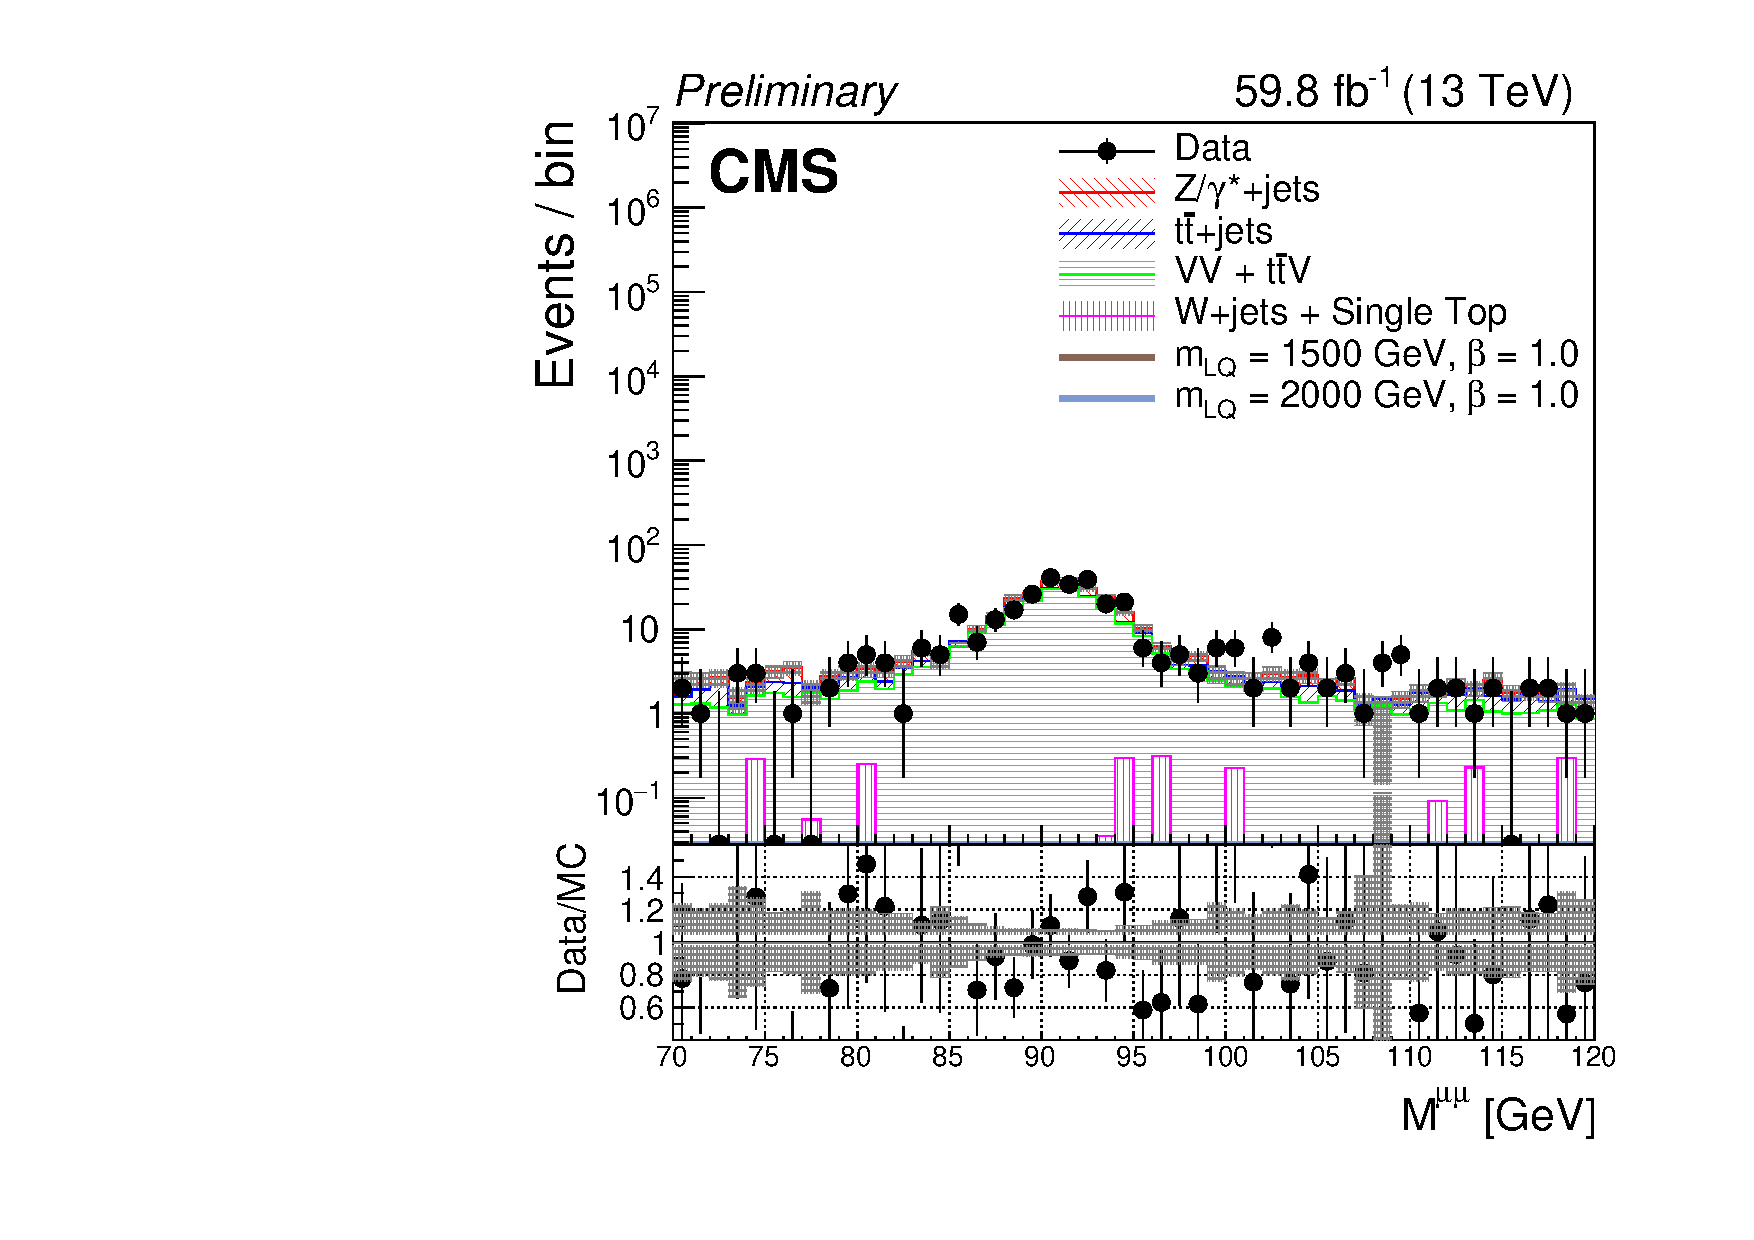
\includegraphics[width=.32\textwidth]{Images/Analysis/Results_2018_Unblinded/Plots/Preselection/BasicLQ_uujj_M_uu_controlzoom_VVRegion.pdf}}
    \caption{A comparison between observed data and SM expectation in \Muu distributions zoomed into the \ZJETS (top), \ttbar (middle), and \VV/\TTV (bottom) CRs at preselection level. Left to right: 2016, 2017, 2018 data. Error bars on observed data points represent statistical uncertainties, and systematic uncertainties on SM expectation are shown by gray hashing.}
    \label{figapp:preselmasszoom}
\end{figure}

\begin{figure}[H]
    \centering
    {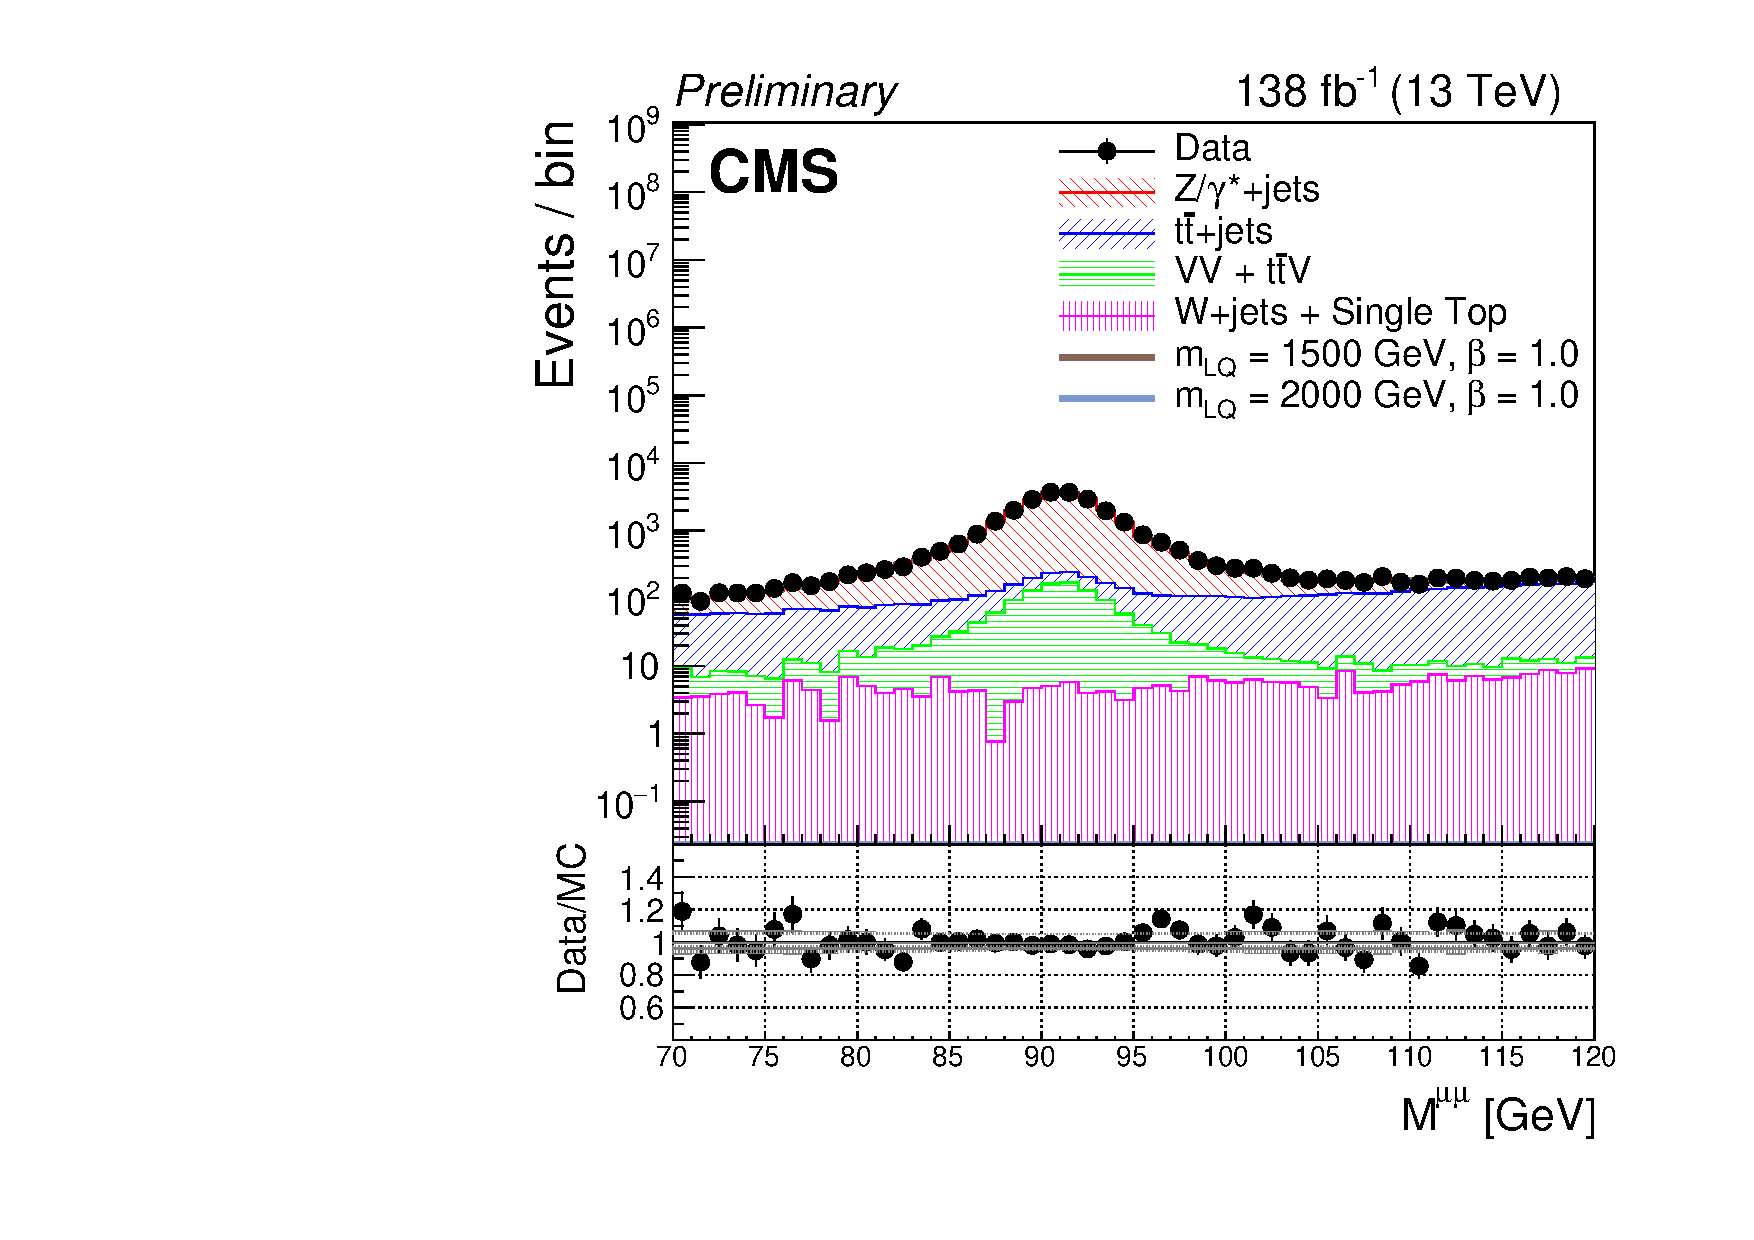
\includegraphics[width=.49\textwidth]{Images/Analysis/Results_combined_Unblinded/Plots/Preselection/BasicLQ_uujj_M_uu_controlzoom_ZRegion.pdf}}
    {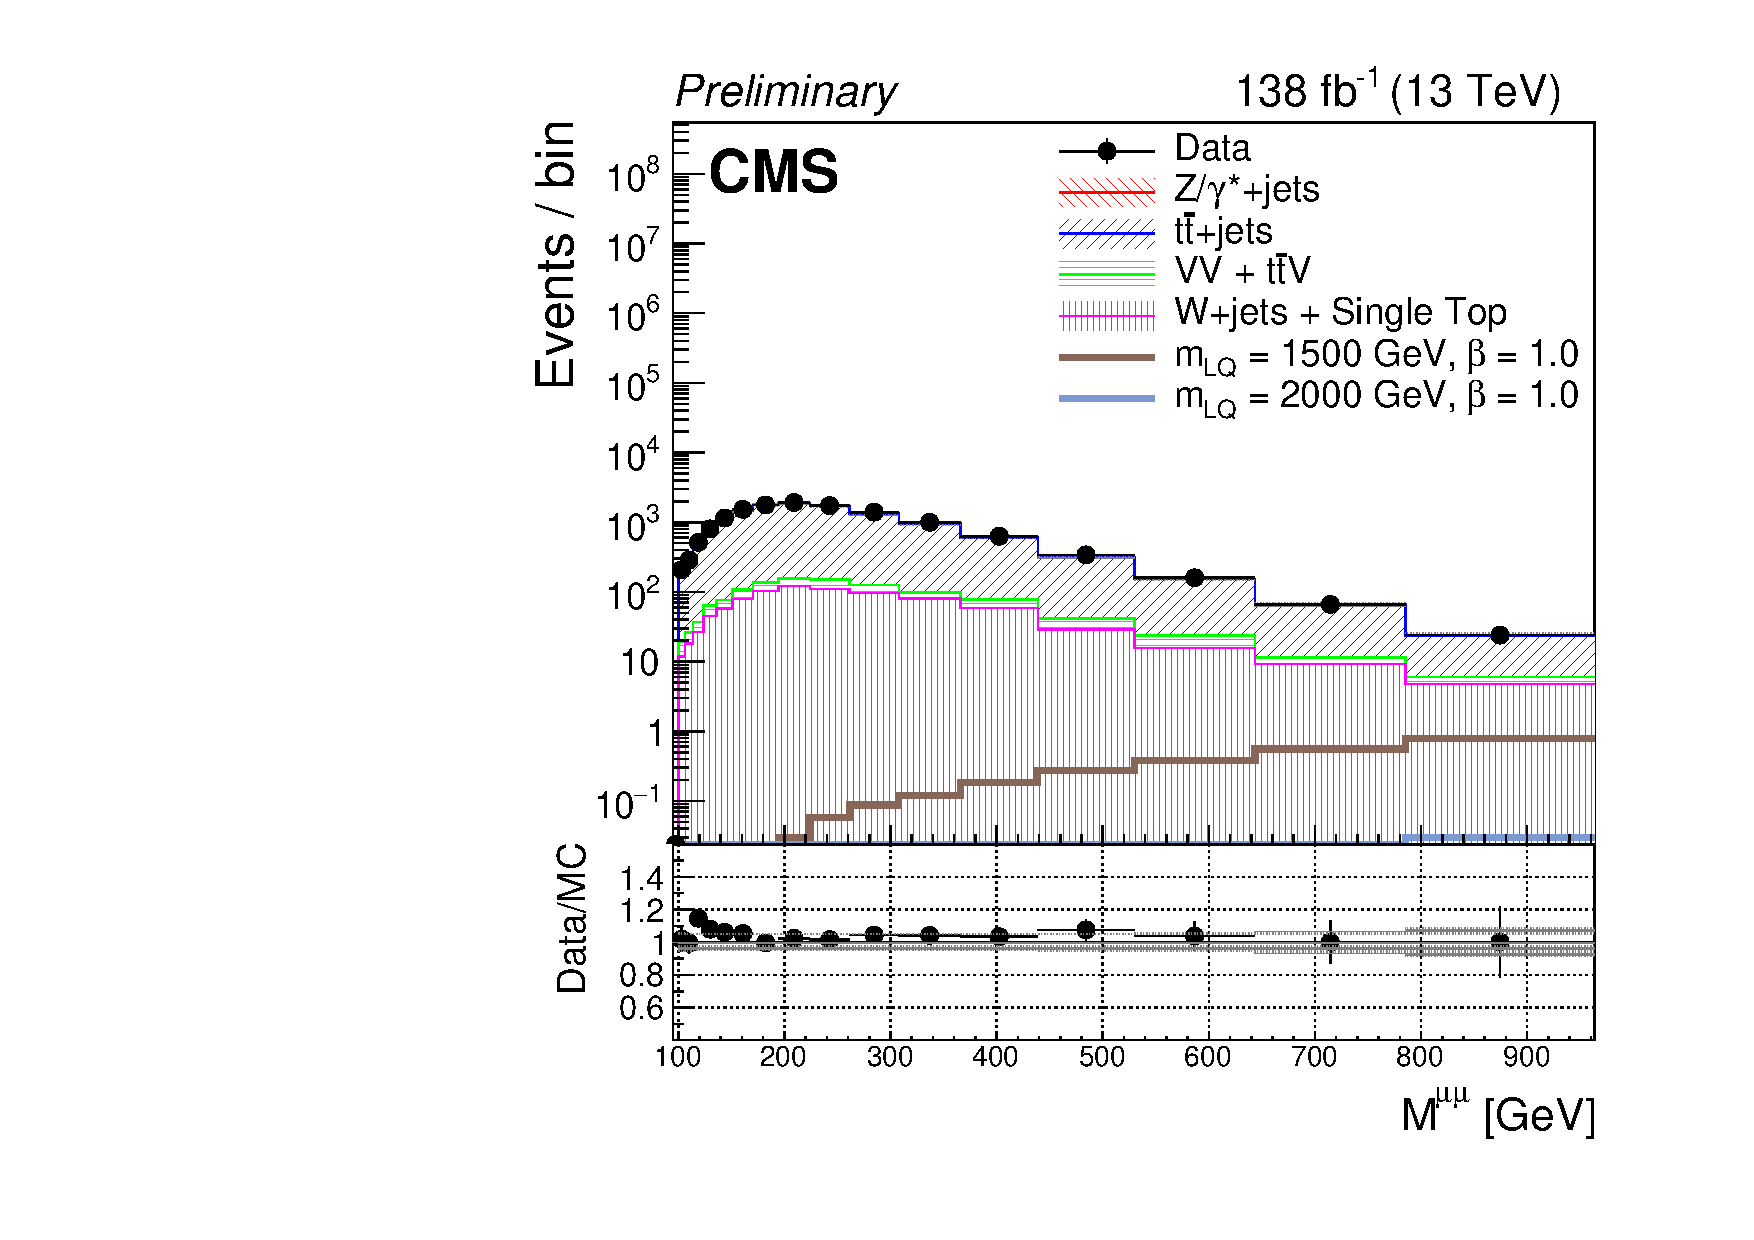
\includegraphics[width=.49\textwidth]{Images/Analysis/Results_combined_Unblinded/Plots/Preselection/BasicLQ_uujj_M_uu_controlzoom_TTRegion.pdf}}
    {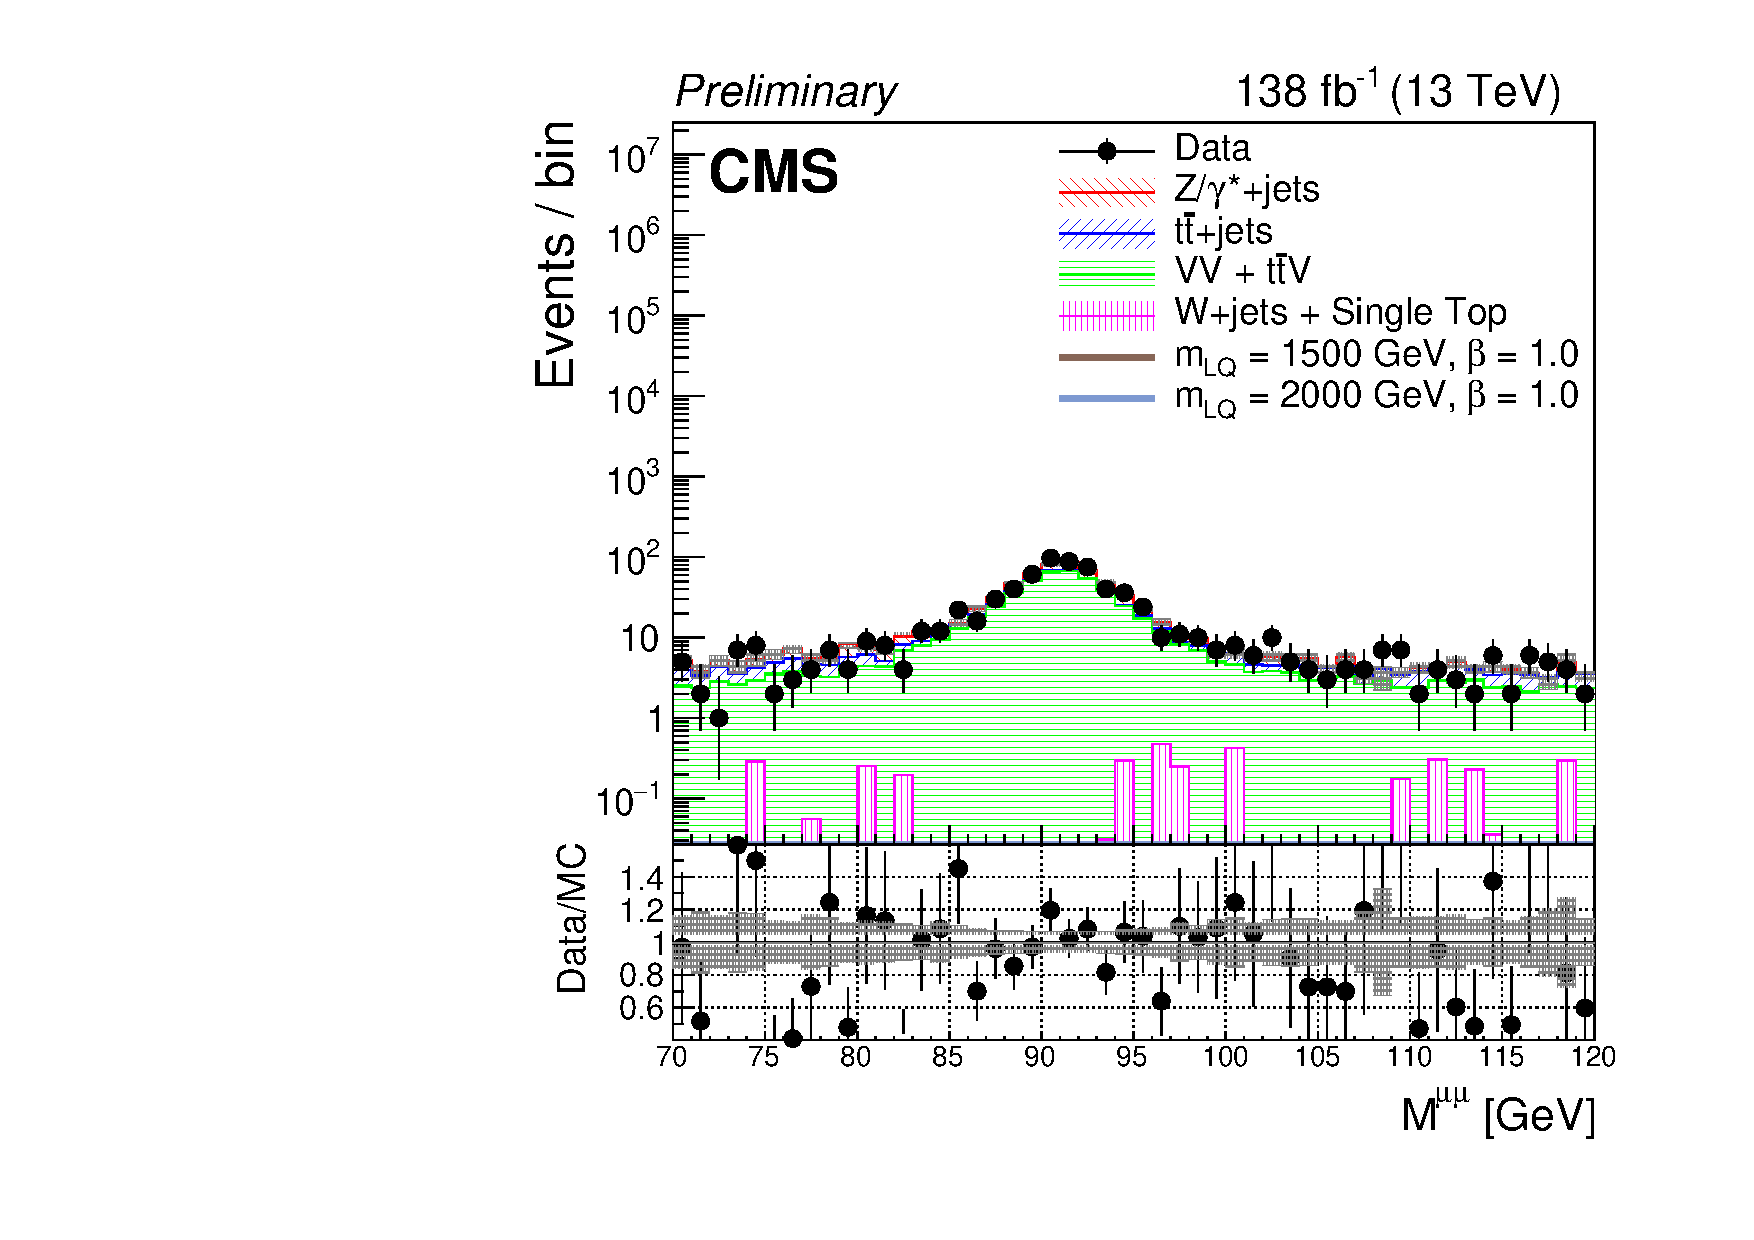
\includegraphics[width=.49\textwidth]{Images/Analysis/Results_combined_Unblinded/Plots/Preselection/BasicLQ_uujj_M_uu_controlzoom_VVRegion.pdf}}
    \caption{A comparison between observed data and SM expectation in \Muu distributions zoomed into the \ZJETS (top-left), \ttbar (top-right), and \VV/\TTV (bottom) CRs at preselection level with the combination of 2016, 2017, and 2018 data. Error bars on observed data points represent statistical uncertainties, and systematic uncertainties on SM expectation are shown by gray hashing.}
    \label{figapp:preselmasszoomcombined}
\end{figure}

\subsection{Data comparison} \label{sec:DataComparison}
Agreement between observed data and SM expectation is found in each year of data-taking, illustrated with the kinematic distributions shown at preselection in Figures~\ref{figapp:vertex}--\ref{figapp:preselbtag}. The combination of data from all three years is provided in Figures~\ref{fig:vertexCombined}--\ref{fig:preselbtagCombined}. In all preselection plots,\ZJETS and \ttbar MC are normalized to data as explained in Section~\ref{sec:BkgNorm}, while the other background MC samples are normalized to the expected number of events (Section~\ref{sec:SimBackground}). Two representative signal MC samples are shown as well ($\MLQ = 1500$ and \SI{2000}{\GeV}), each normalizated to the expected number of events (Section~\ref{sec:SimSignal}). All events must satisfy the b-jet tag requirement from Section~\ref{sec:BJetTagging}, and signal and background events have been corrected according to Section~\ref{sec:Corrections}. The kinematic distributions plotted, most of which are inputs to the final selection, include the momenta and spatial separation of final state objects, invariant masses, MET, object multiplicities, and DeepJet b tag scores. Additionally, we define a few variables that are either arcane or unique to this analysis. The kinematic \ST is the scalar sum of the \pt of the four final state objects:

\begin{equation}
       \ST = \pt(\PmuOne) + \pt(\PmuTwo) + \pt(\PjOne) + \pt(\PjTwo).
\end{equation}

The leptoquark candidates, identified as muon-jet invariant masses \MujOne and \MujTwo, are defined as the muon-jet pairings that minimize the absolute difference between the two masses, with \MujOne being the larger mass:

\begin{equation}
       \mathrm{min}\left( | \MujOne - \MujTwo | \right), \MujOne > \MujTwo
\end{equation}

The kinematics we have defined---\ST, \MujOne and \MujTwo---are particularly strong signal/background discriminators, making them indespensible variables to the final selection, as explained in Section~\ref{sec:FinalSelection}.

\begin{figure}[H]
       \centering
       {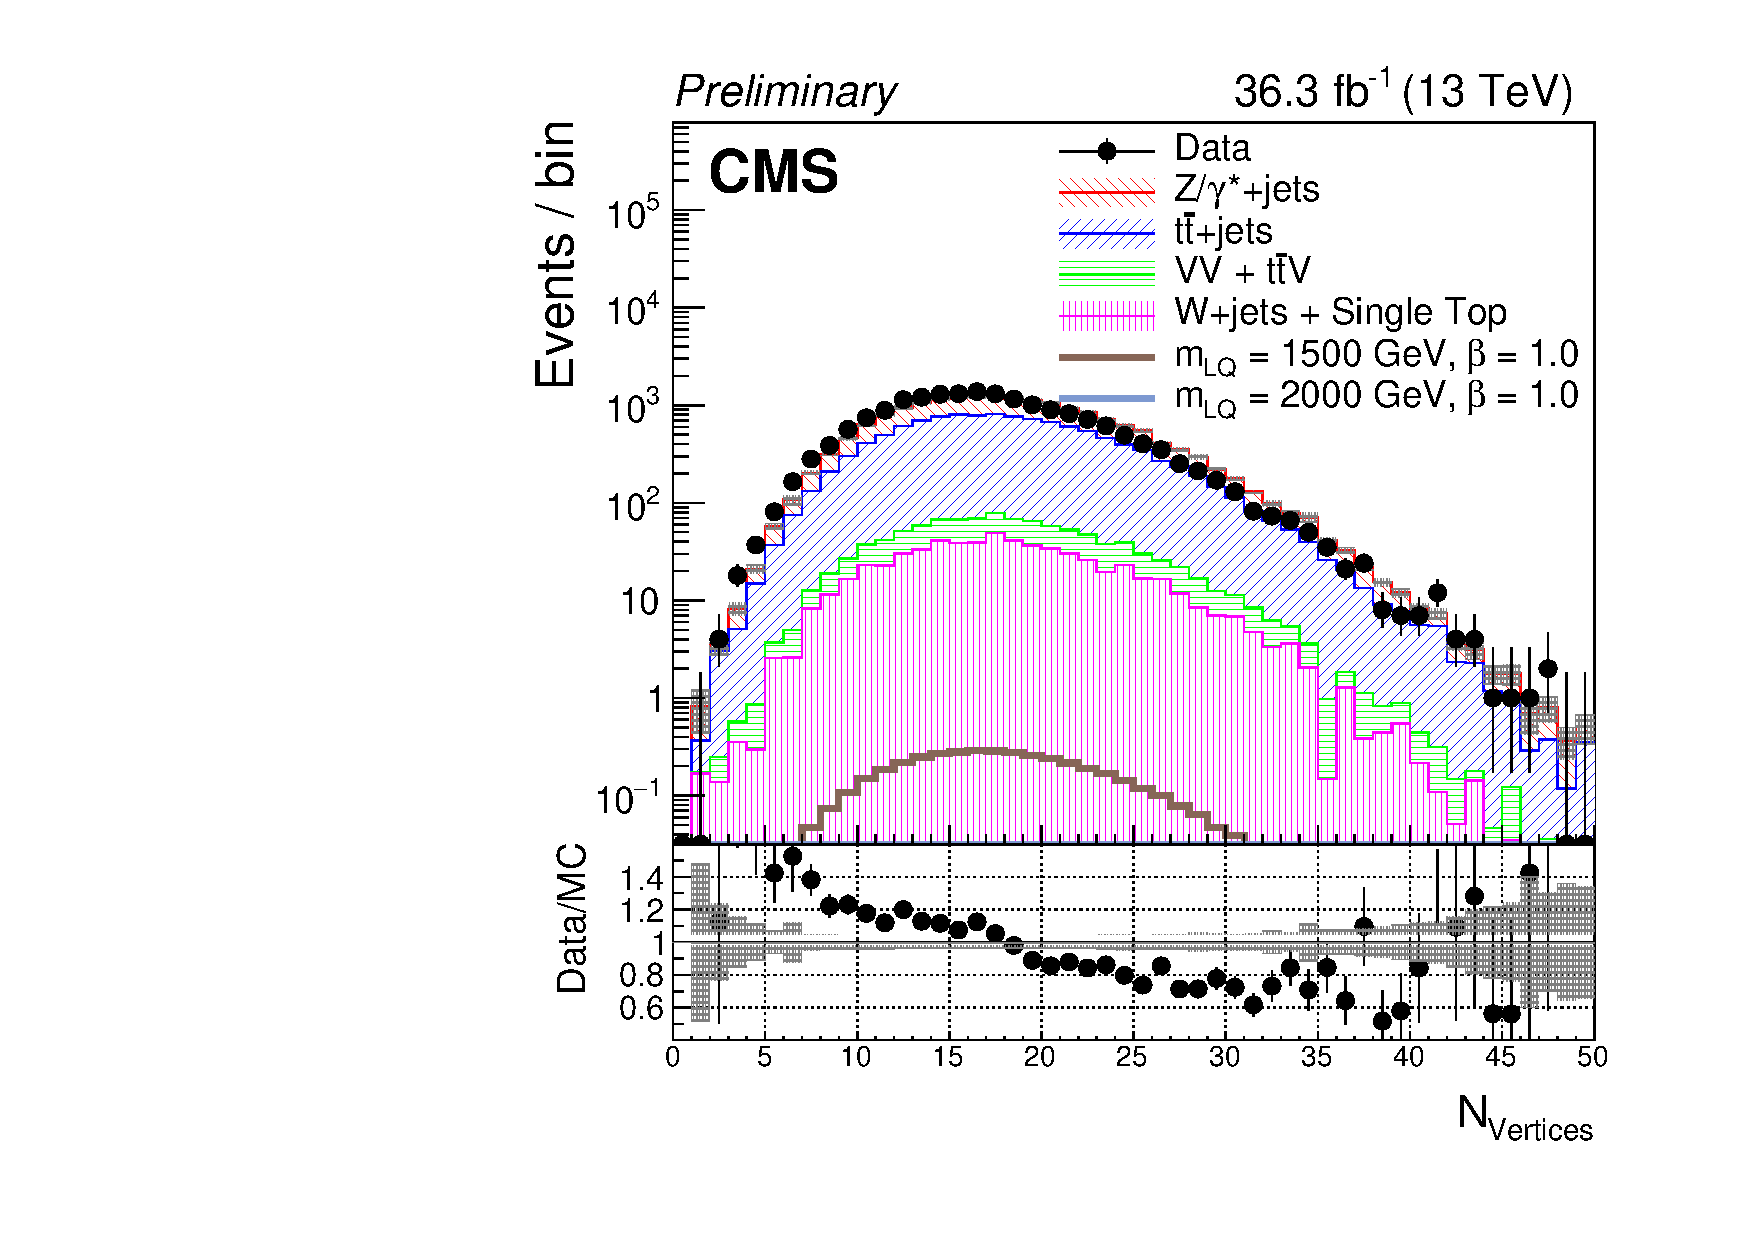
\includegraphics[width=.32\textwidth]{Images/Analysis/Results_2016_Unblinded/Plots/Preselection/BasicLQ_uujj_GoodVertexCount_standard.pdf}}
       {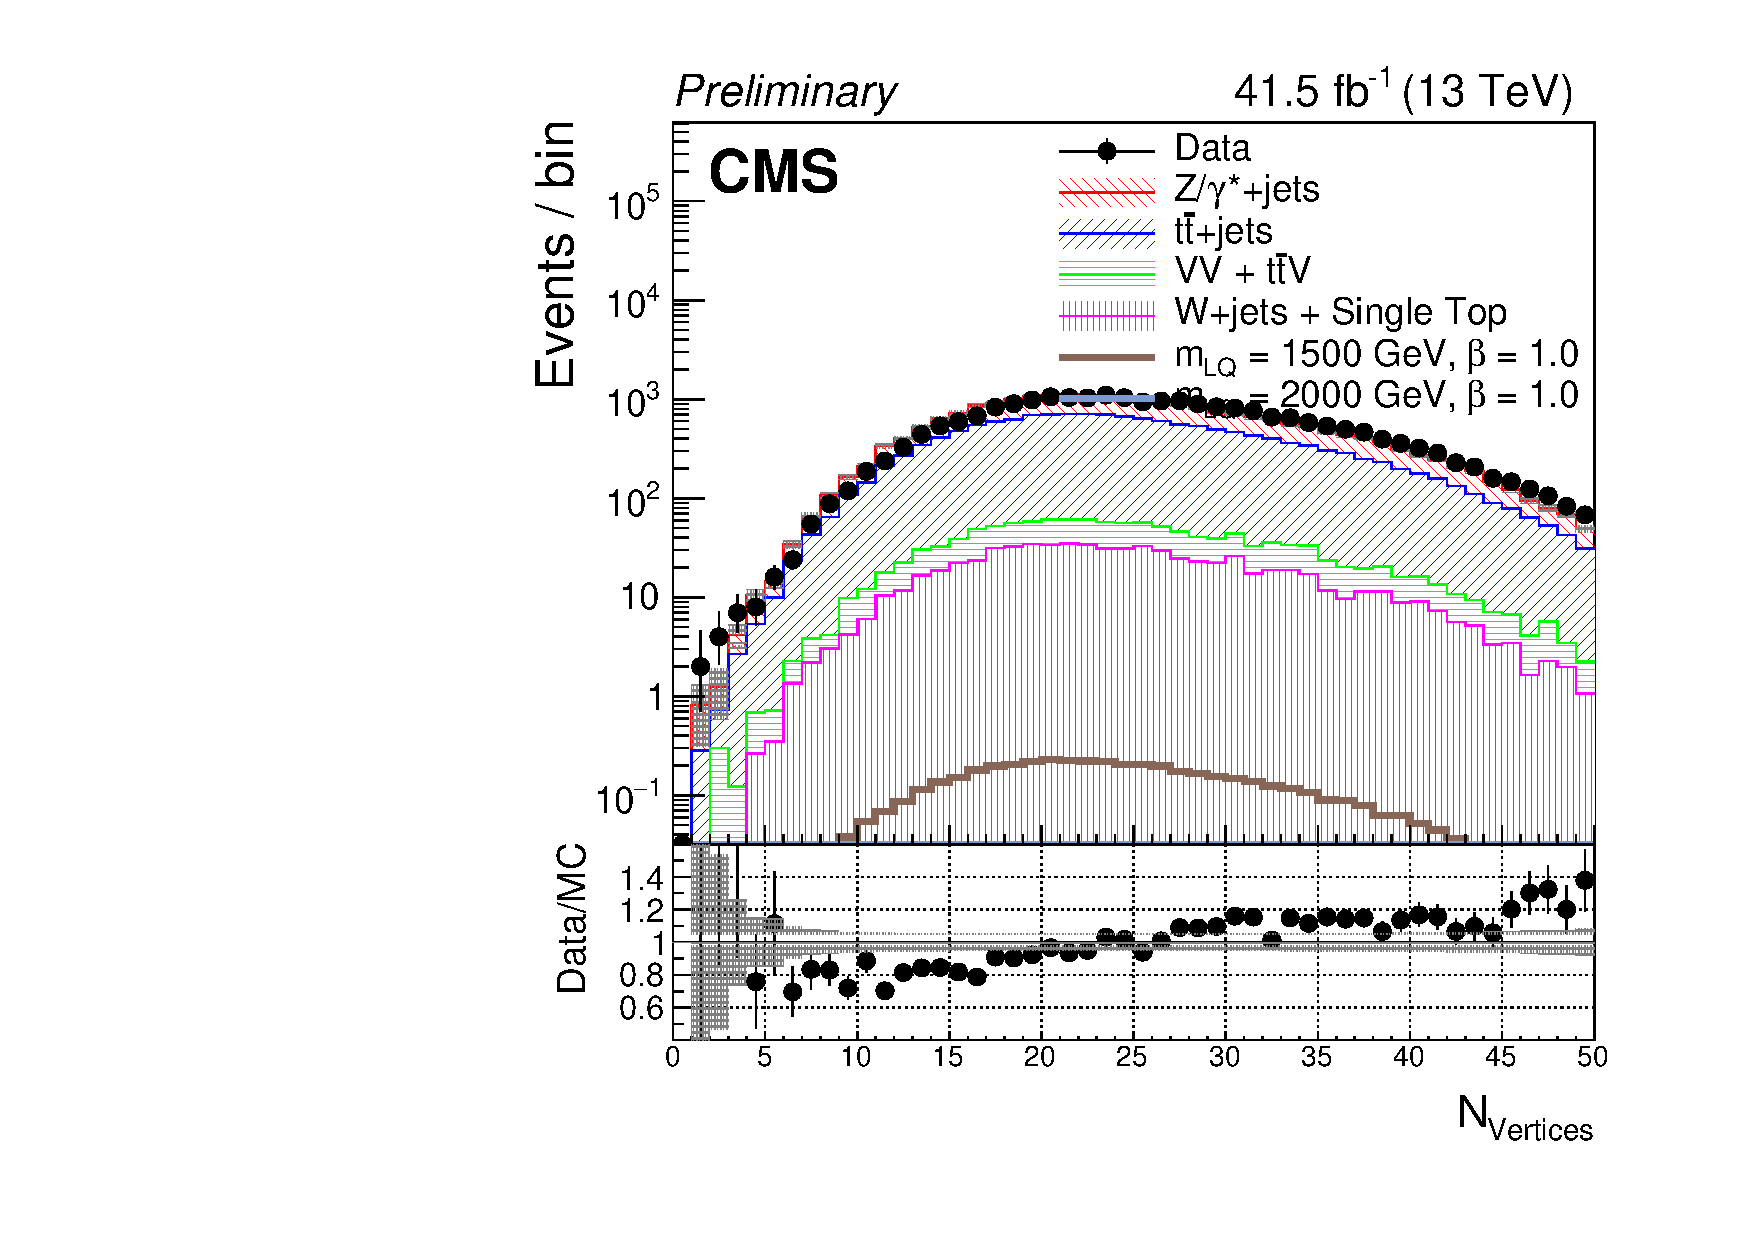
\includegraphics[width=.32\textwidth]{Images/Analysis/Results_2017_Unblinded/Plots/Preselection/BasicLQ_uujj_GoodVertexCount_standard.pdf}}
       {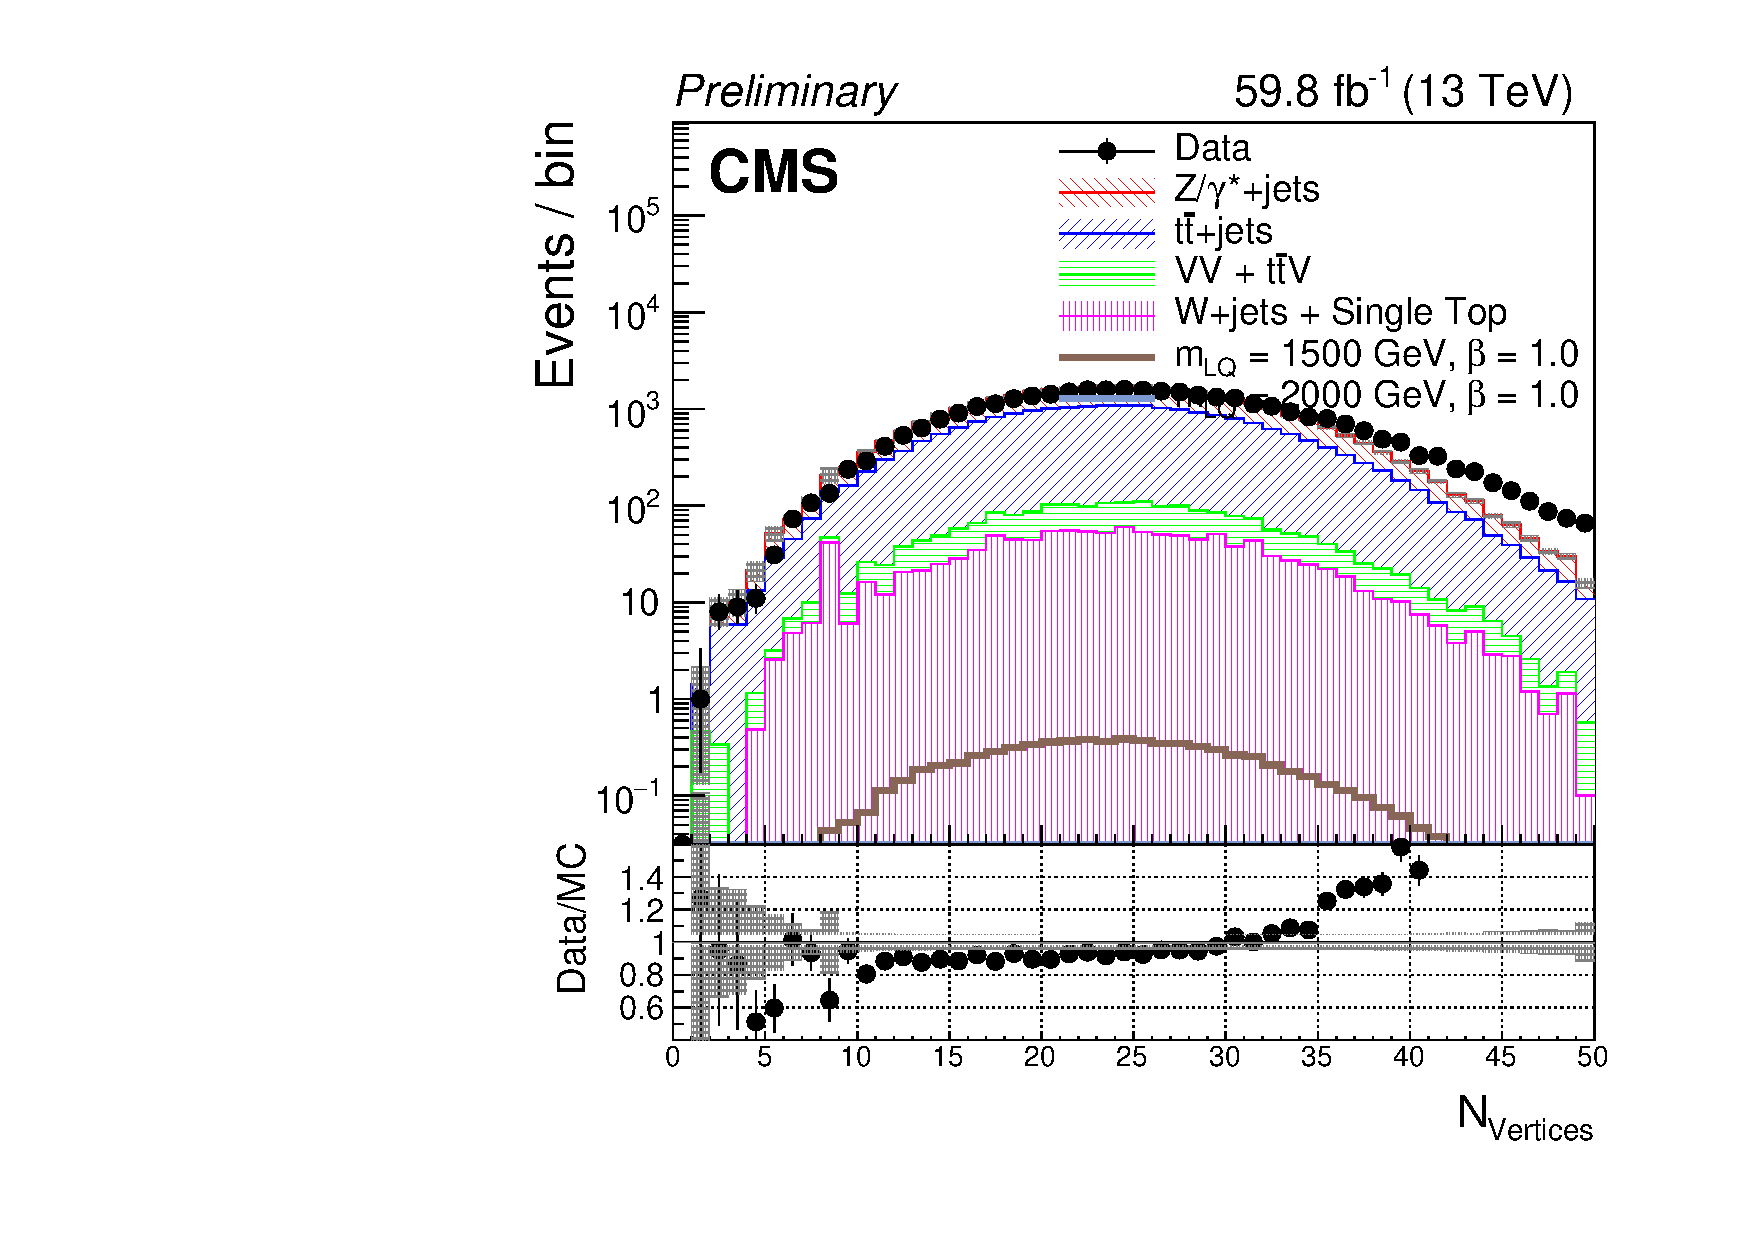
\includegraphics[width=.32\textwidth]{Images/Analysis/Results_2018_Unblinded/Plots/Preselection/BasicLQ_uujj_GoodVertexCount_standard.pdf}}
       \caption{A comparison of the number of reconstructed vertices at preselection level in 2016 (left), 2017 (middle) and 2018 (right) data. Error bars shown represent statistical uncertainties, and systematic uncertainties are shown by gray hashing.}
       \label{figapp:vertex}
\end{figure}
\begin{figure}[H]
       \centering
       {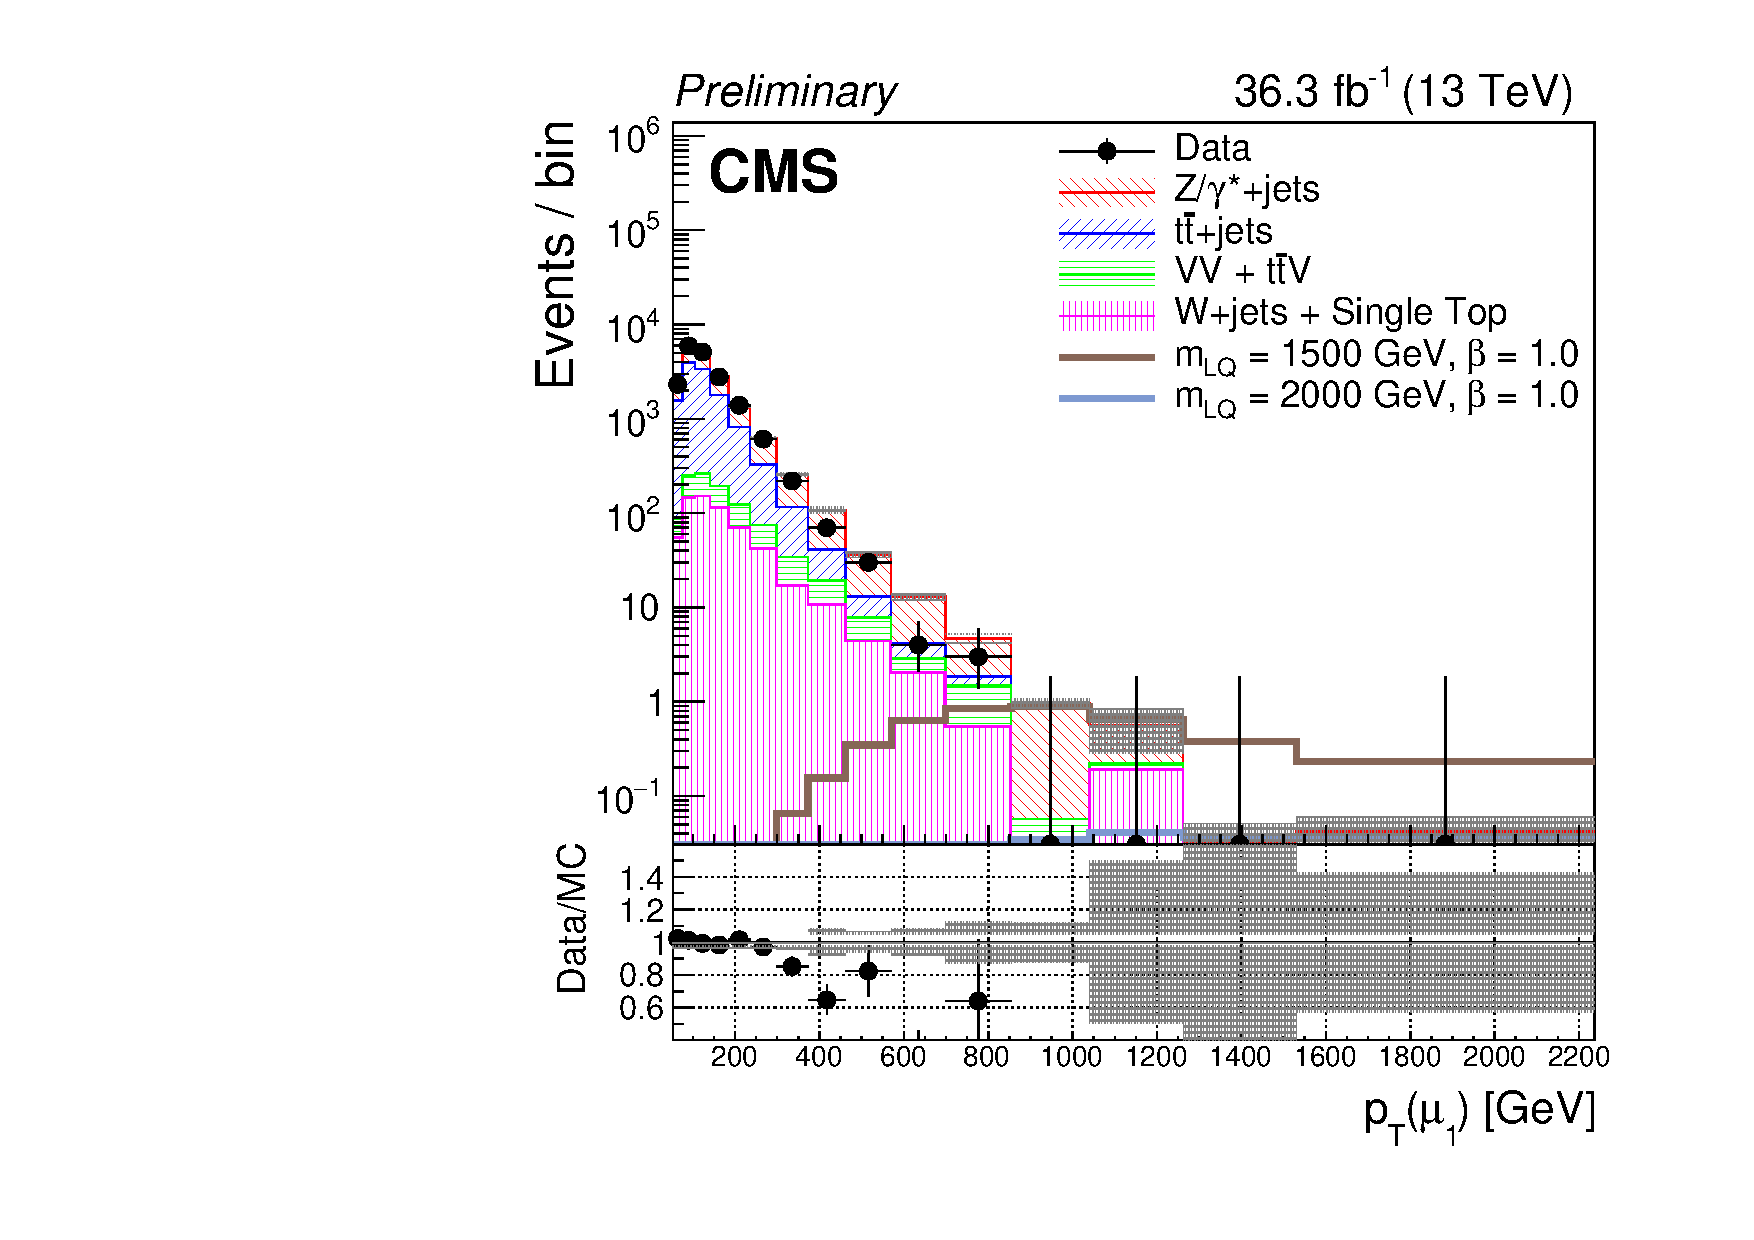
\includegraphics[width=.32\textwidth]{Images/Analysis/Results_2016_Unblinded/Plots/Preselection/BasicLQ_uujj_Pt_muon1_standard.pdf}}
       {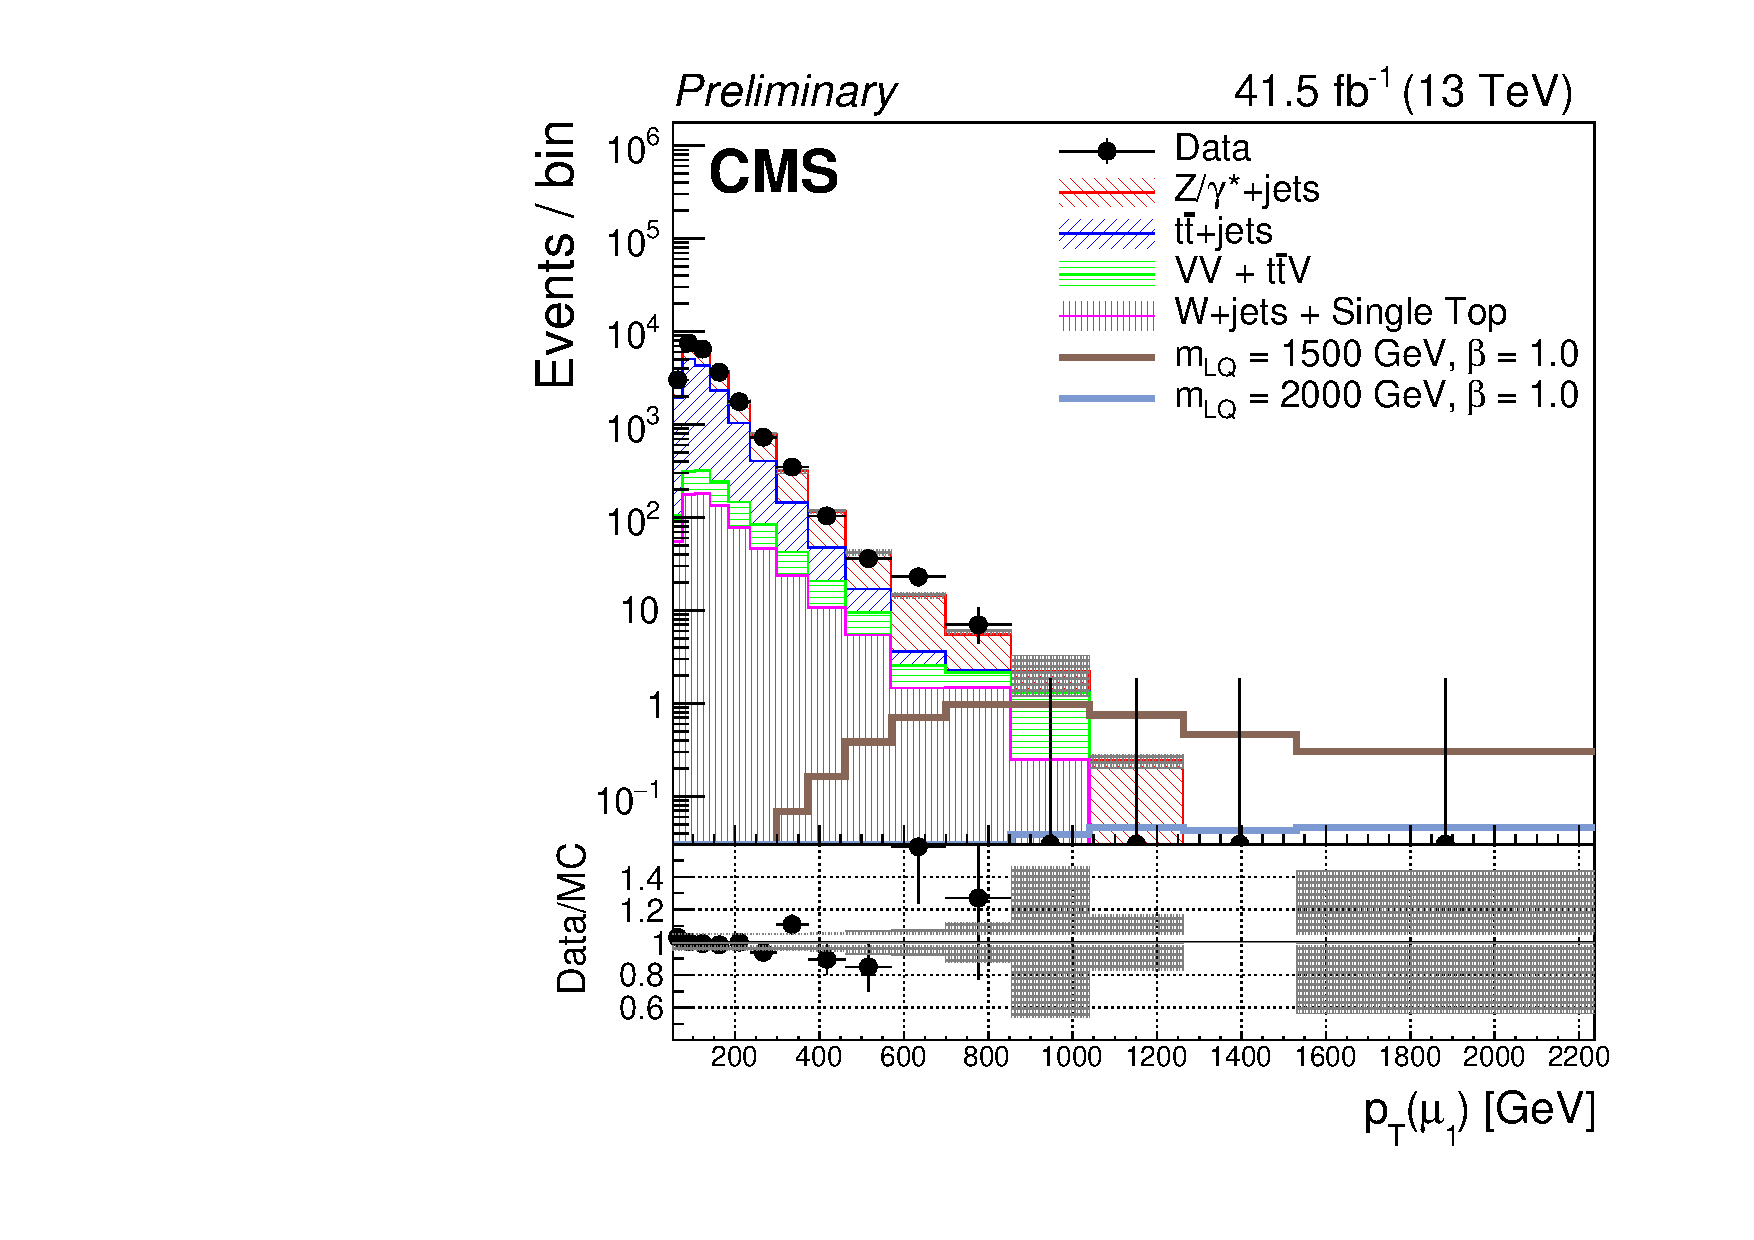
\includegraphics[width=.32\textwidth]{Images/Analysis/Results_2017_Unblinded/Plots/Preselection/BasicLQ_uujj_Pt_muon1_standard.pdf}}
       {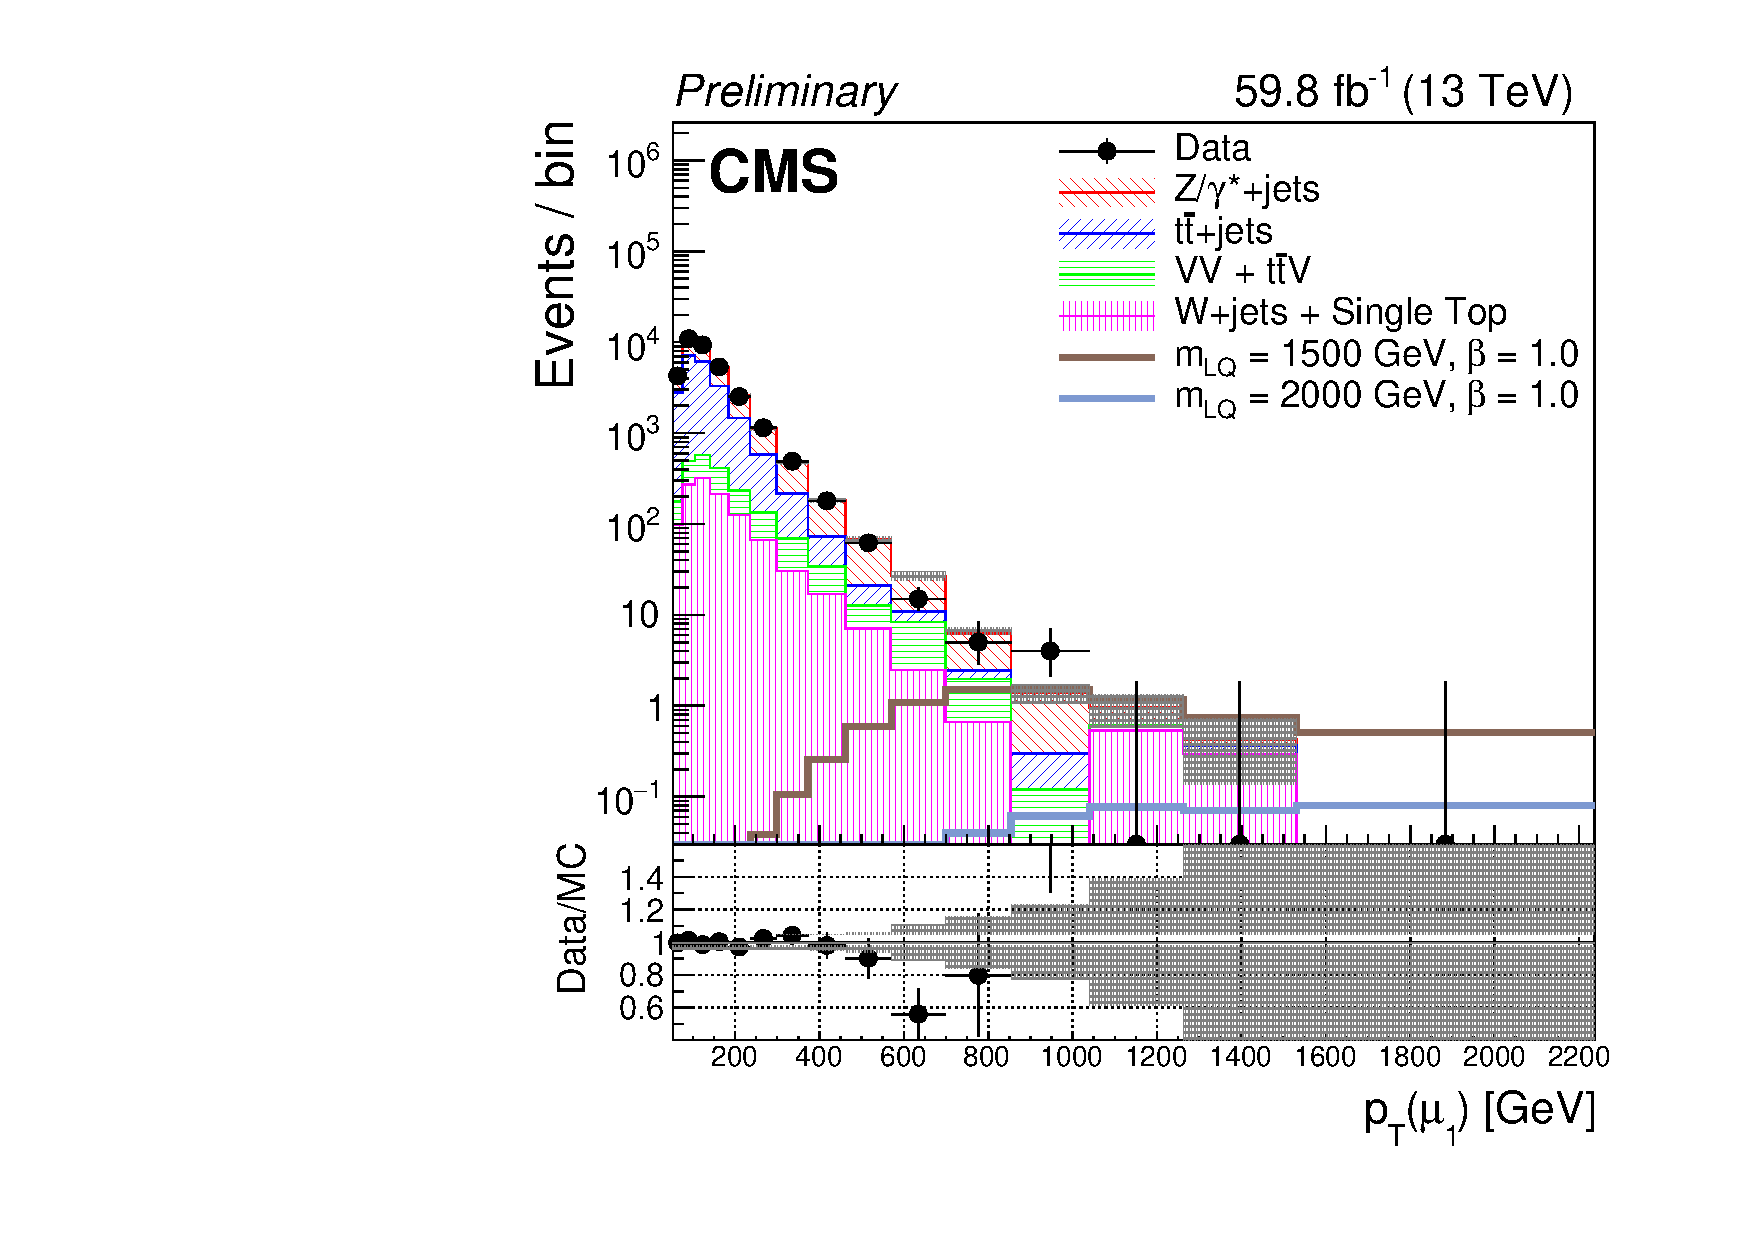
\includegraphics[width=.32\textwidth]{Images/Analysis/Results_2018_Unblinded/Plots/Preselection/BasicLQ_uujj_Pt_muon1_standard.pdf}}
       {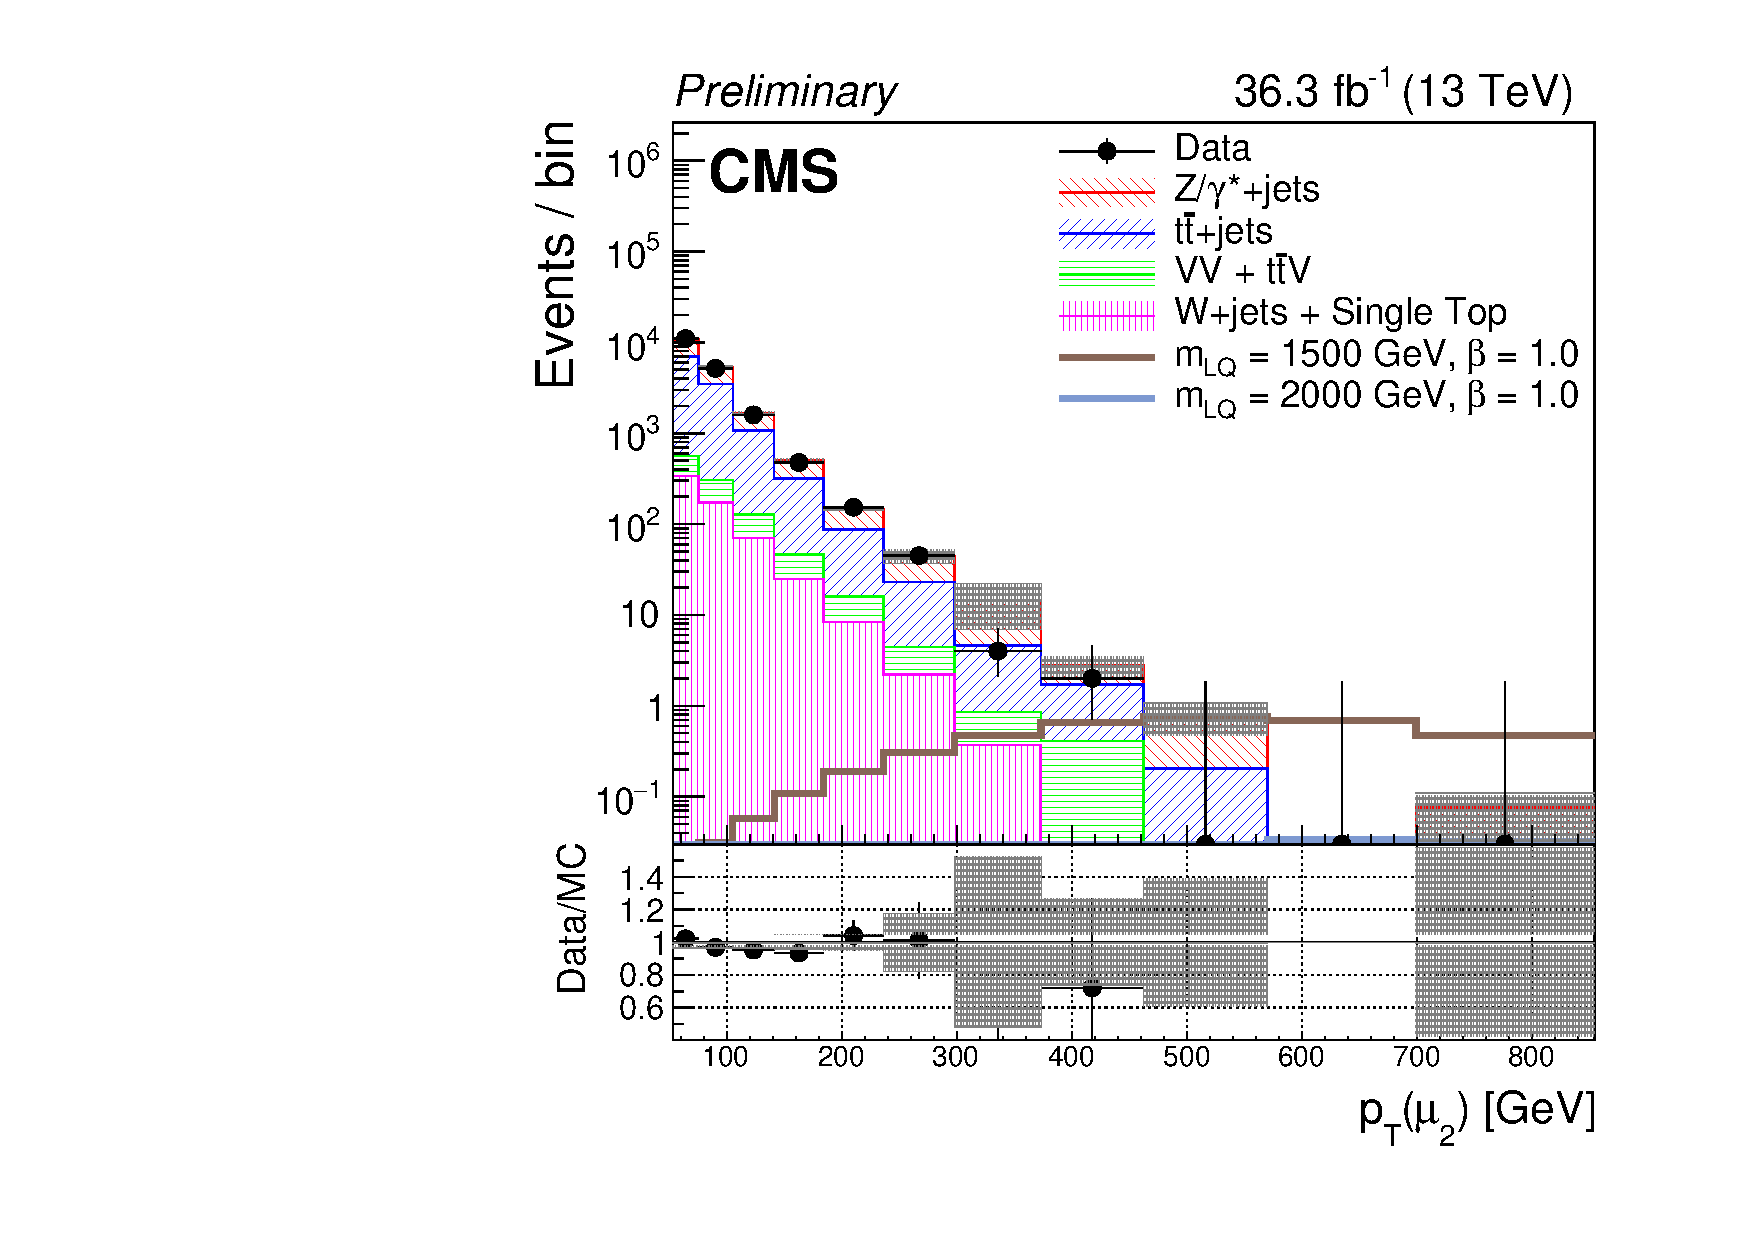
\includegraphics[width=.32\textwidth]{Images/Analysis/Results_2016_Unblinded/Plots/Preselection/BasicLQ_uujj_Pt_muon2_standard.pdf}}
       {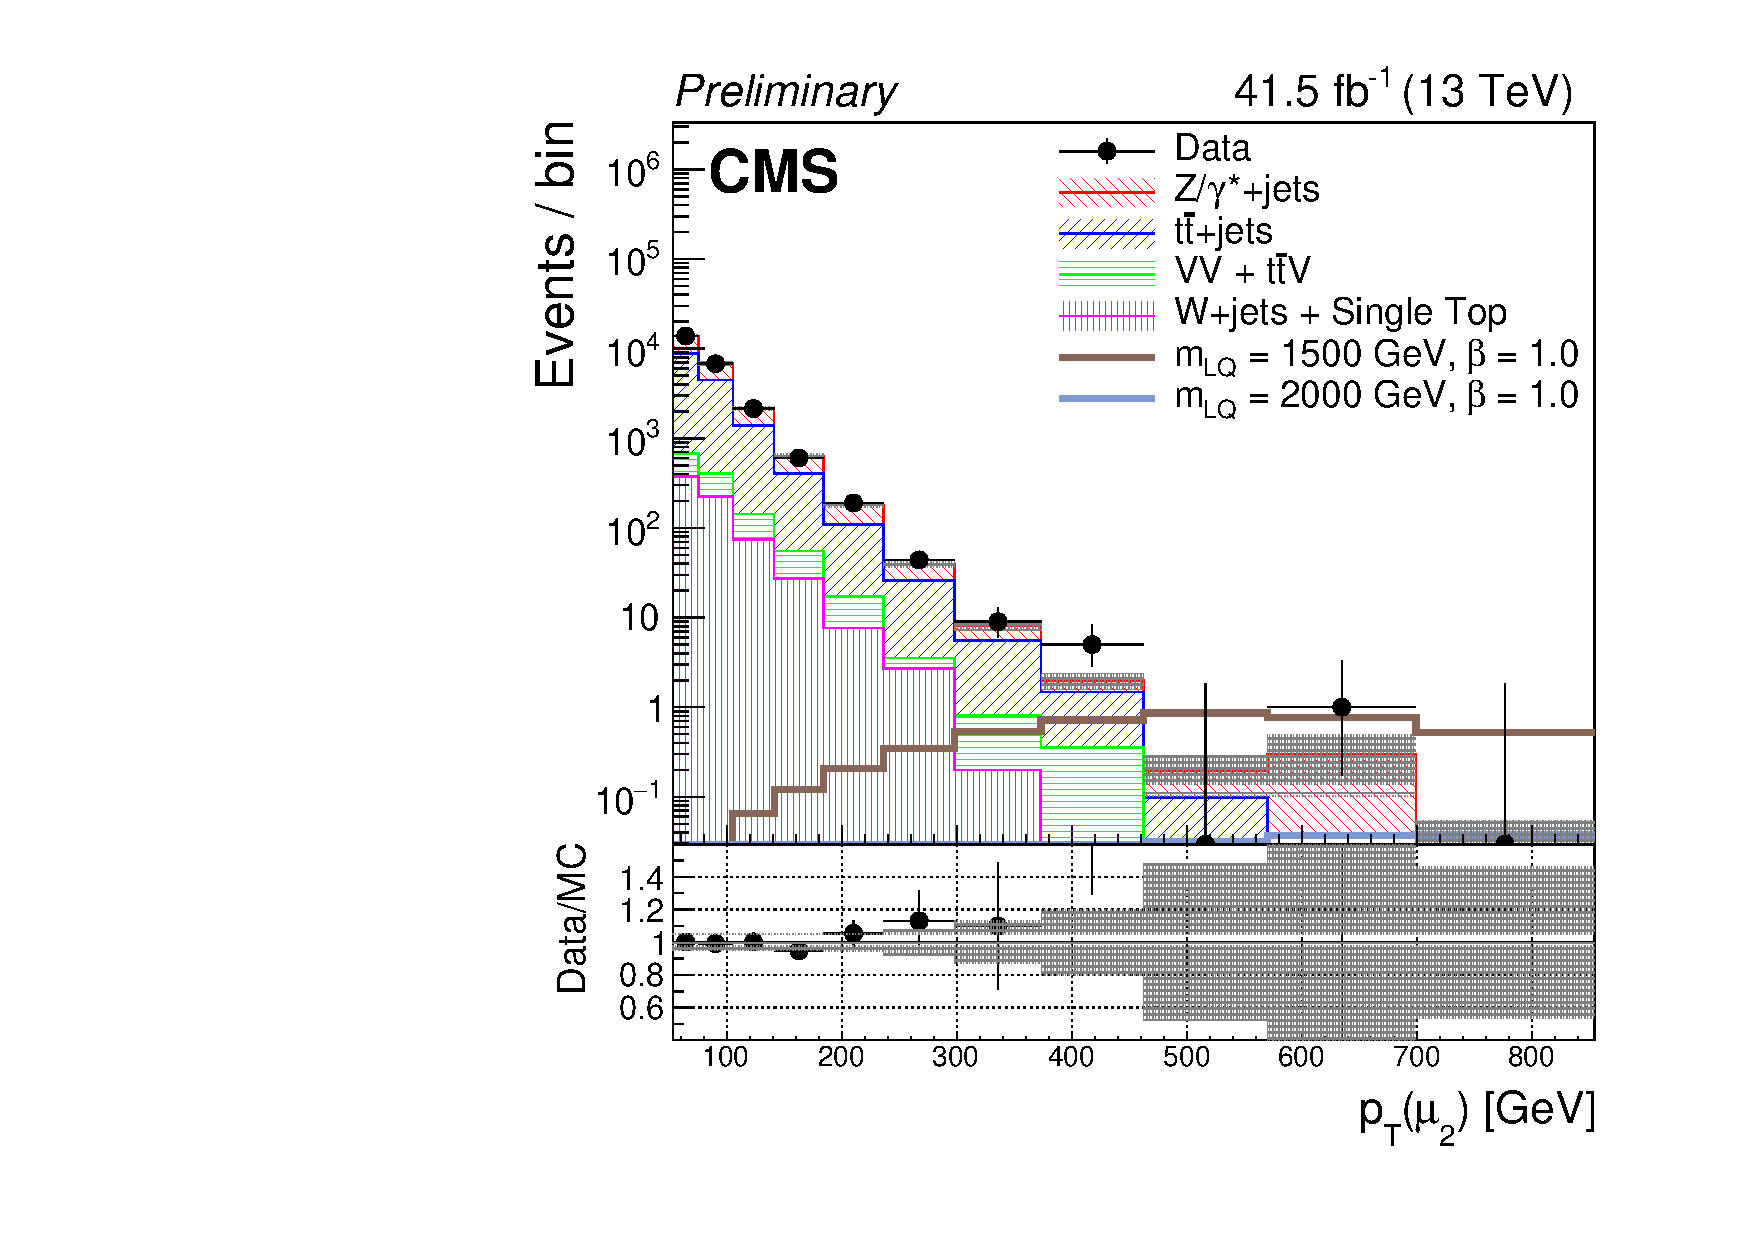
\includegraphics[width=.32\textwidth]{Images/Analysis/Results_2017_Unblinded/Plots/Preselection/BasicLQ_uujj_Pt_muon2_standard.pdf}}
       {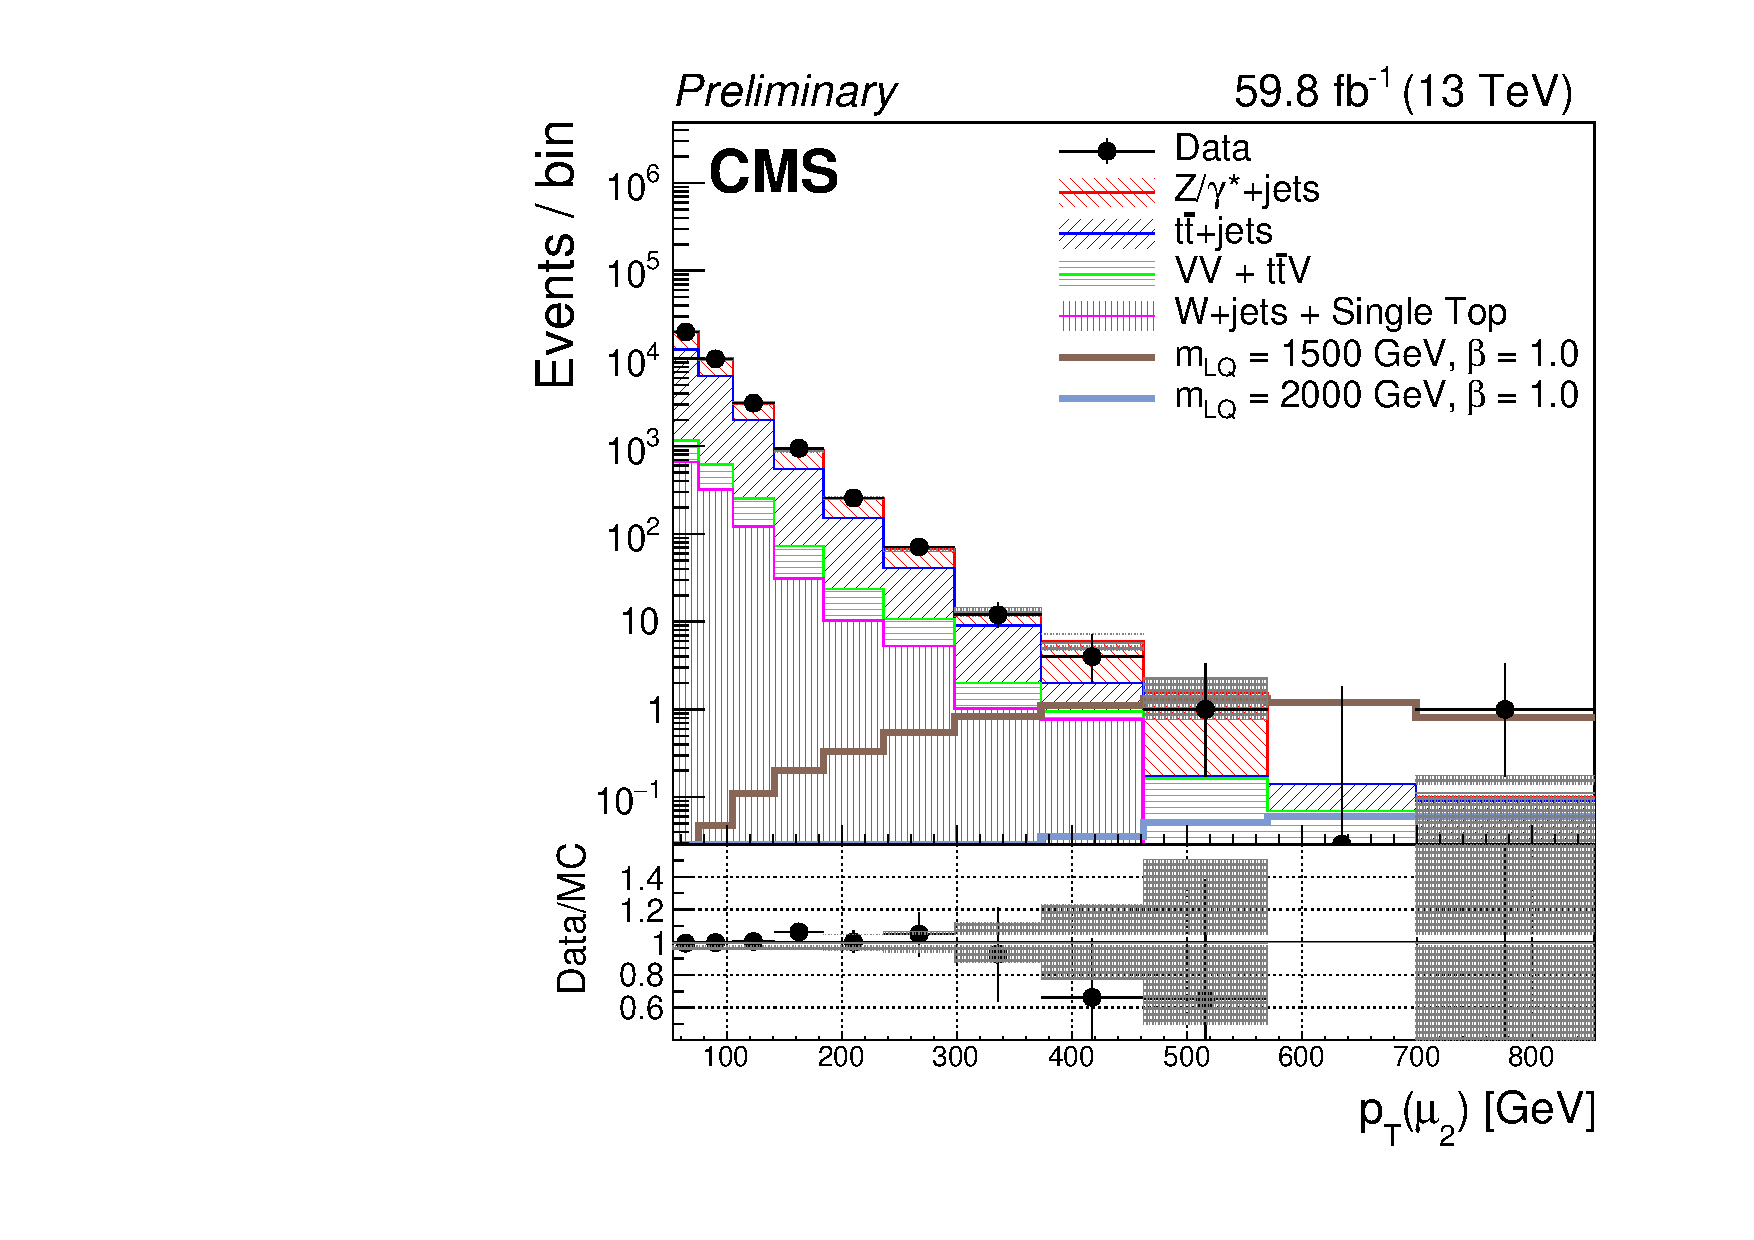
\includegraphics[width=.32\textwidth]{Images/Analysis/Results_2018_Unblinded/Plots/Preselection/BasicLQ_uujj_Pt_muon2_standard.pdf}}
       {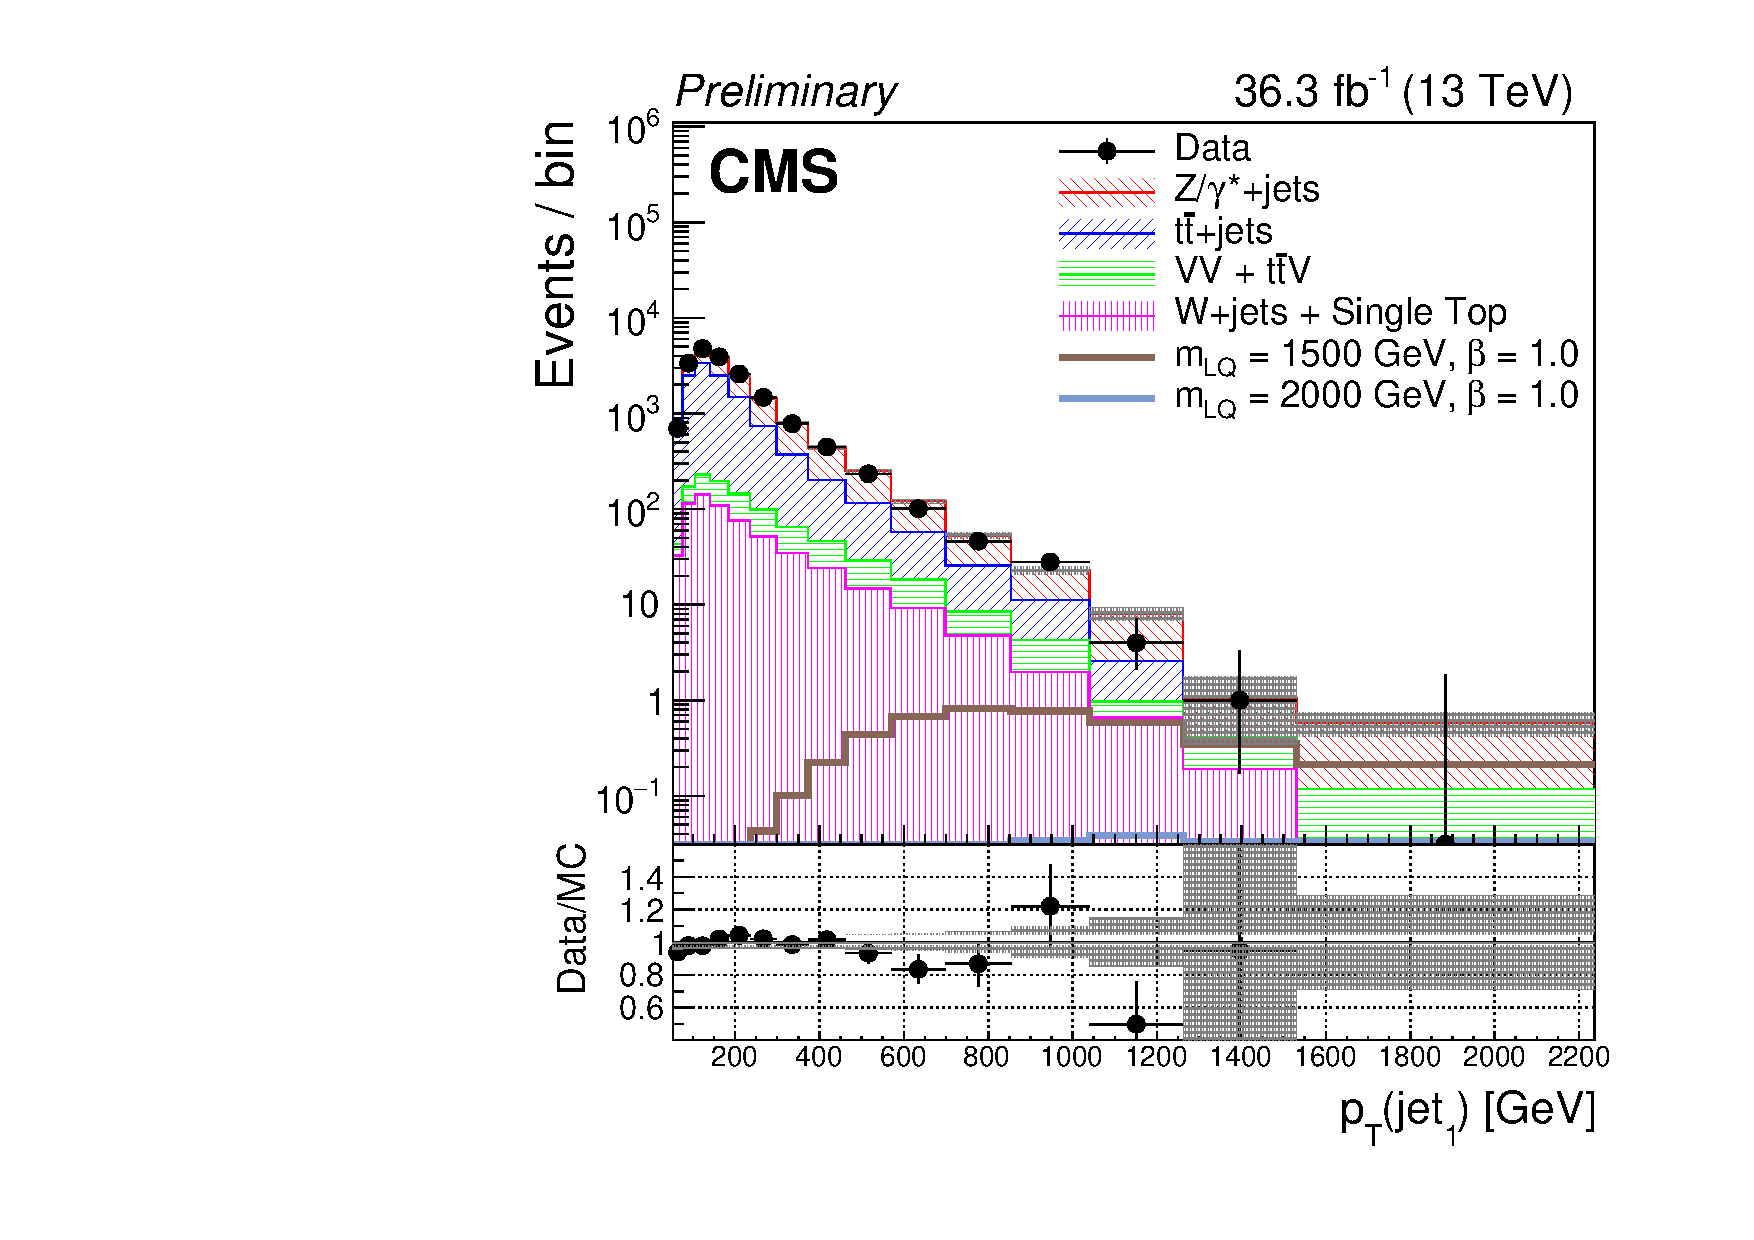
\includegraphics[width=.32\textwidth]{Images/Analysis/Results_2016_Unblinded/Plots/Preselection/BasicLQ_uujj_Pt_jet1_standard.pdf}}
       {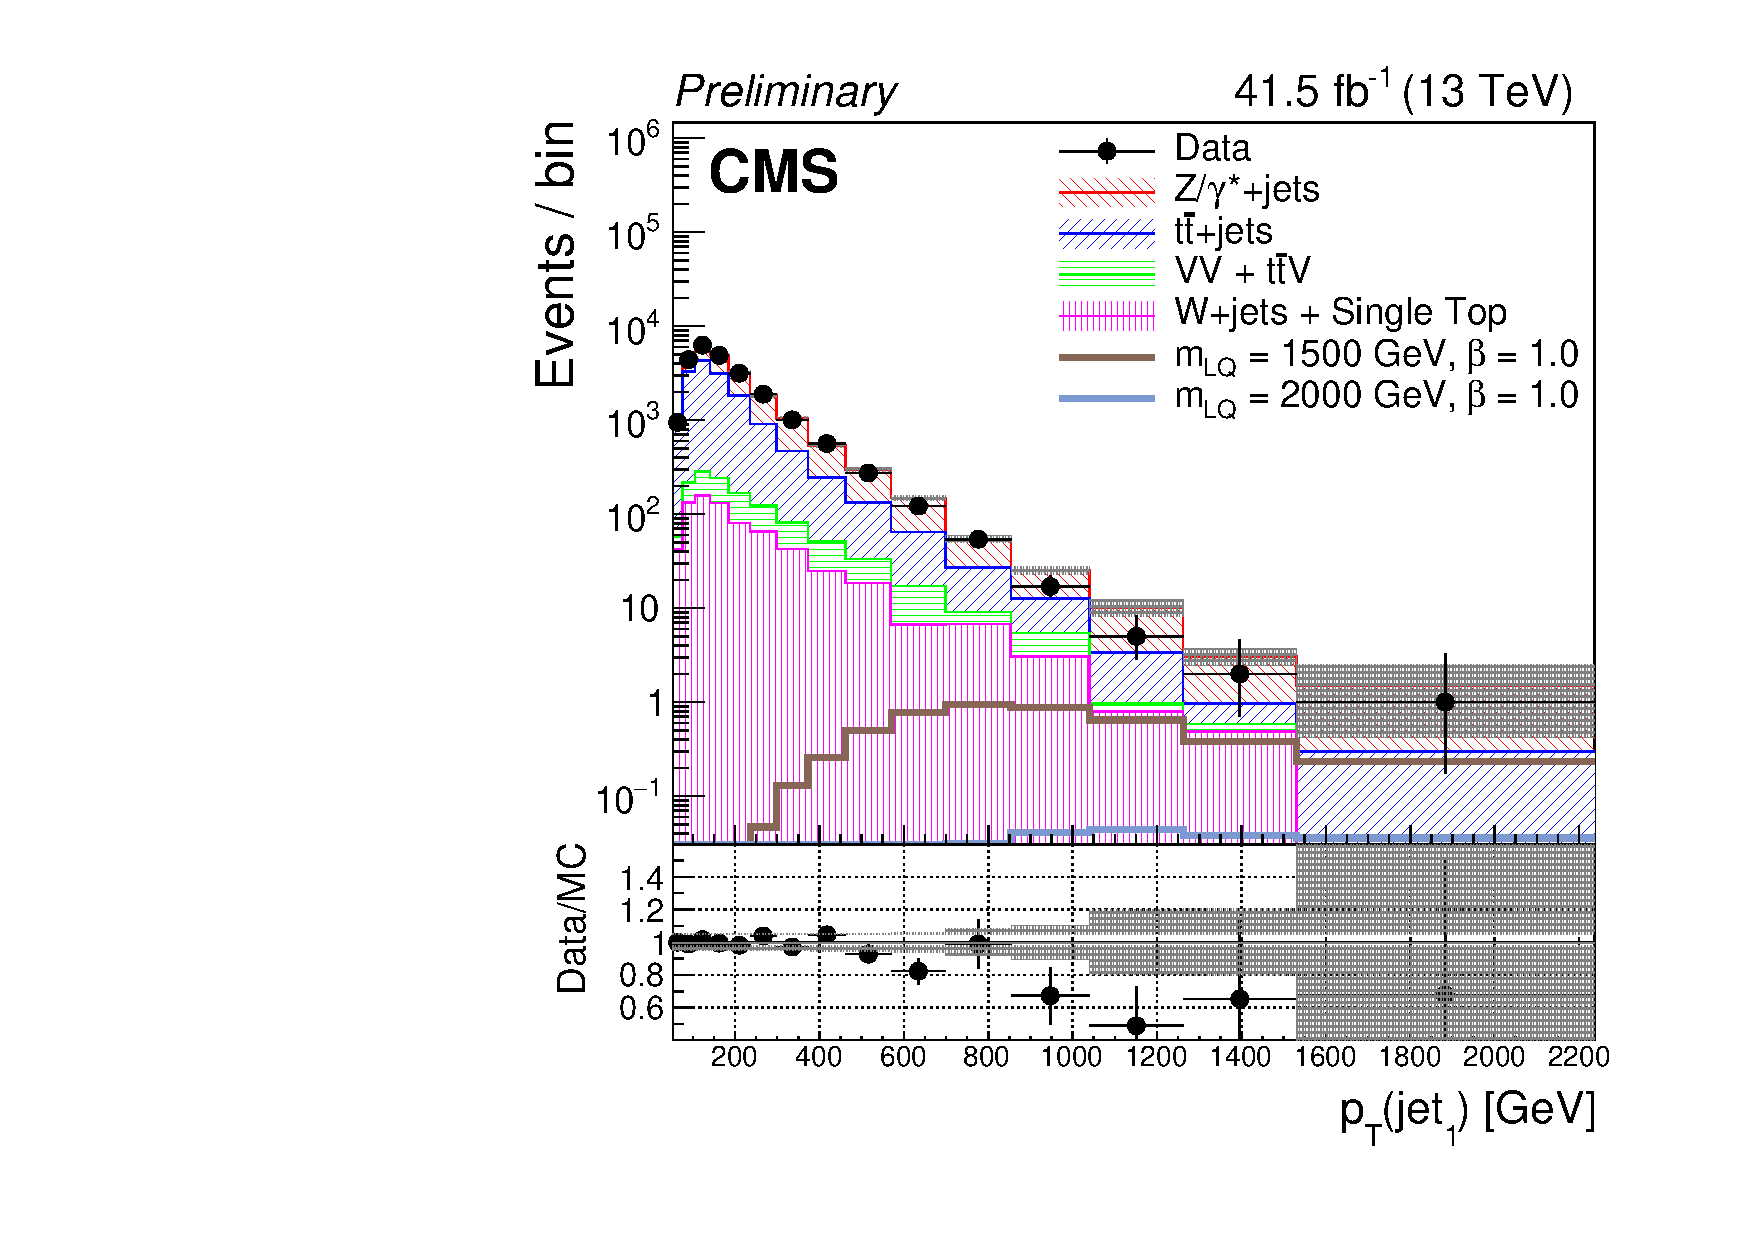
\includegraphics[width=.32\textwidth]{Images/Analysis/Results_2017_Unblinded/Plots/Preselection/BasicLQ_uujj_Pt_jet1_standard.pdf}}
       {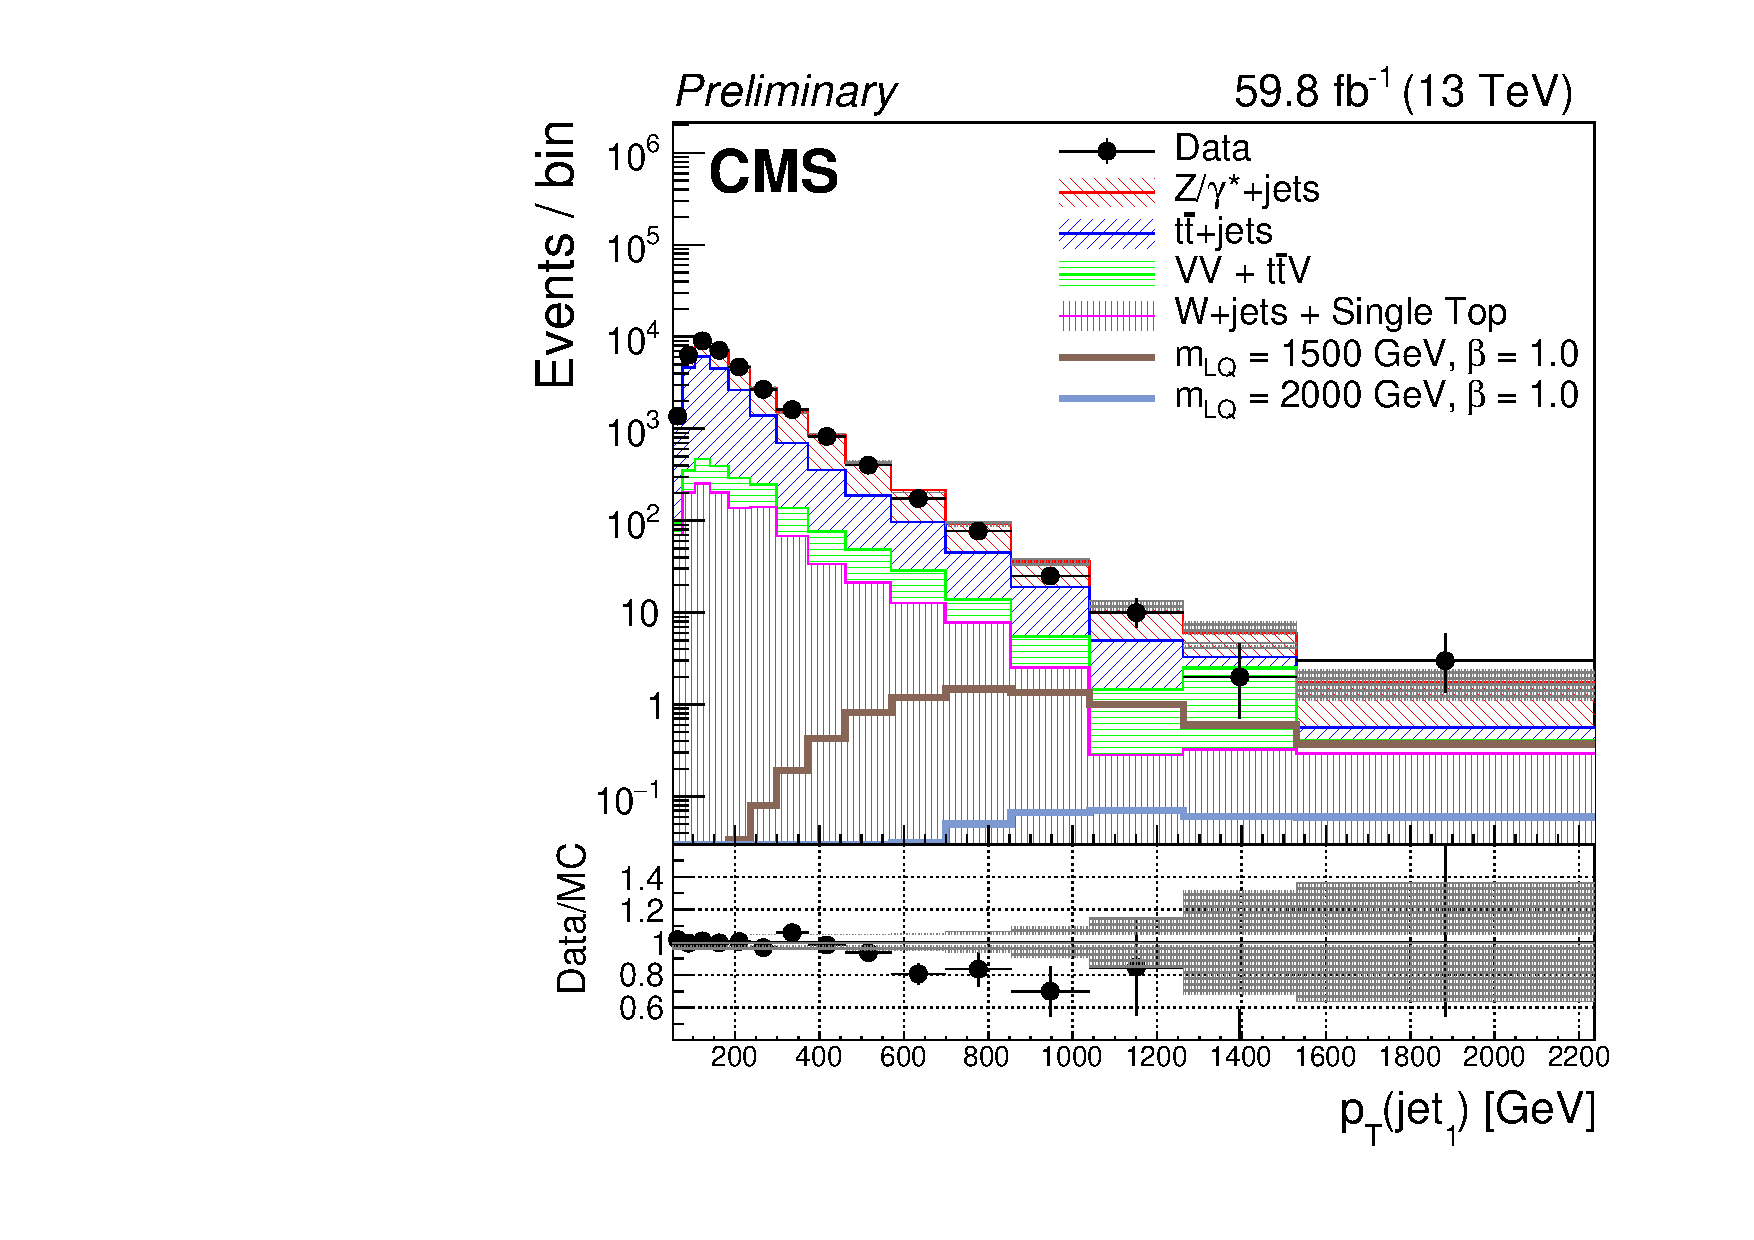
\includegraphics[width=.32\textwidth]{Images/Analysis/Results_2018_Unblinded/Plots/Preselection/BasicLQ_uujj_Pt_jet1_standard.pdf}}
       {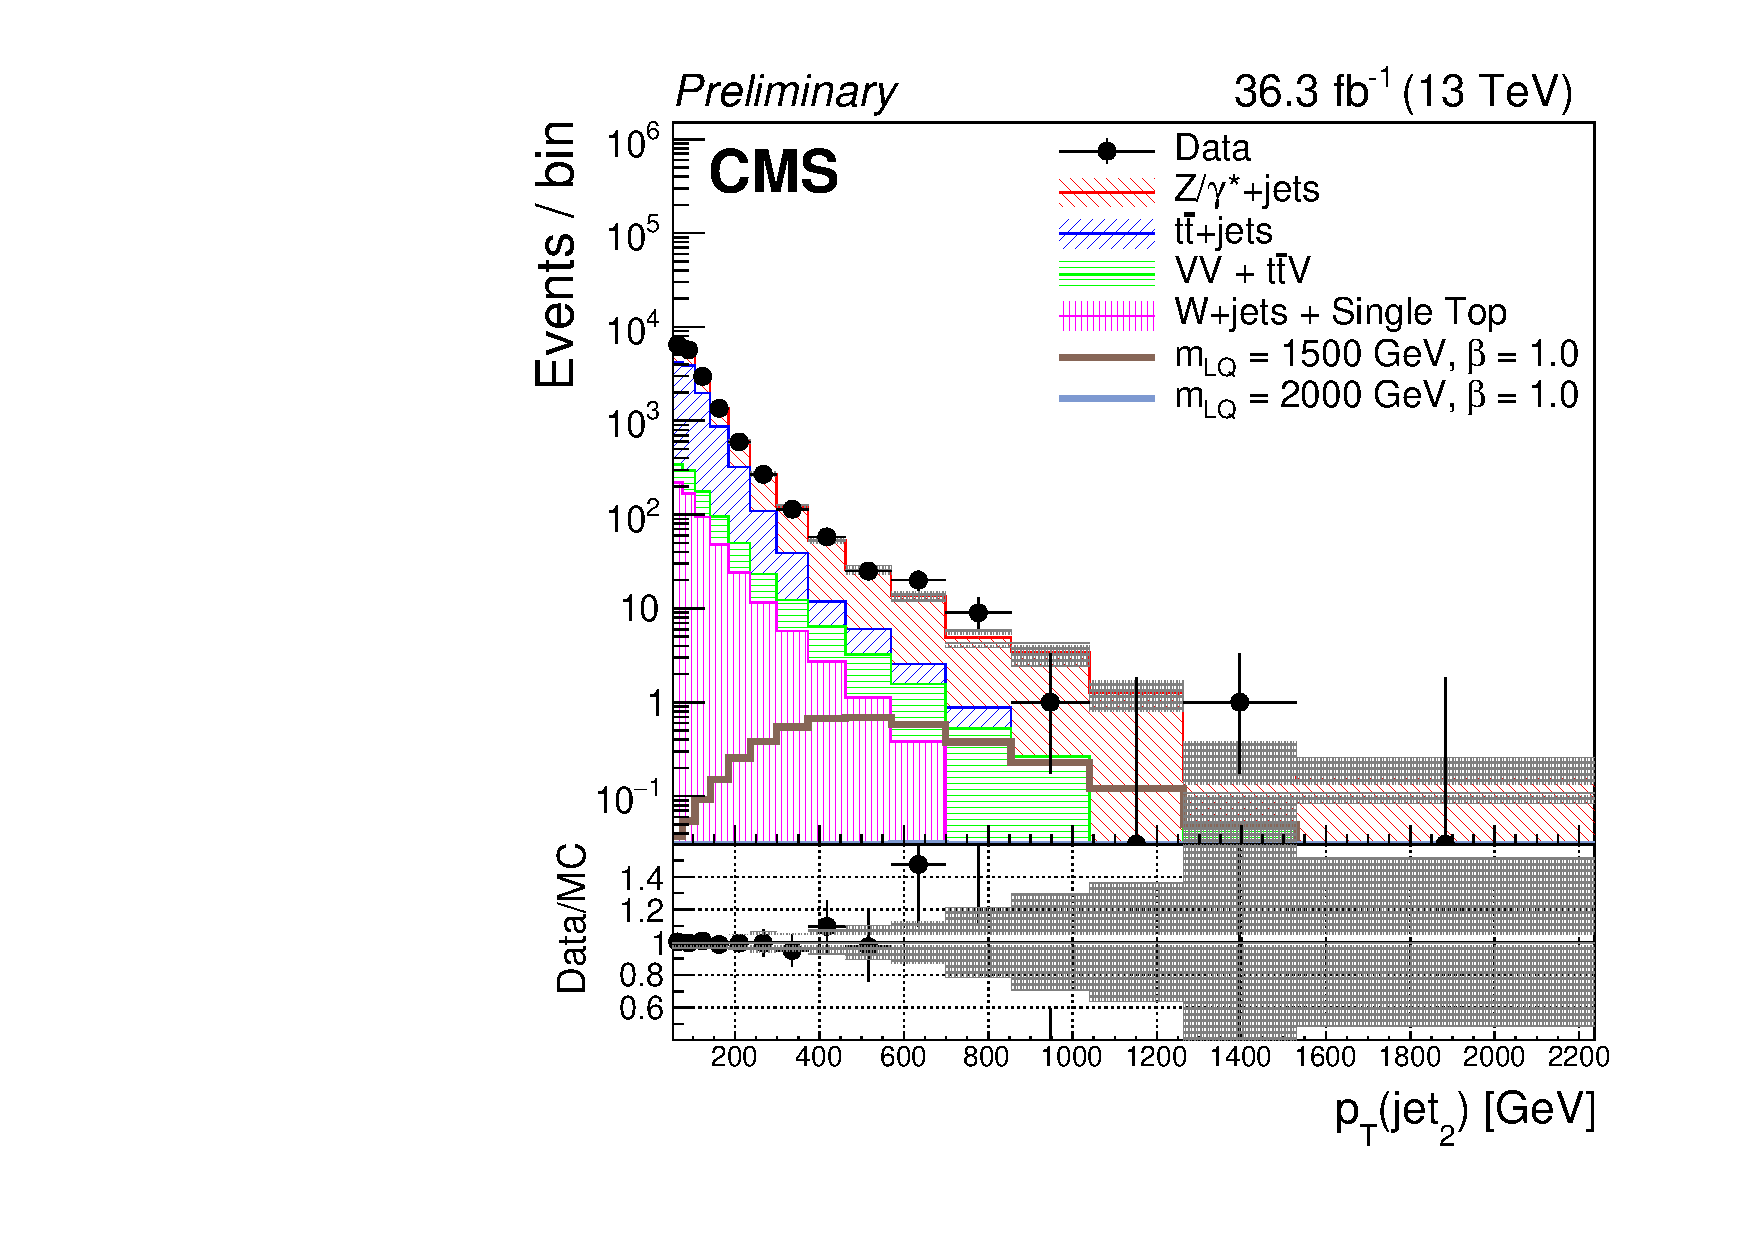
\includegraphics[width=.32\textwidth]{Images/Analysis/Results_2016_Unblinded/Plots/Preselection/BasicLQ_uujj_Pt_jet2_standard.pdf}}
       {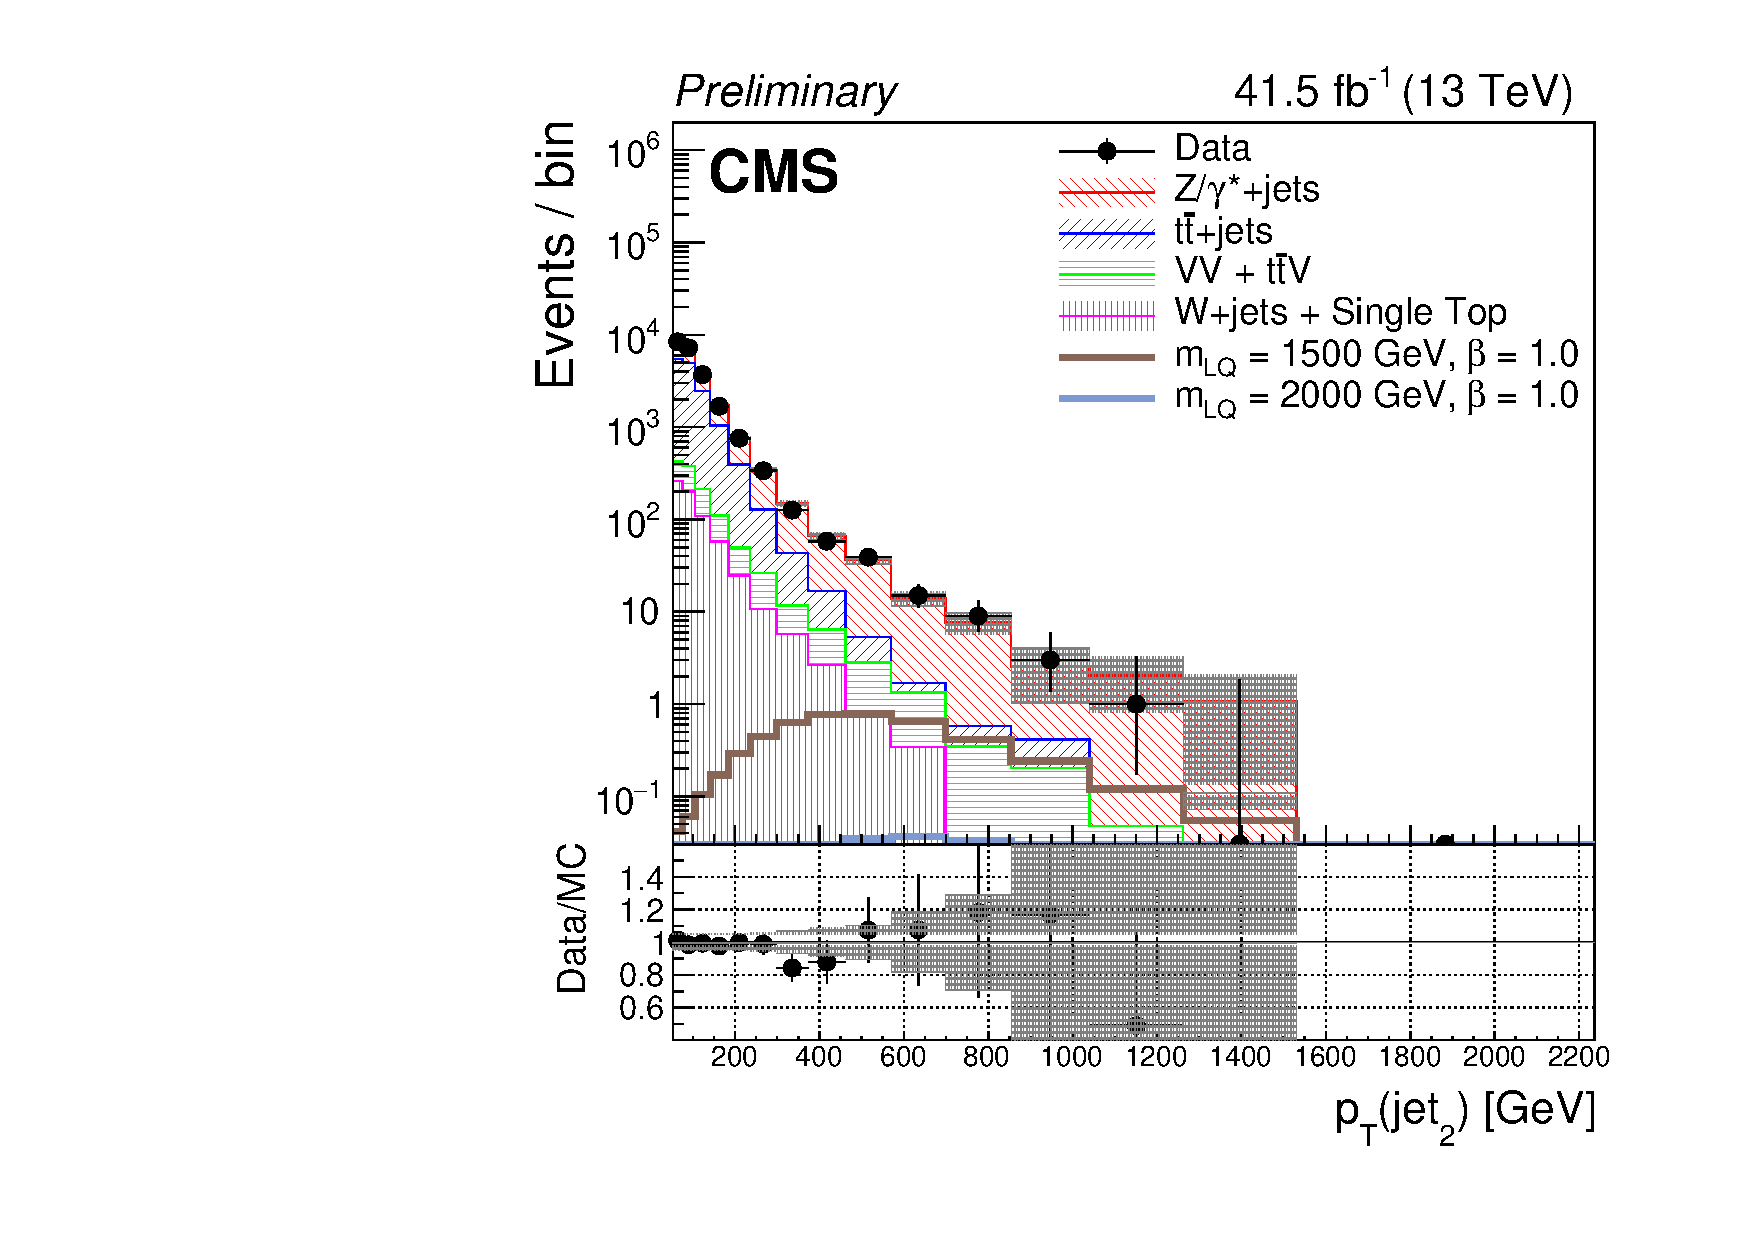
\includegraphics[width=.32\textwidth]{Images/Analysis/Results_2017_Unblinded/Plots/Preselection/BasicLQ_uujj_Pt_jet2_standard.pdf}}
       {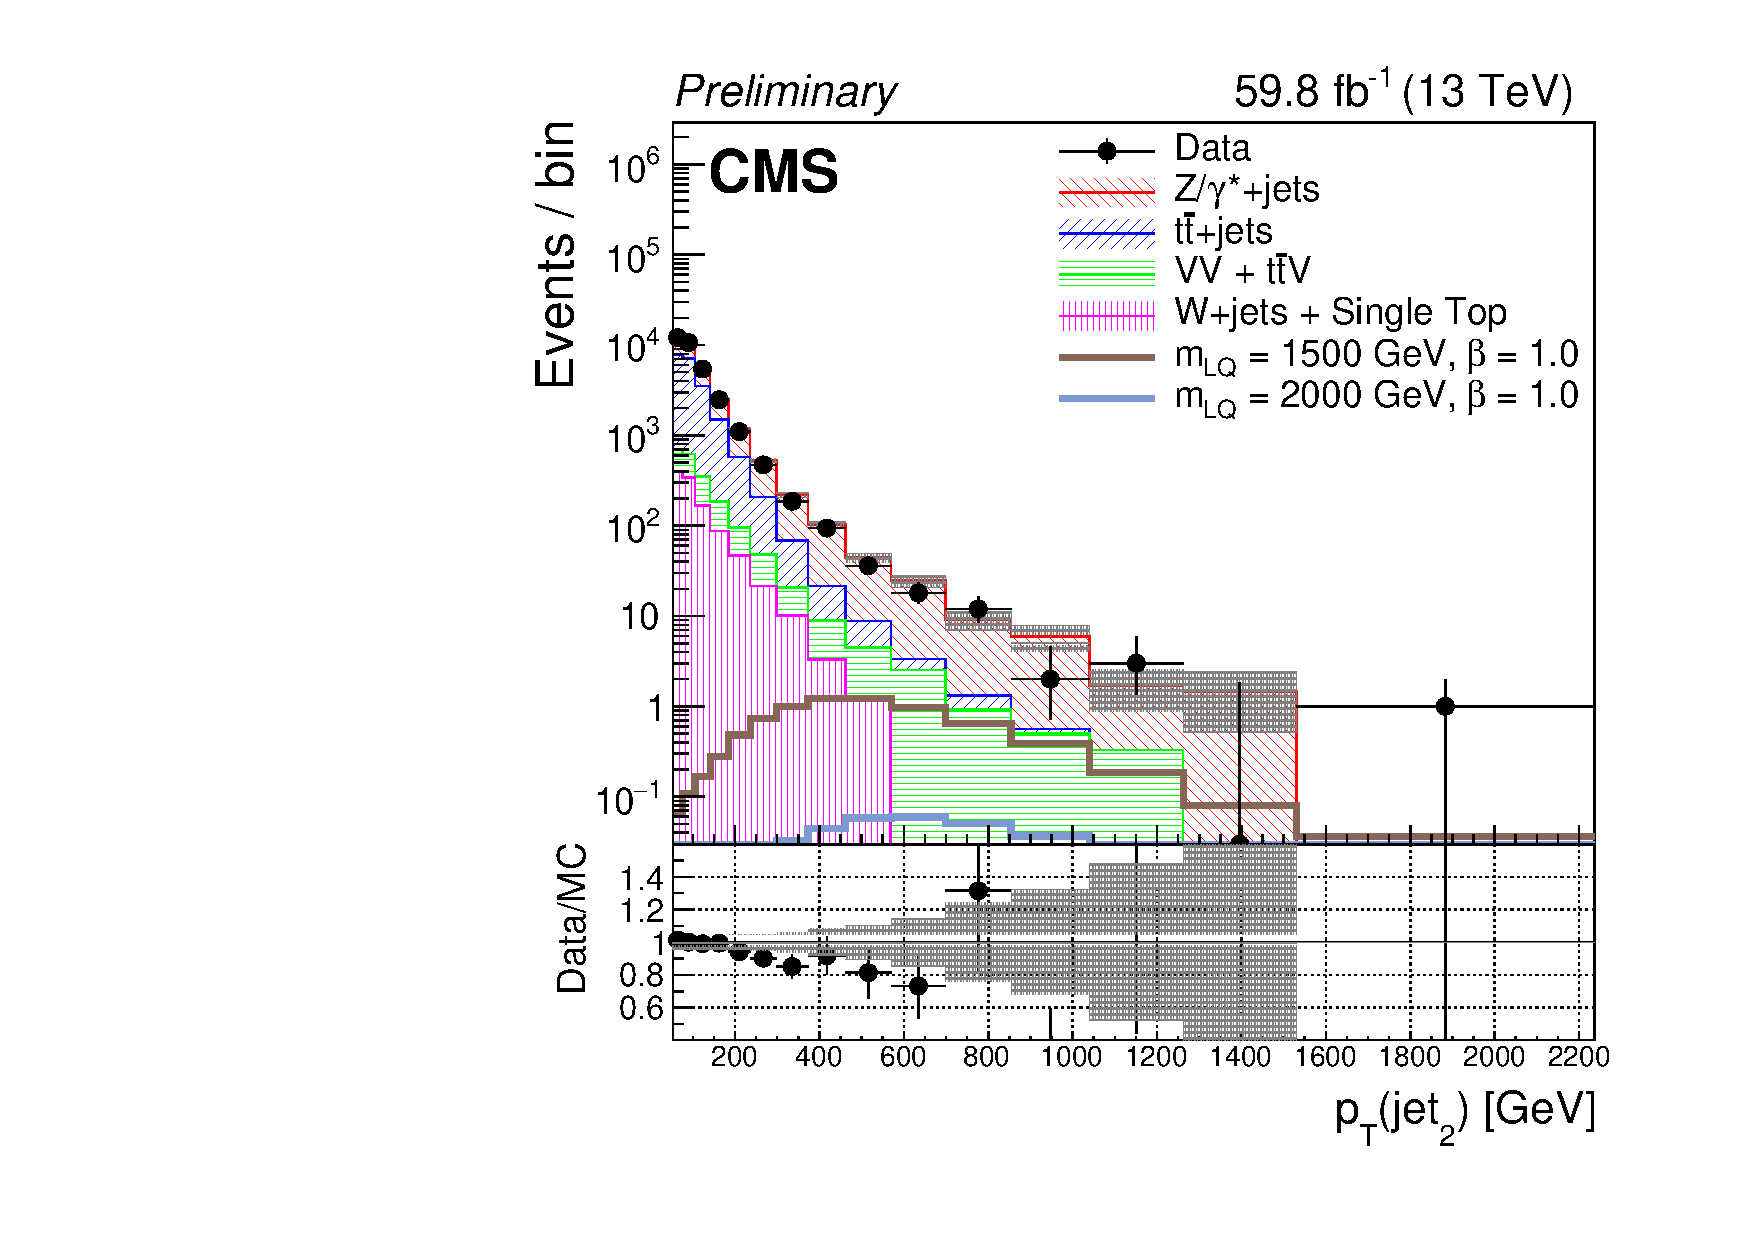
\includegraphics[width=.32\textwidth]{Images/Analysis/Results_2018_Unblinded/Plots/Preselection/BasicLQ_uujj_Pt_jet2_standard.pdf}}
       \caption{A comparison between distributions of observed data and SM expectation at preselection level. Left to right: 2016, 2017, 2018 data. Top to bottom: muon 1 \pt, muon 2 \pt, jet 1 \pt, and jet 2 \pt. Error bars on observed data points represent statistical uncertainties, and systematic uncertainties on SM expectation are shown by gray hashing.}
	\label{figapp:preselpt}
\end{figure}

\begin{figure}[H]
       \centering
       {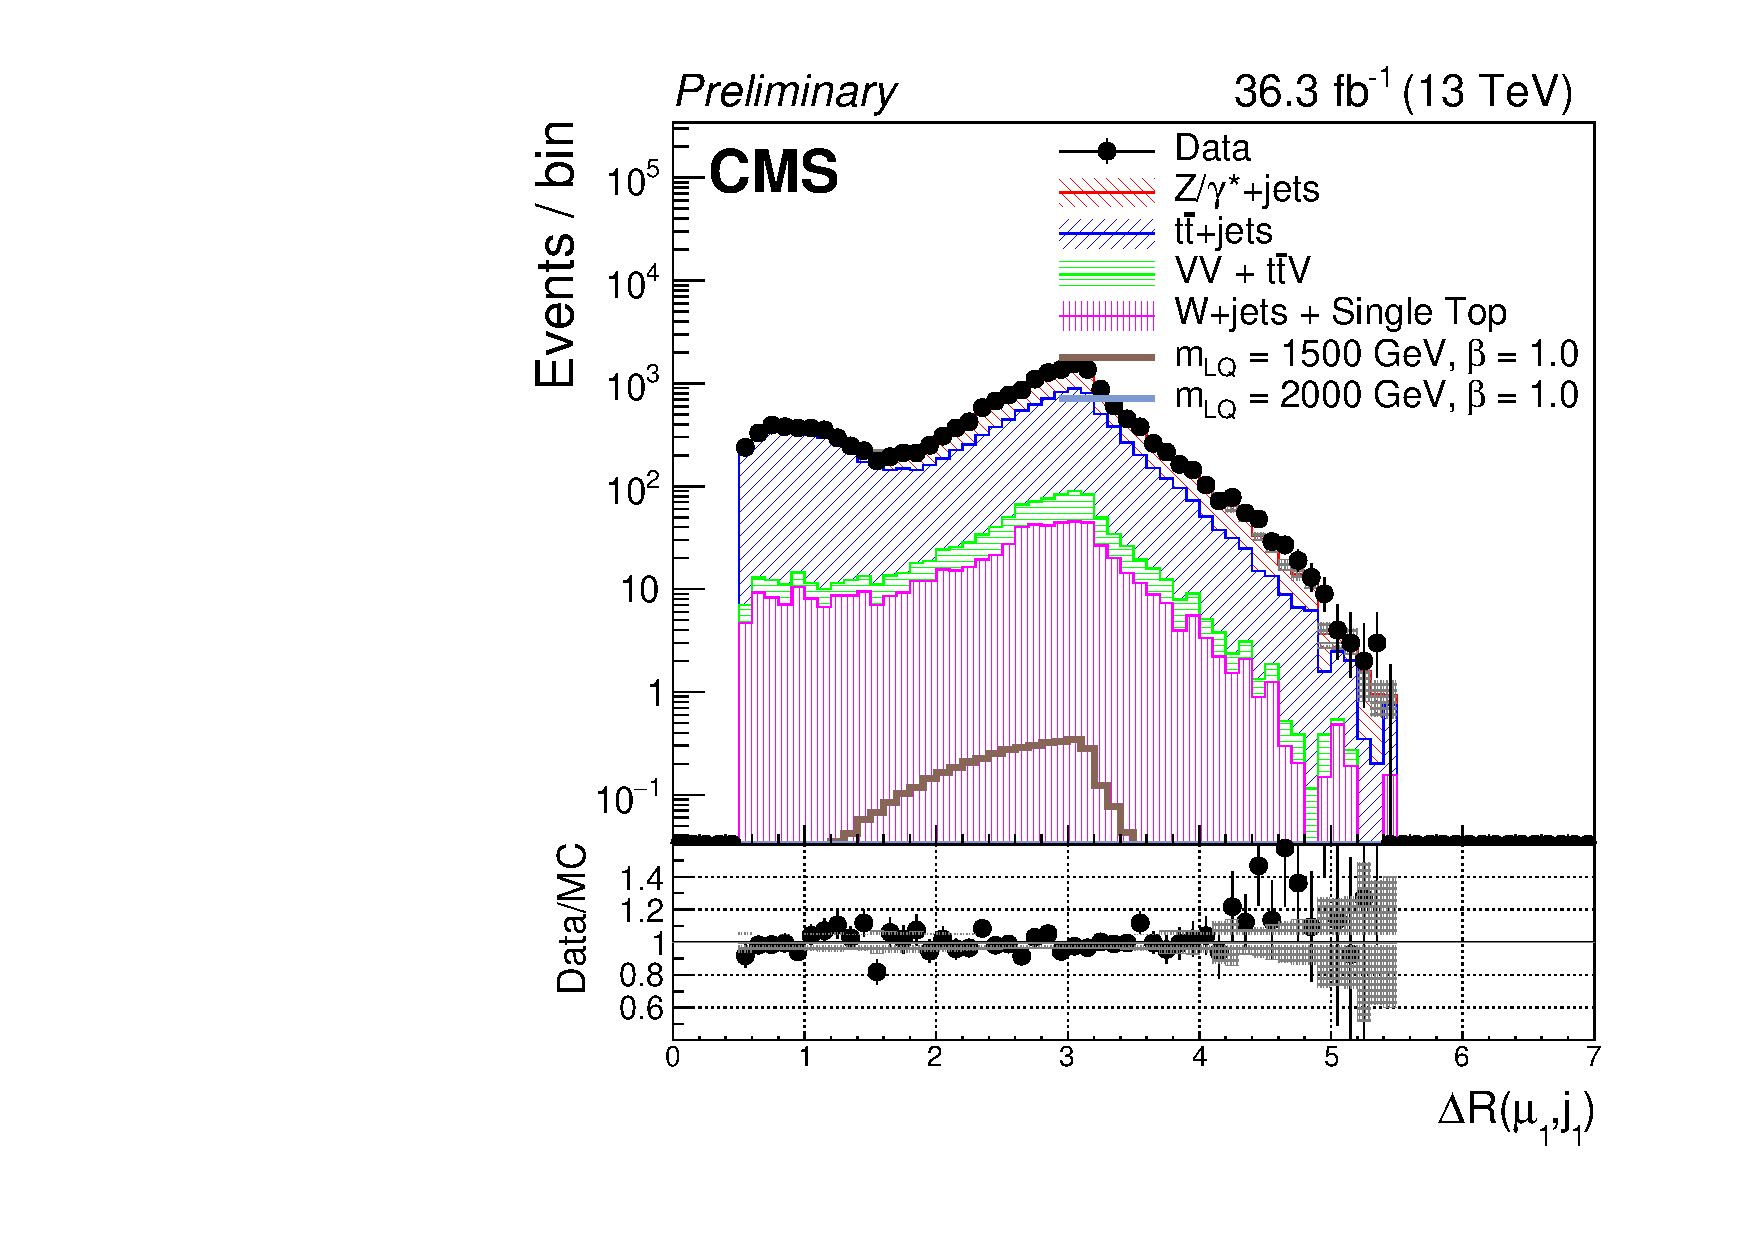
\includegraphics[width=0.32\textwidth]{Images/Analysis/Results_2016_Unblinded/Plots/Preselection/BasicLQ_uujj_DR_muon1jet1_standard.pdf}}
       {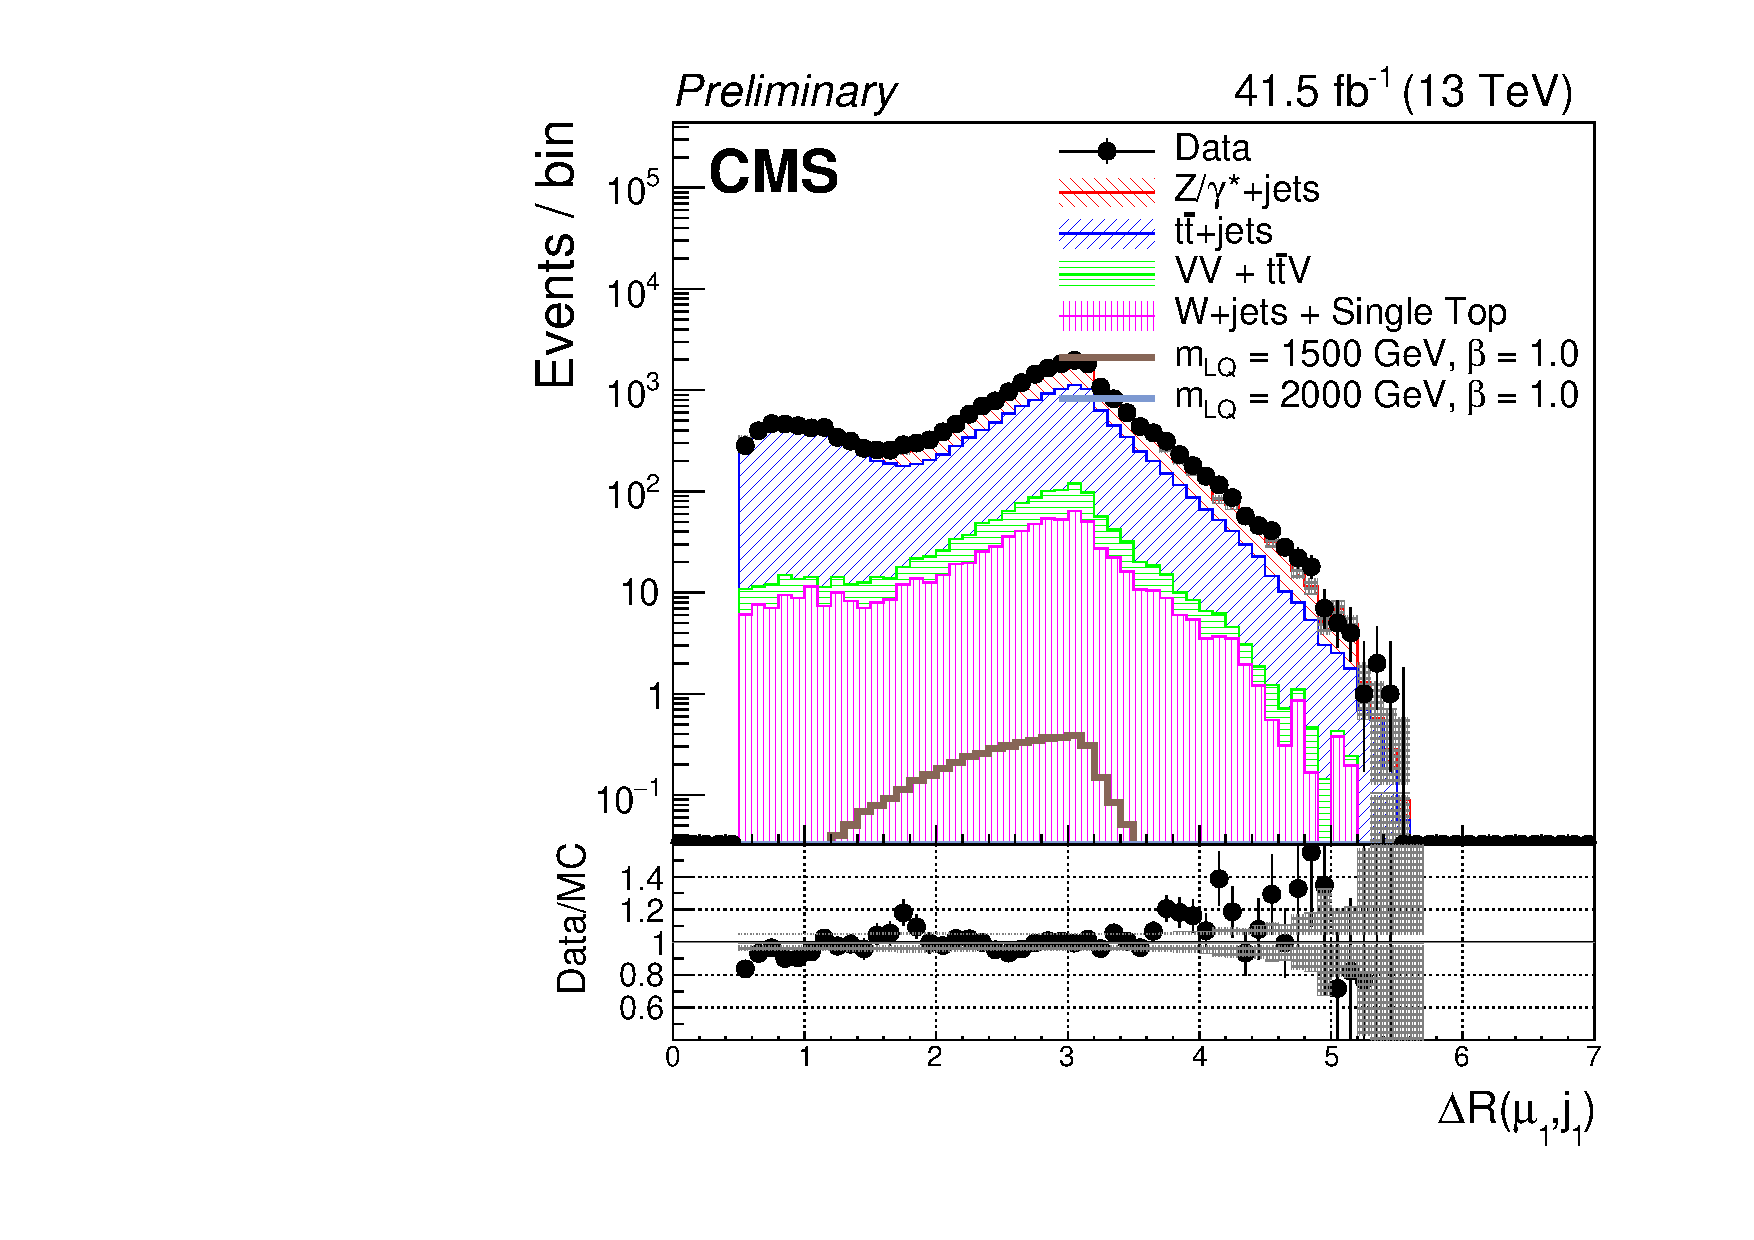
\includegraphics[width=0.32\textwidth]{Images/Analysis/Results_2017_Unblinded/Plots/Preselection/BasicLQ_uujj_DR_muon1jet1_standard.pdf}}
       {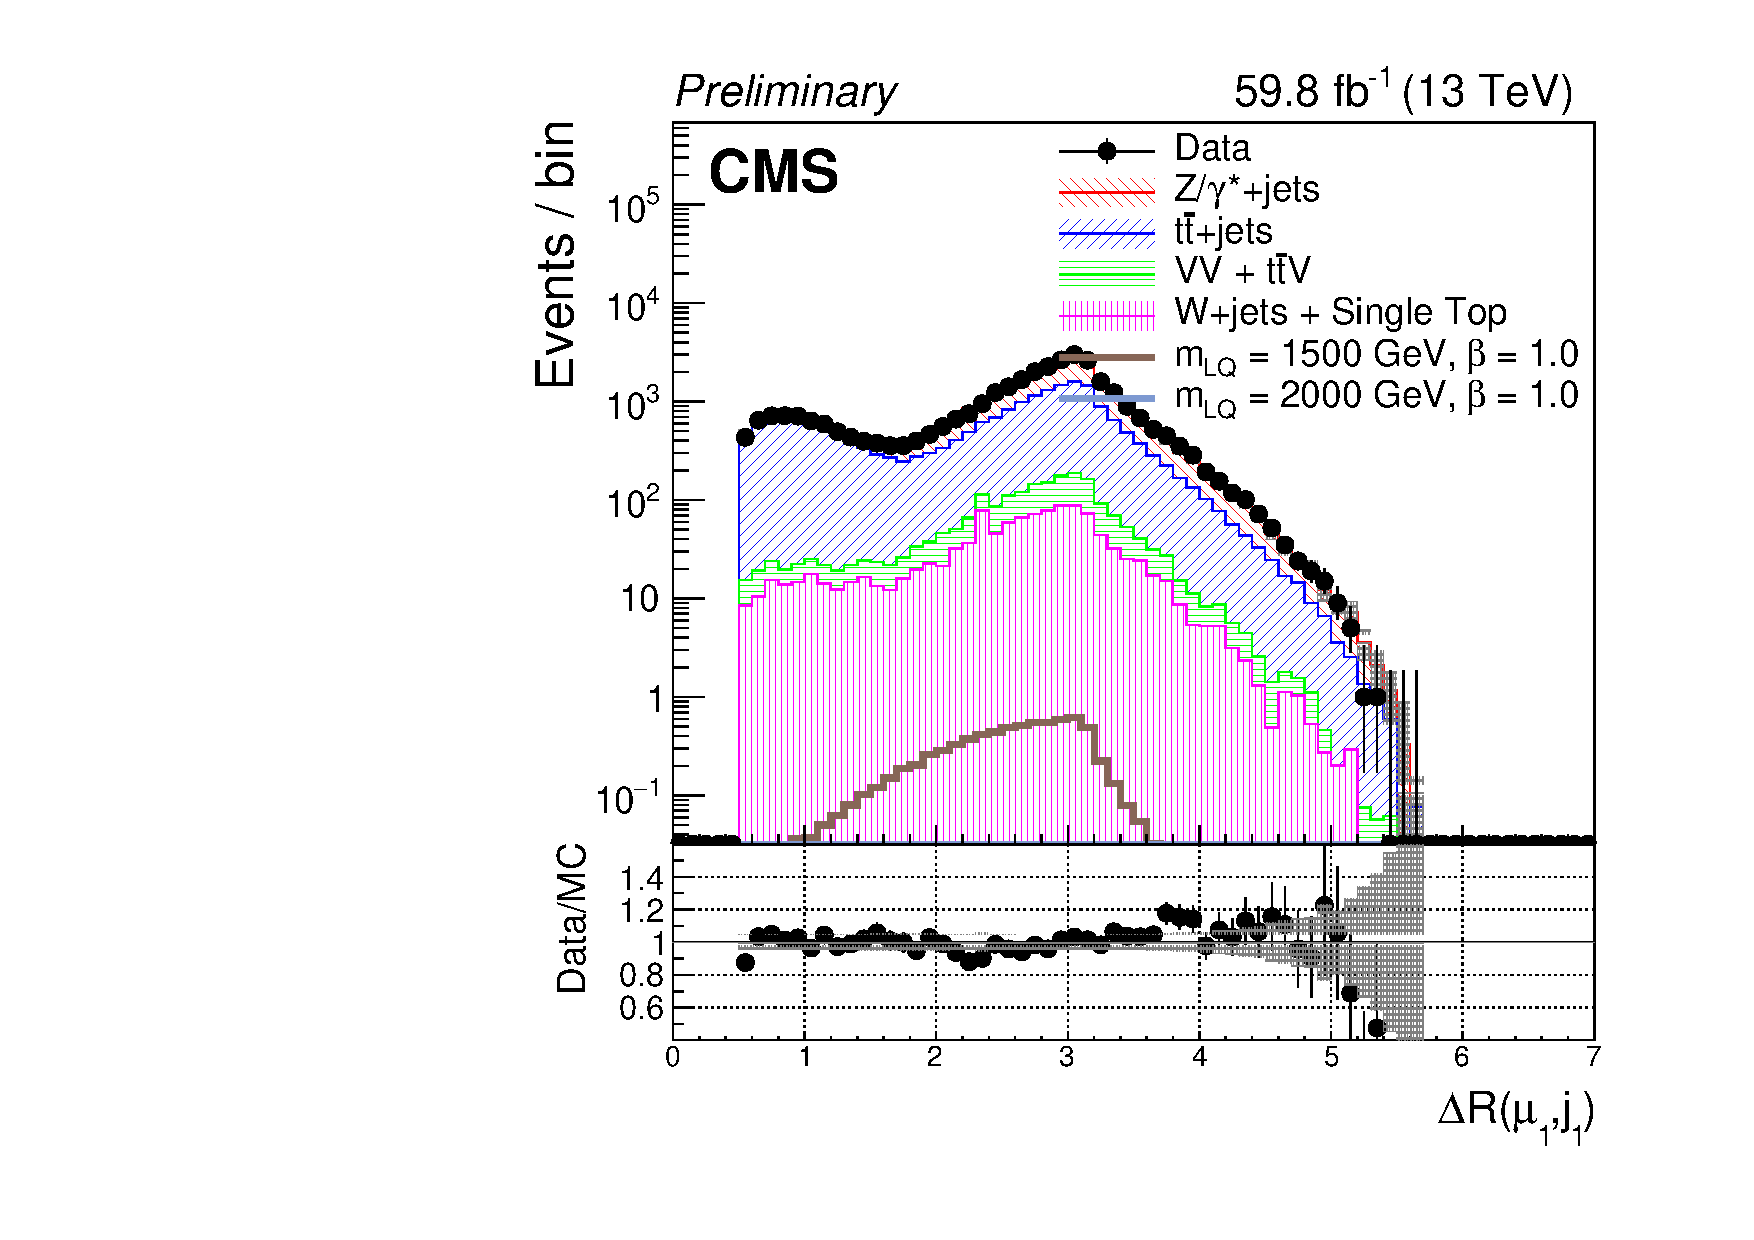
\includegraphics[width=0.32\textwidth]{Images/Analysis/Results_2018_Unblinded/Plots/Preselection/BasicLQ_uujj_DR_muon1jet1_standard.pdf}}
       {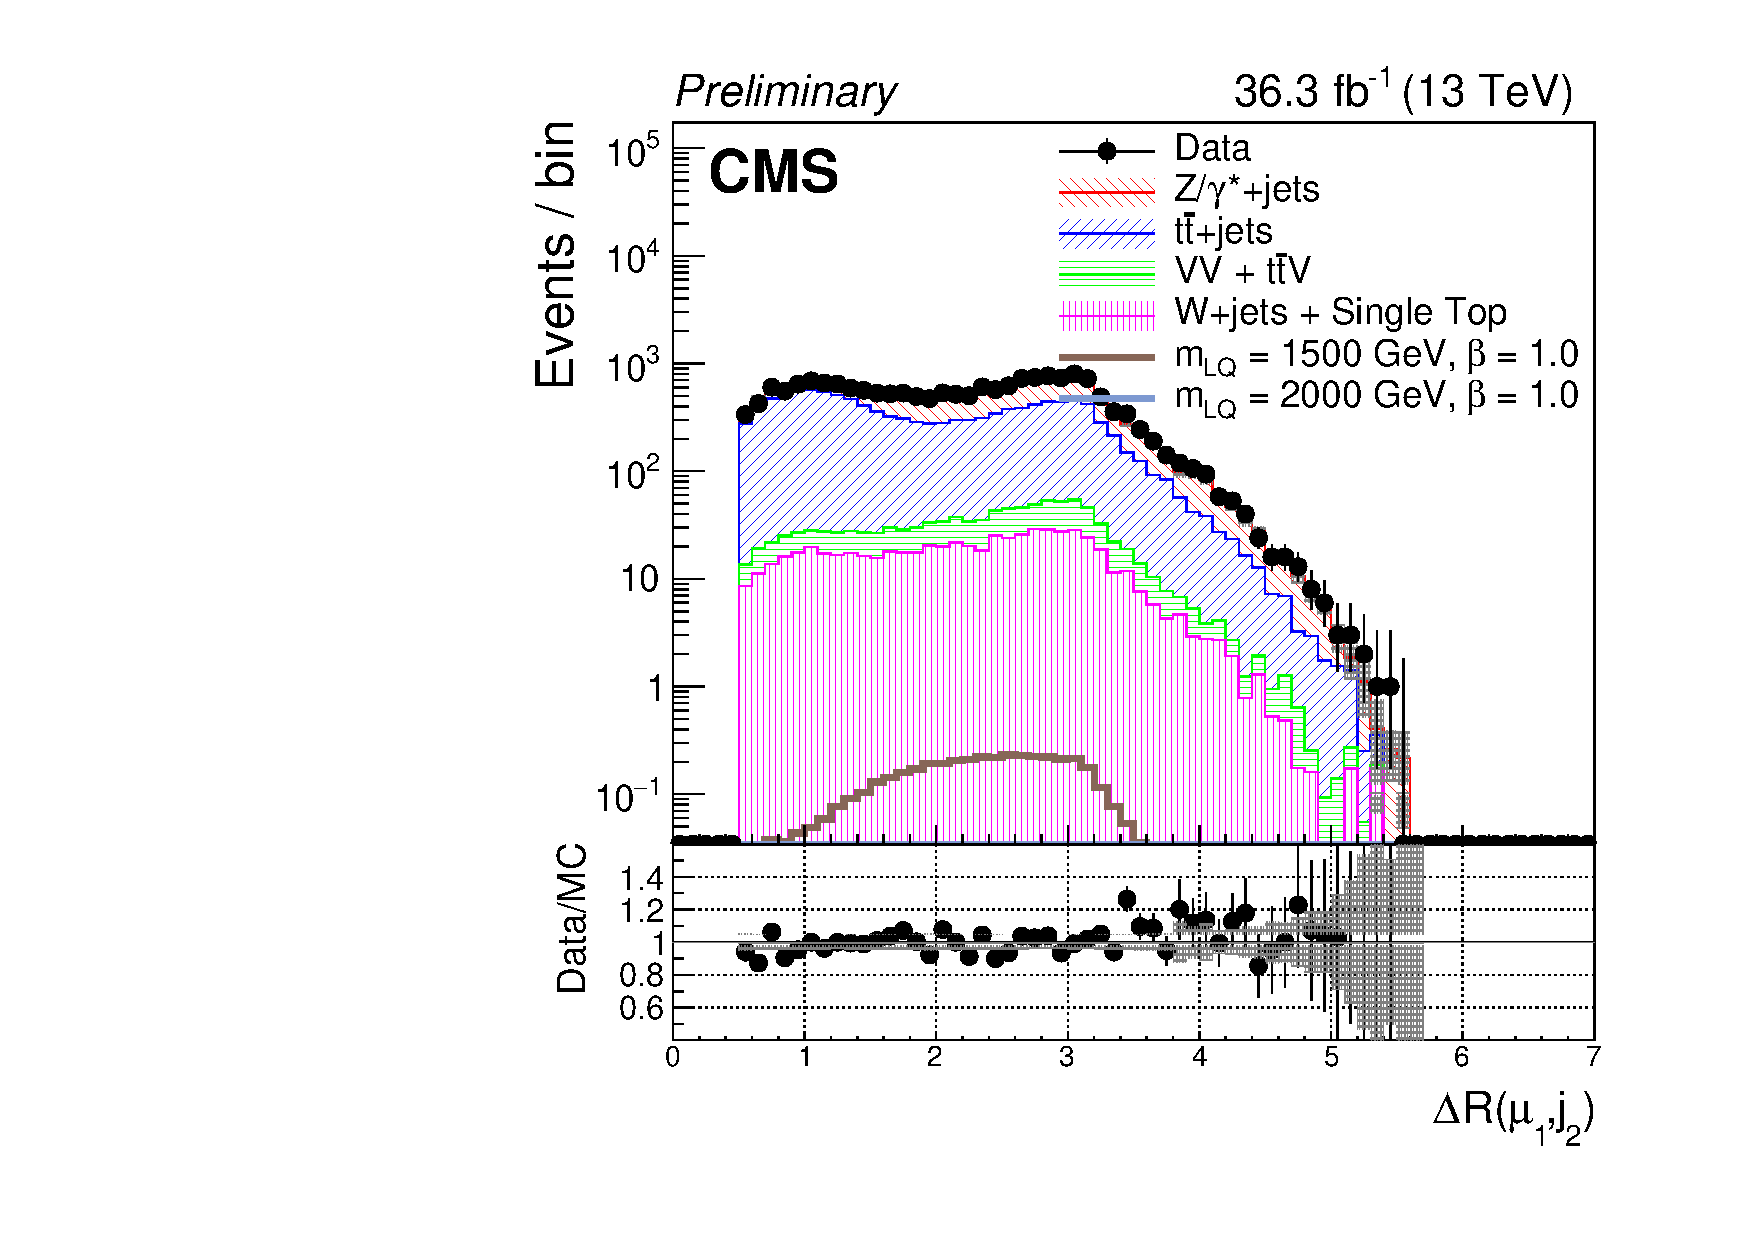
\includegraphics[width=0.32\textwidth]{Images/Analysis/Results_2016_Unblinded/Plots/Preselection/BasicLQ_uujj_DR_muon1jet2_standard.pdf}}
       {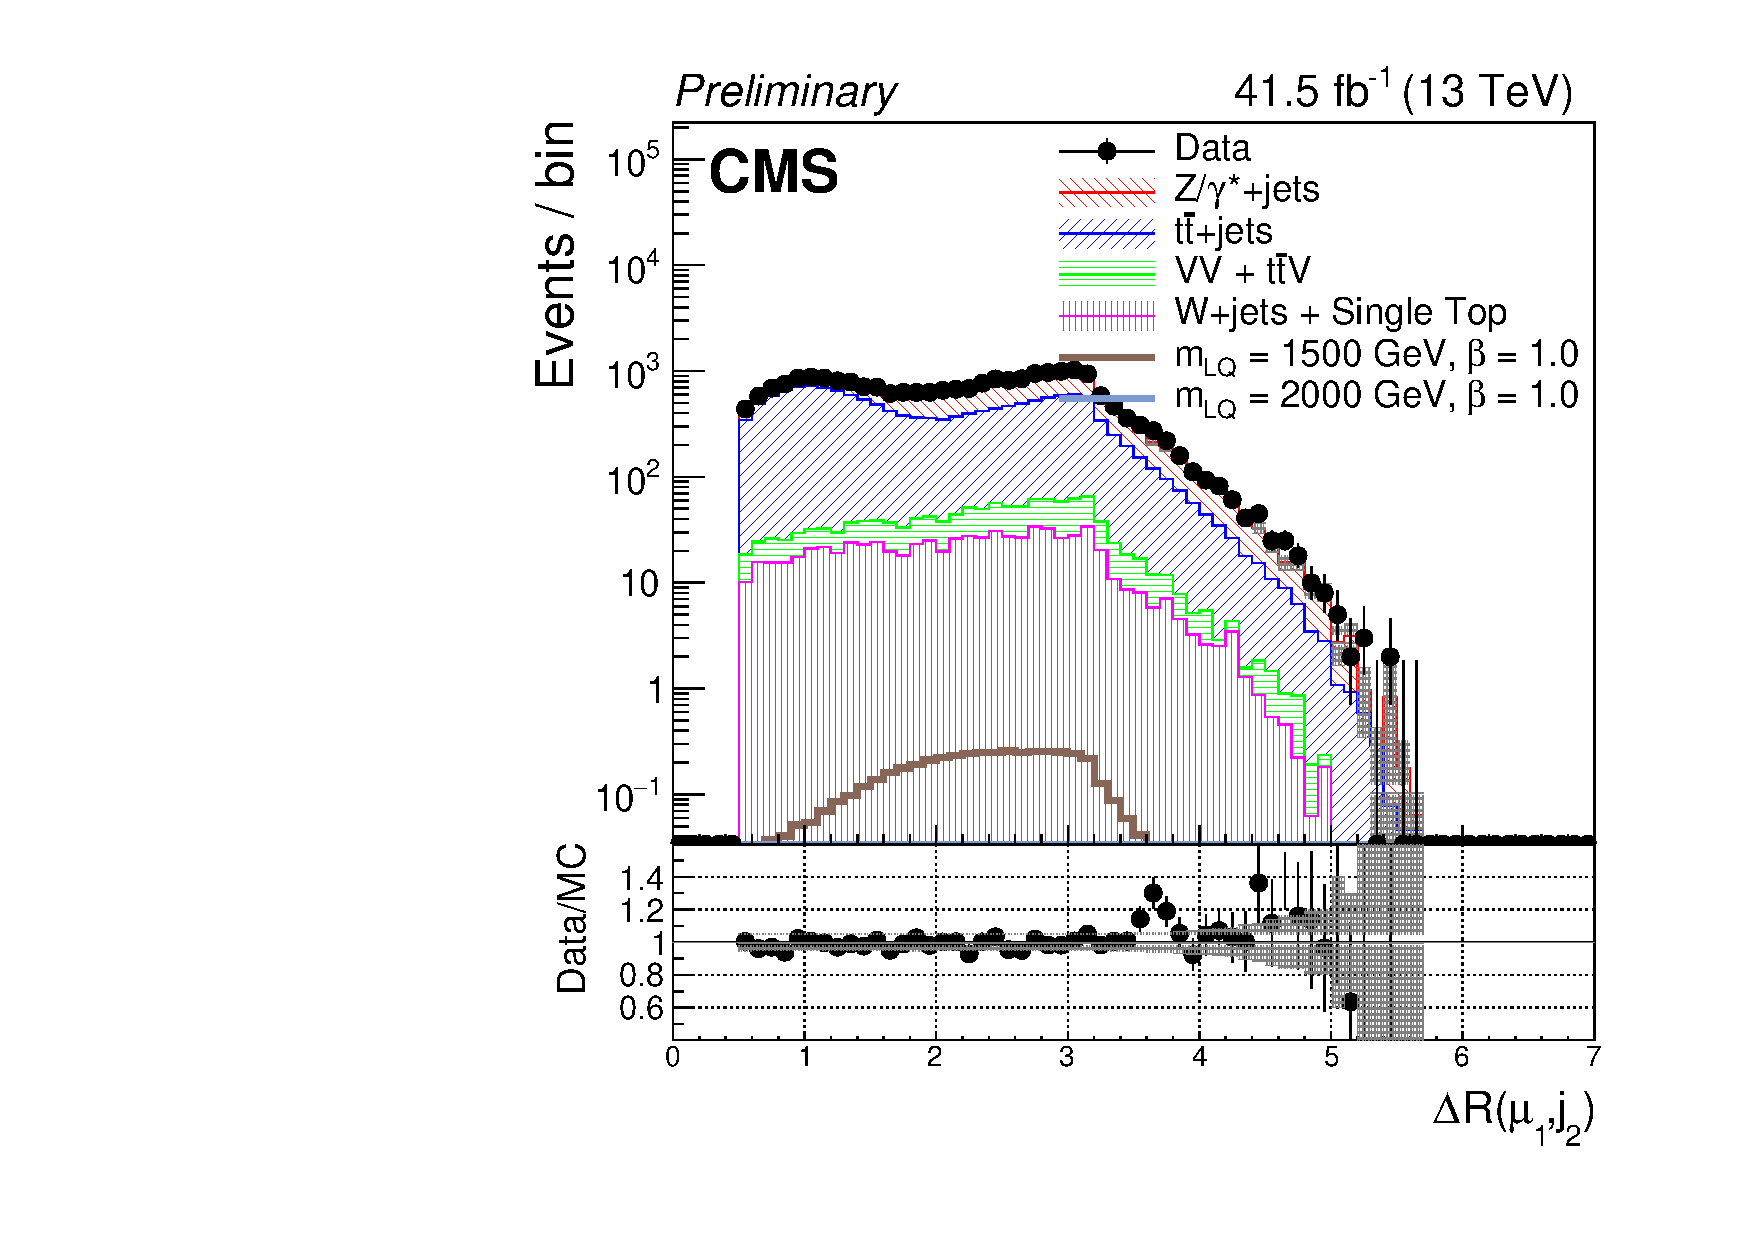
\includegraphics[width=0.32\textwidth]{Images/Analysis/Results_2017_Unblinded/Plots/Preselection/BasicLQ_uujj_DR_muon1jet2_standard.pdf}}
       {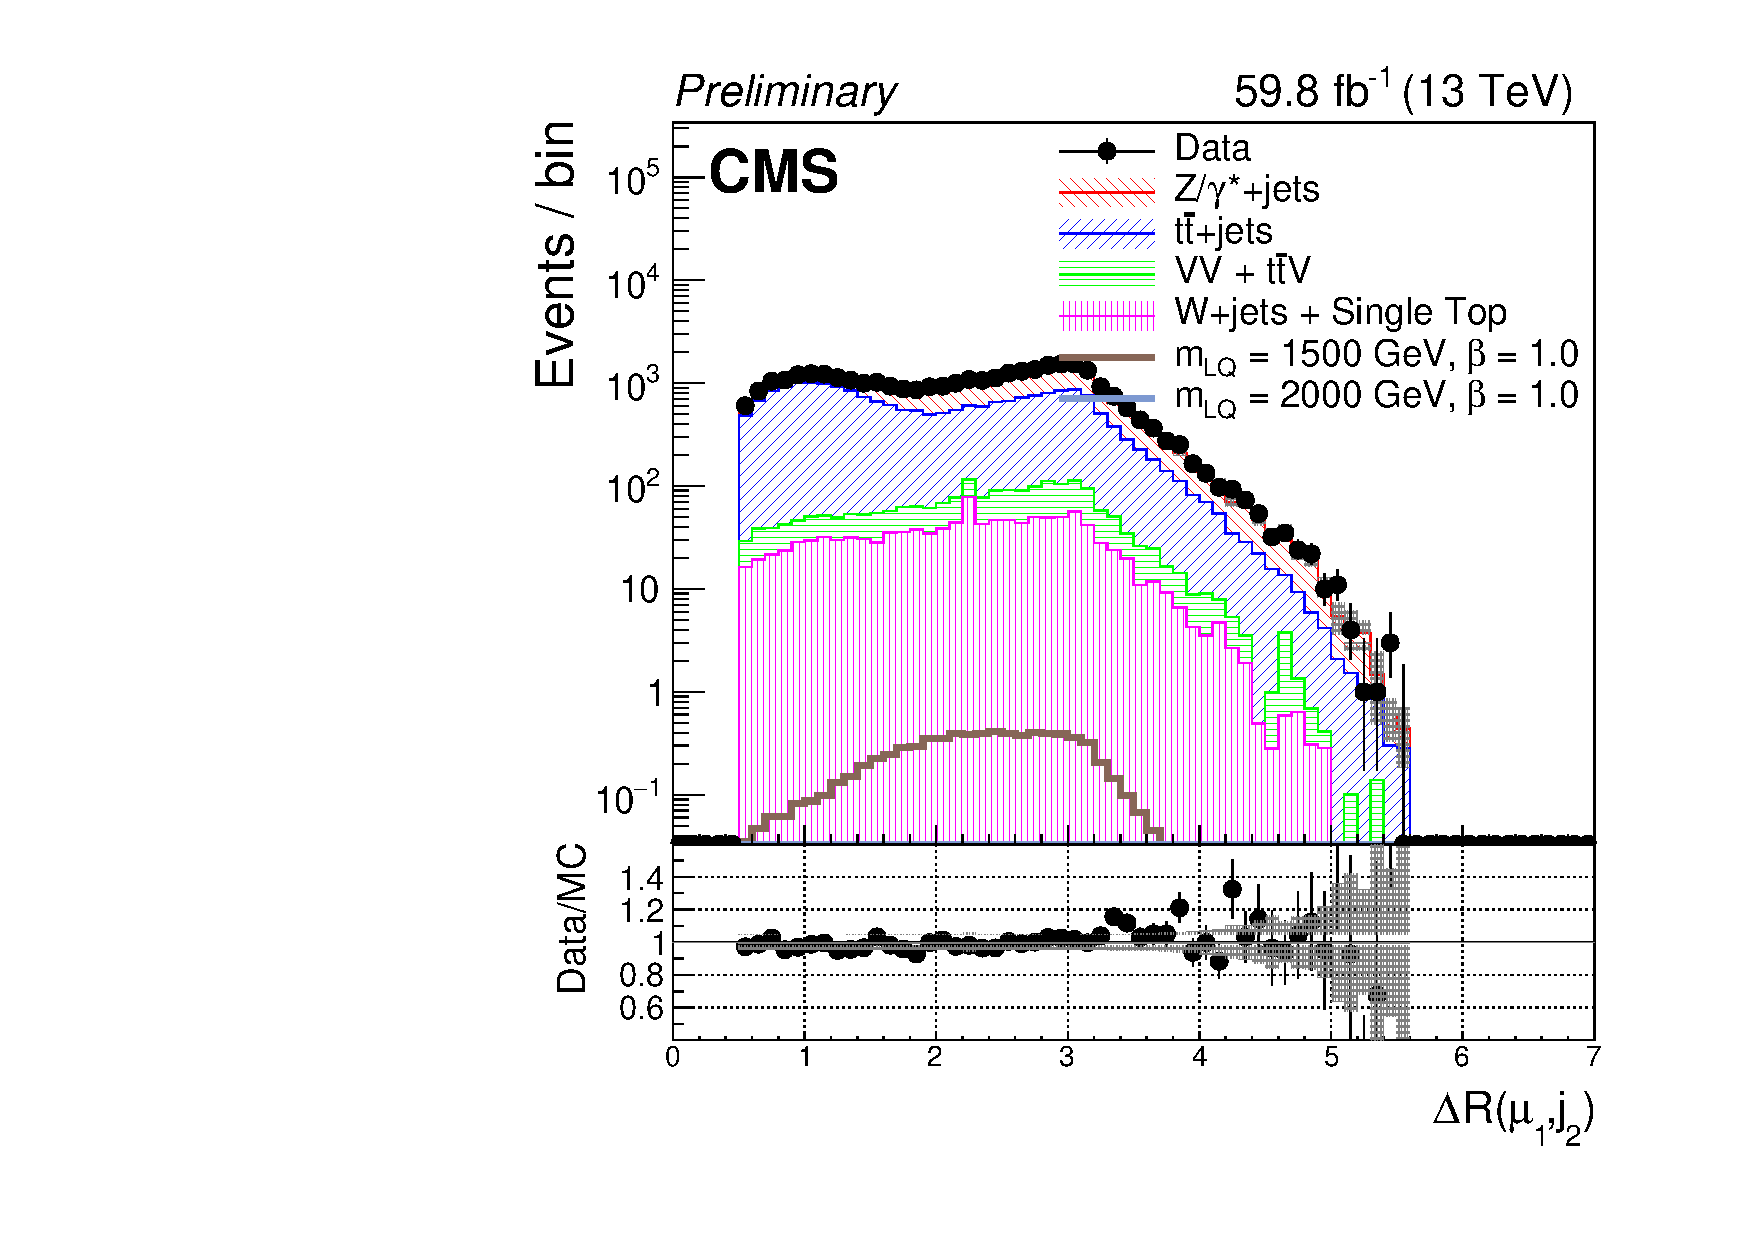
\includegraphics[width=0.32\textwidth]{Images/Analysis/Results_2018_Unblinded/Plots/Preselection/BasicLQ_uujj_DR_muon1jet2_standard.pdf}}
       {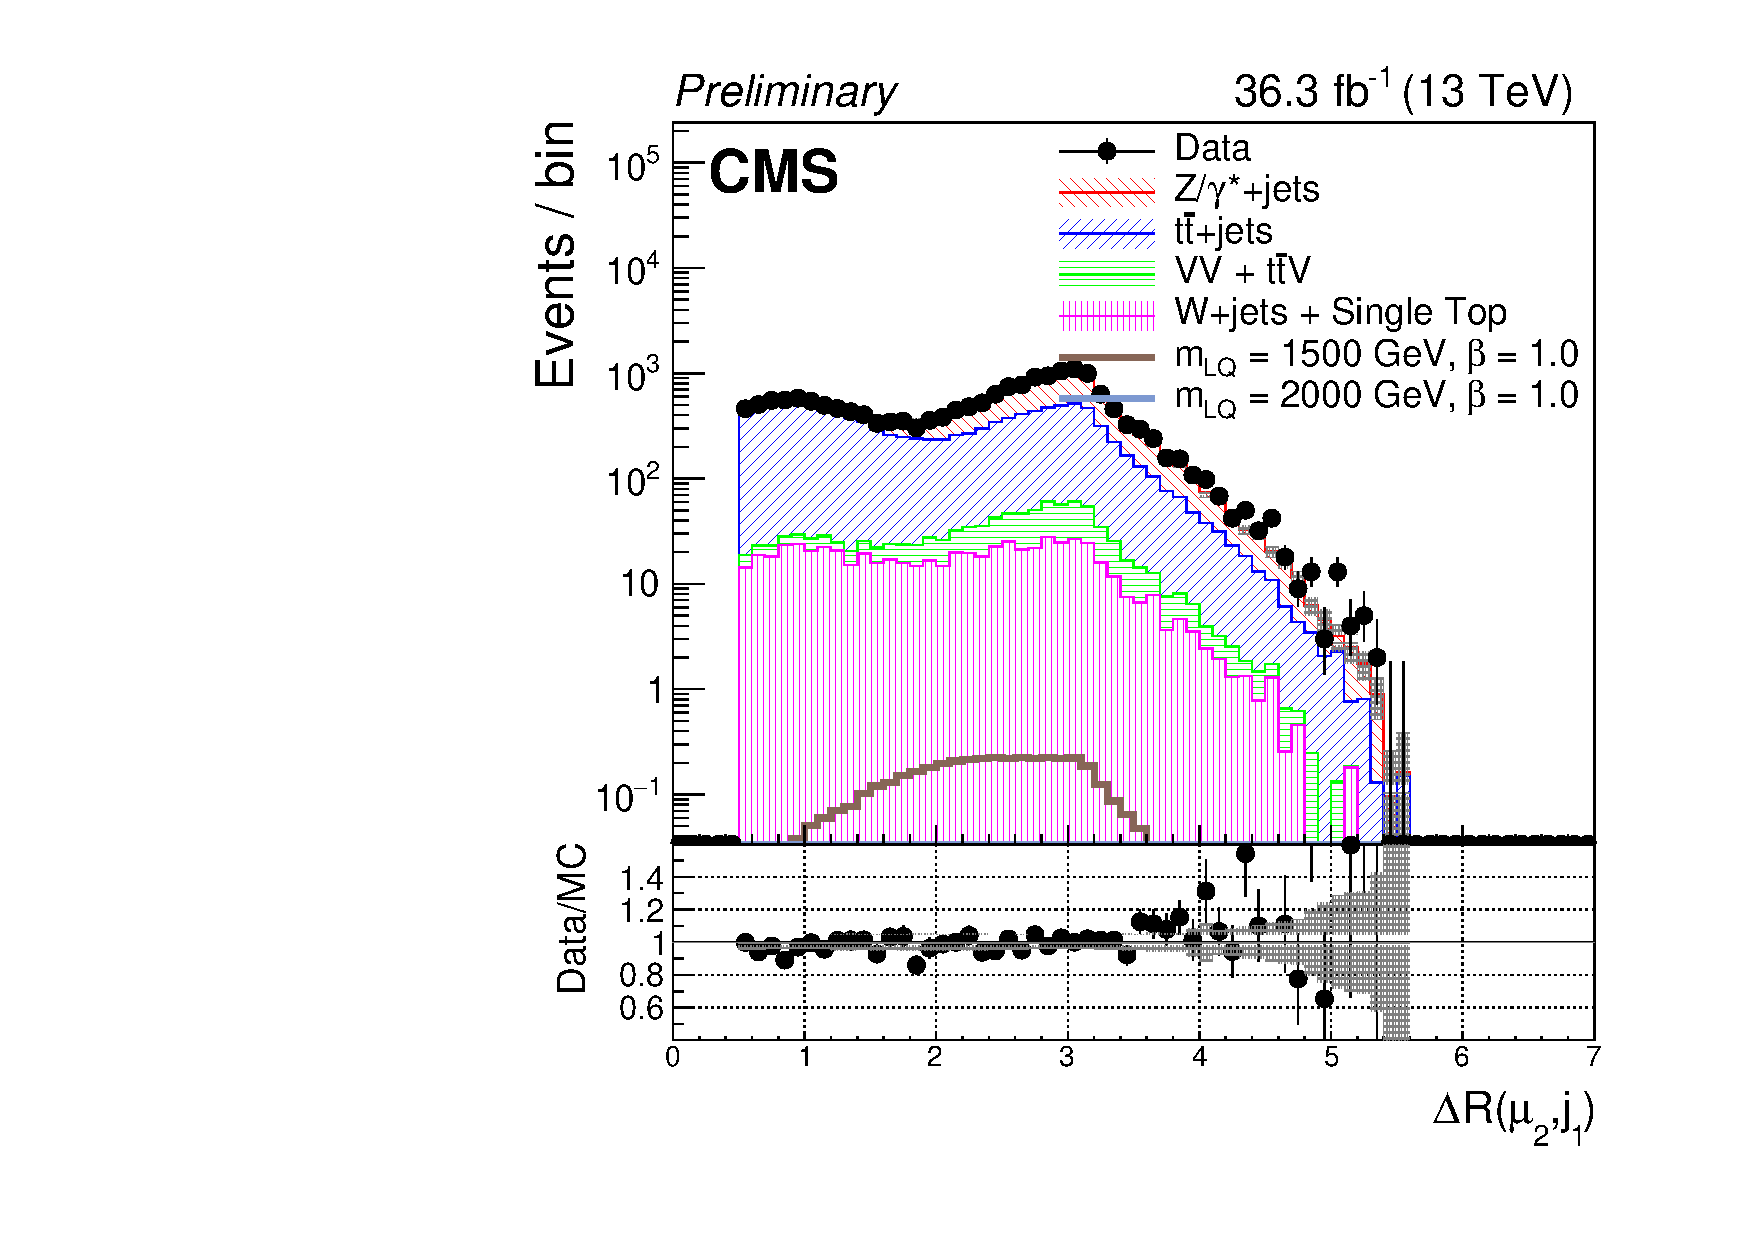
\includegraphics[width=0.32\textwidth]{Images/Analysis/Results_2016_Unblinded/Plots/Preselection/BasicLQ_uujj_DR_muon2jet1_standard.pdf}}
       {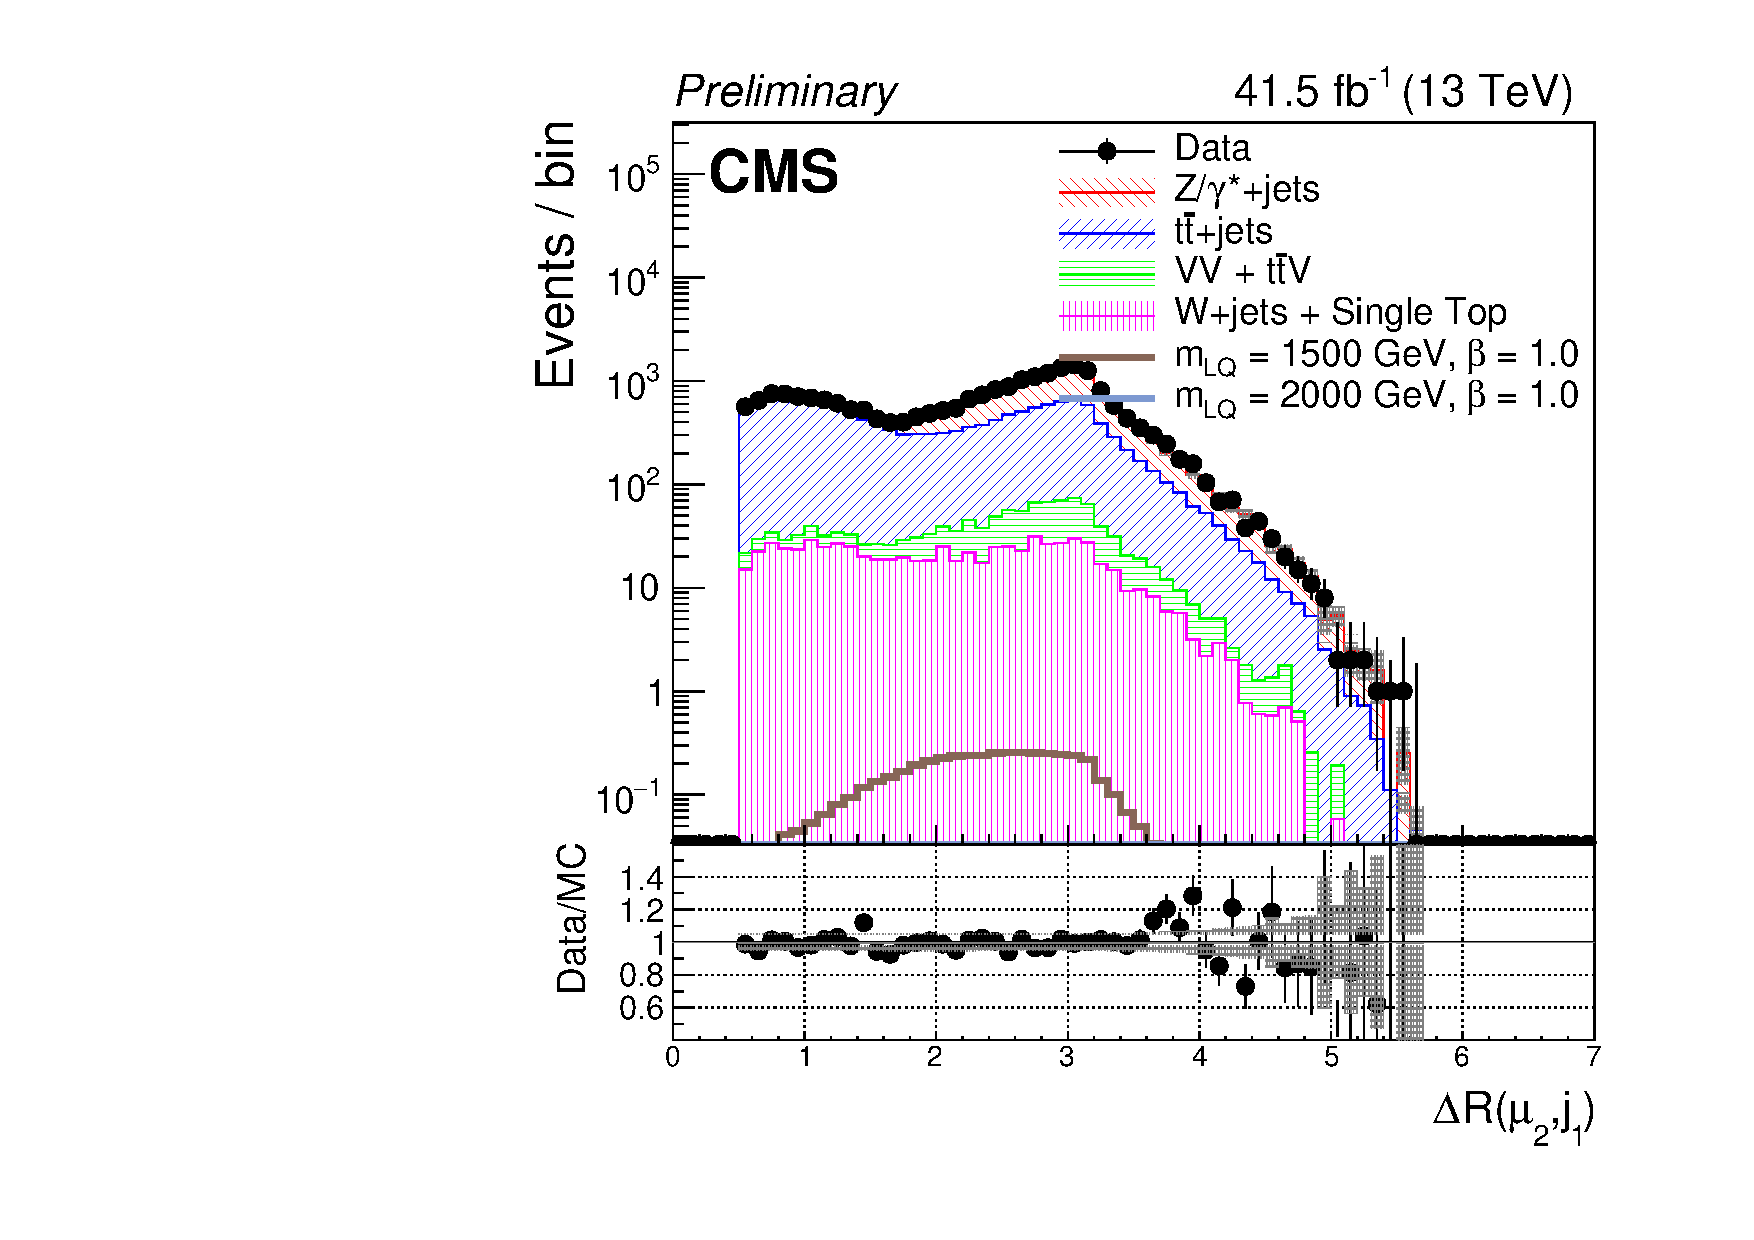
\includegraphics[width=0.32\textwidth]{Images/Analysis/Results_2017_Unblinded/Plots/Preselection/BasicLQ_uujj_DR_muon2jet1_standard.pdf}}
       {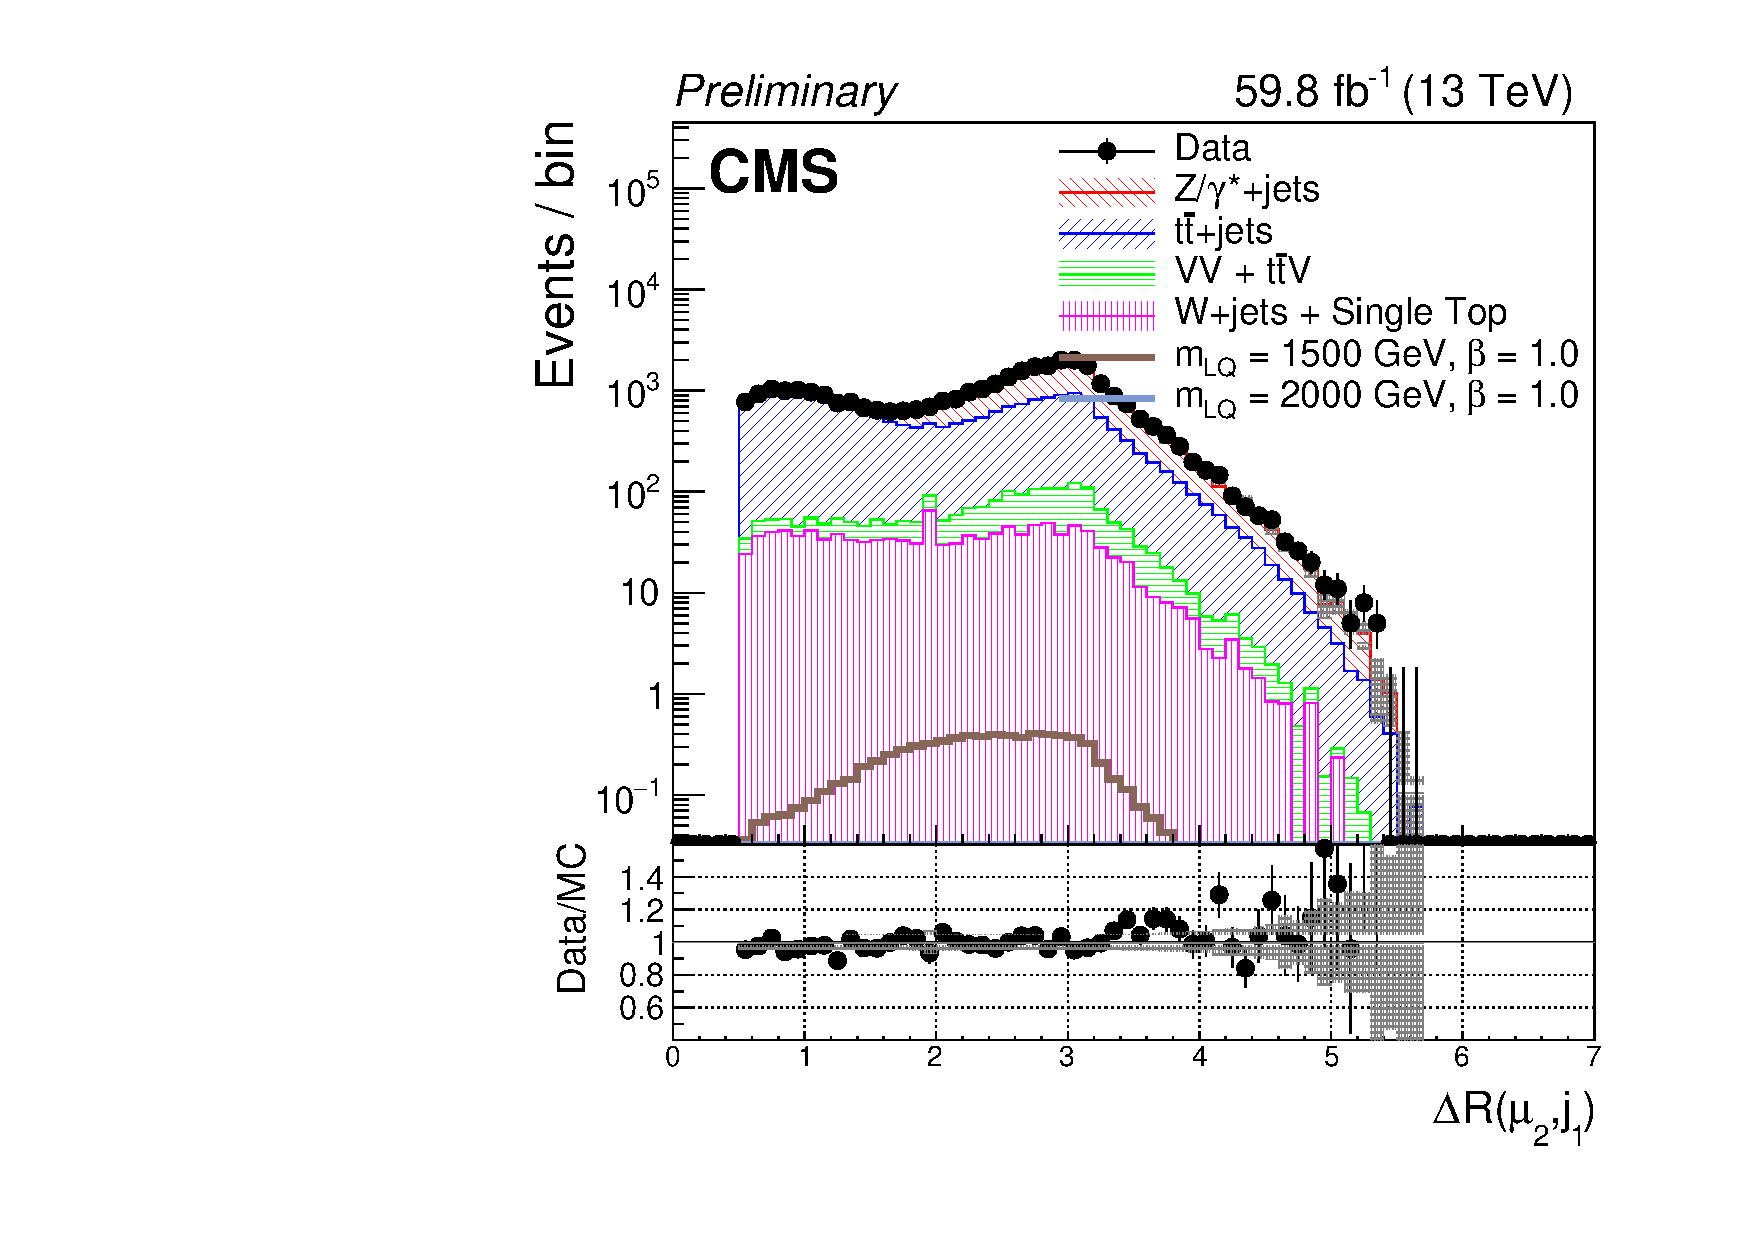
\includegraphics[width=0.32\textwidth]{Images/Analysis/Results_2018_Unblinded/Plots/Preselection/BasicLQ_uujj_DR_muon2jet1_standard.pdf}}
       {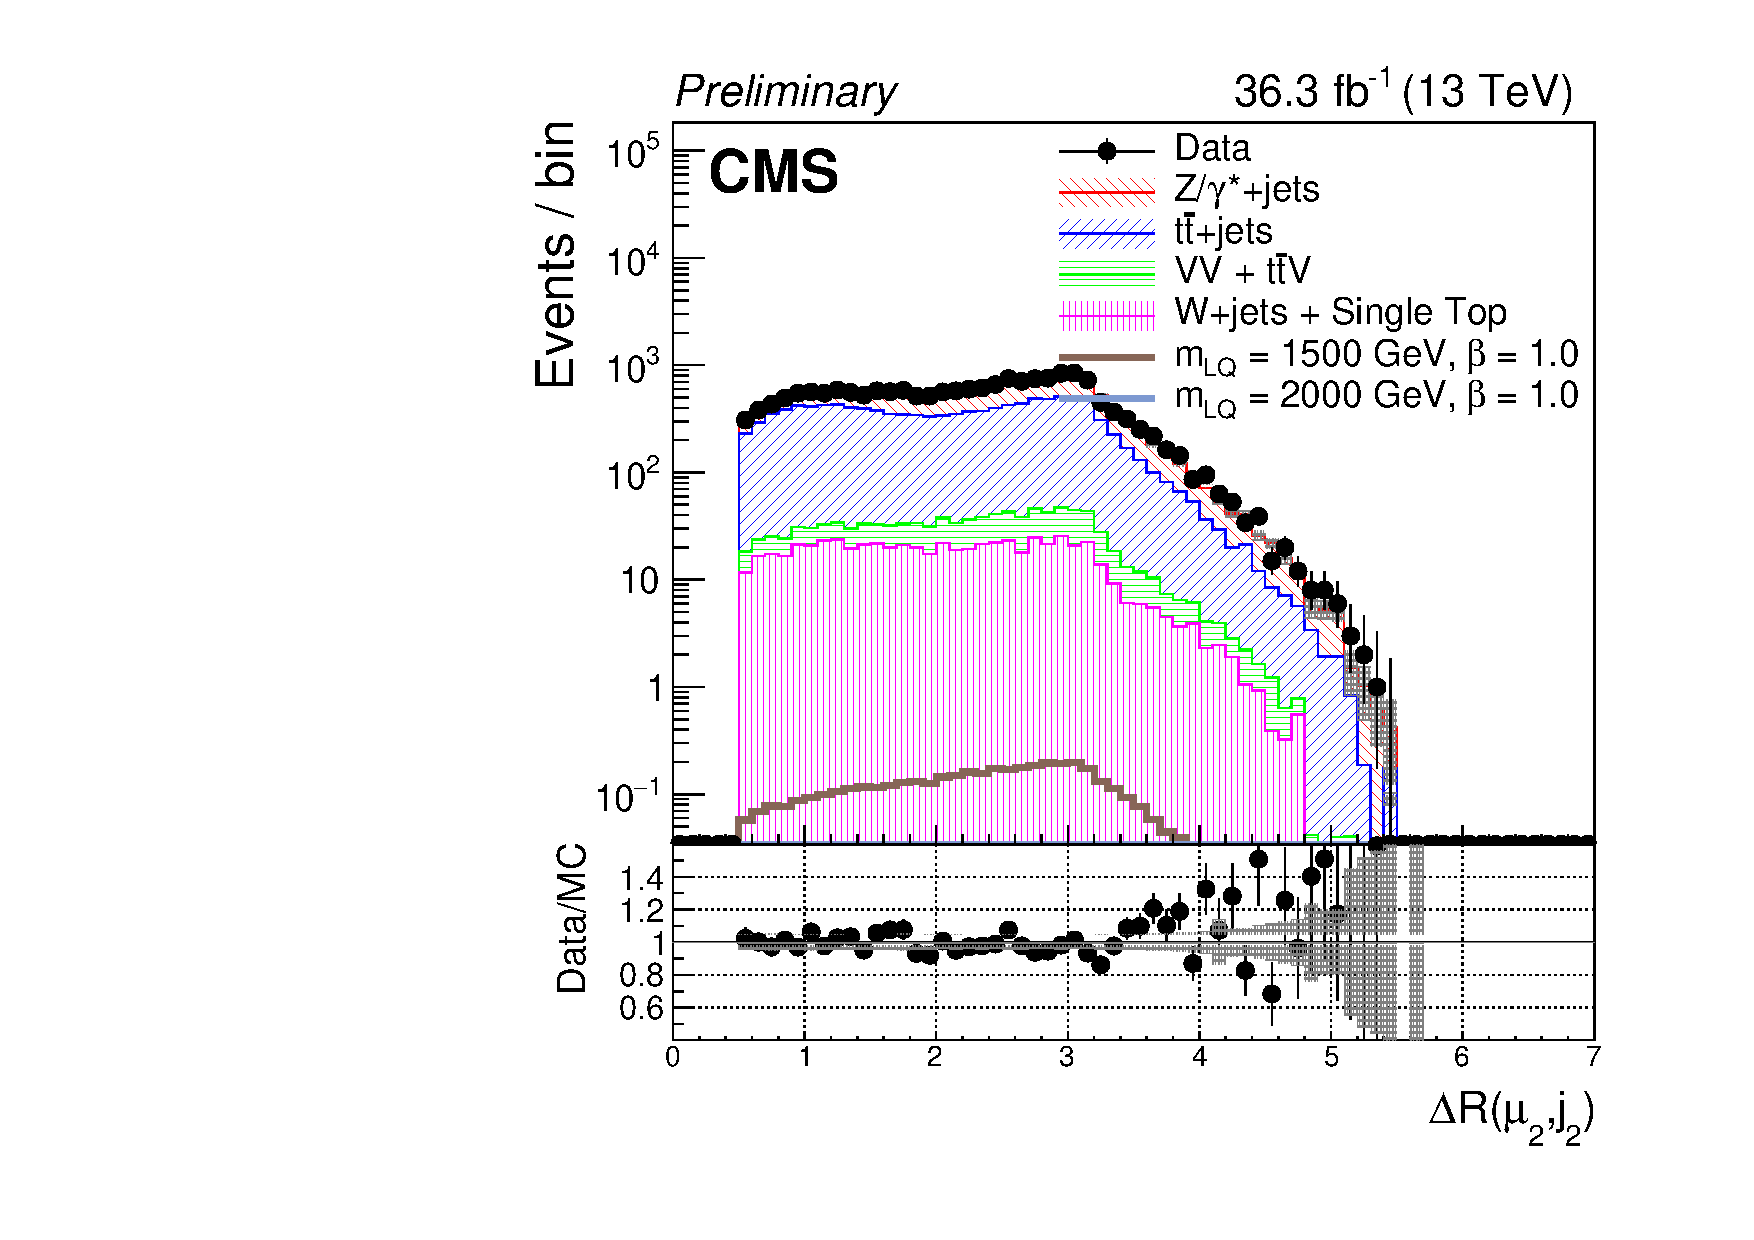
\includegraphics[width=0.32\textwidth]{Images/Analysis/Results_2016_Unblinded/Plots/Preselection/BasicLQ_uujj_DR_muon2jet2_standard.pdf}}
       {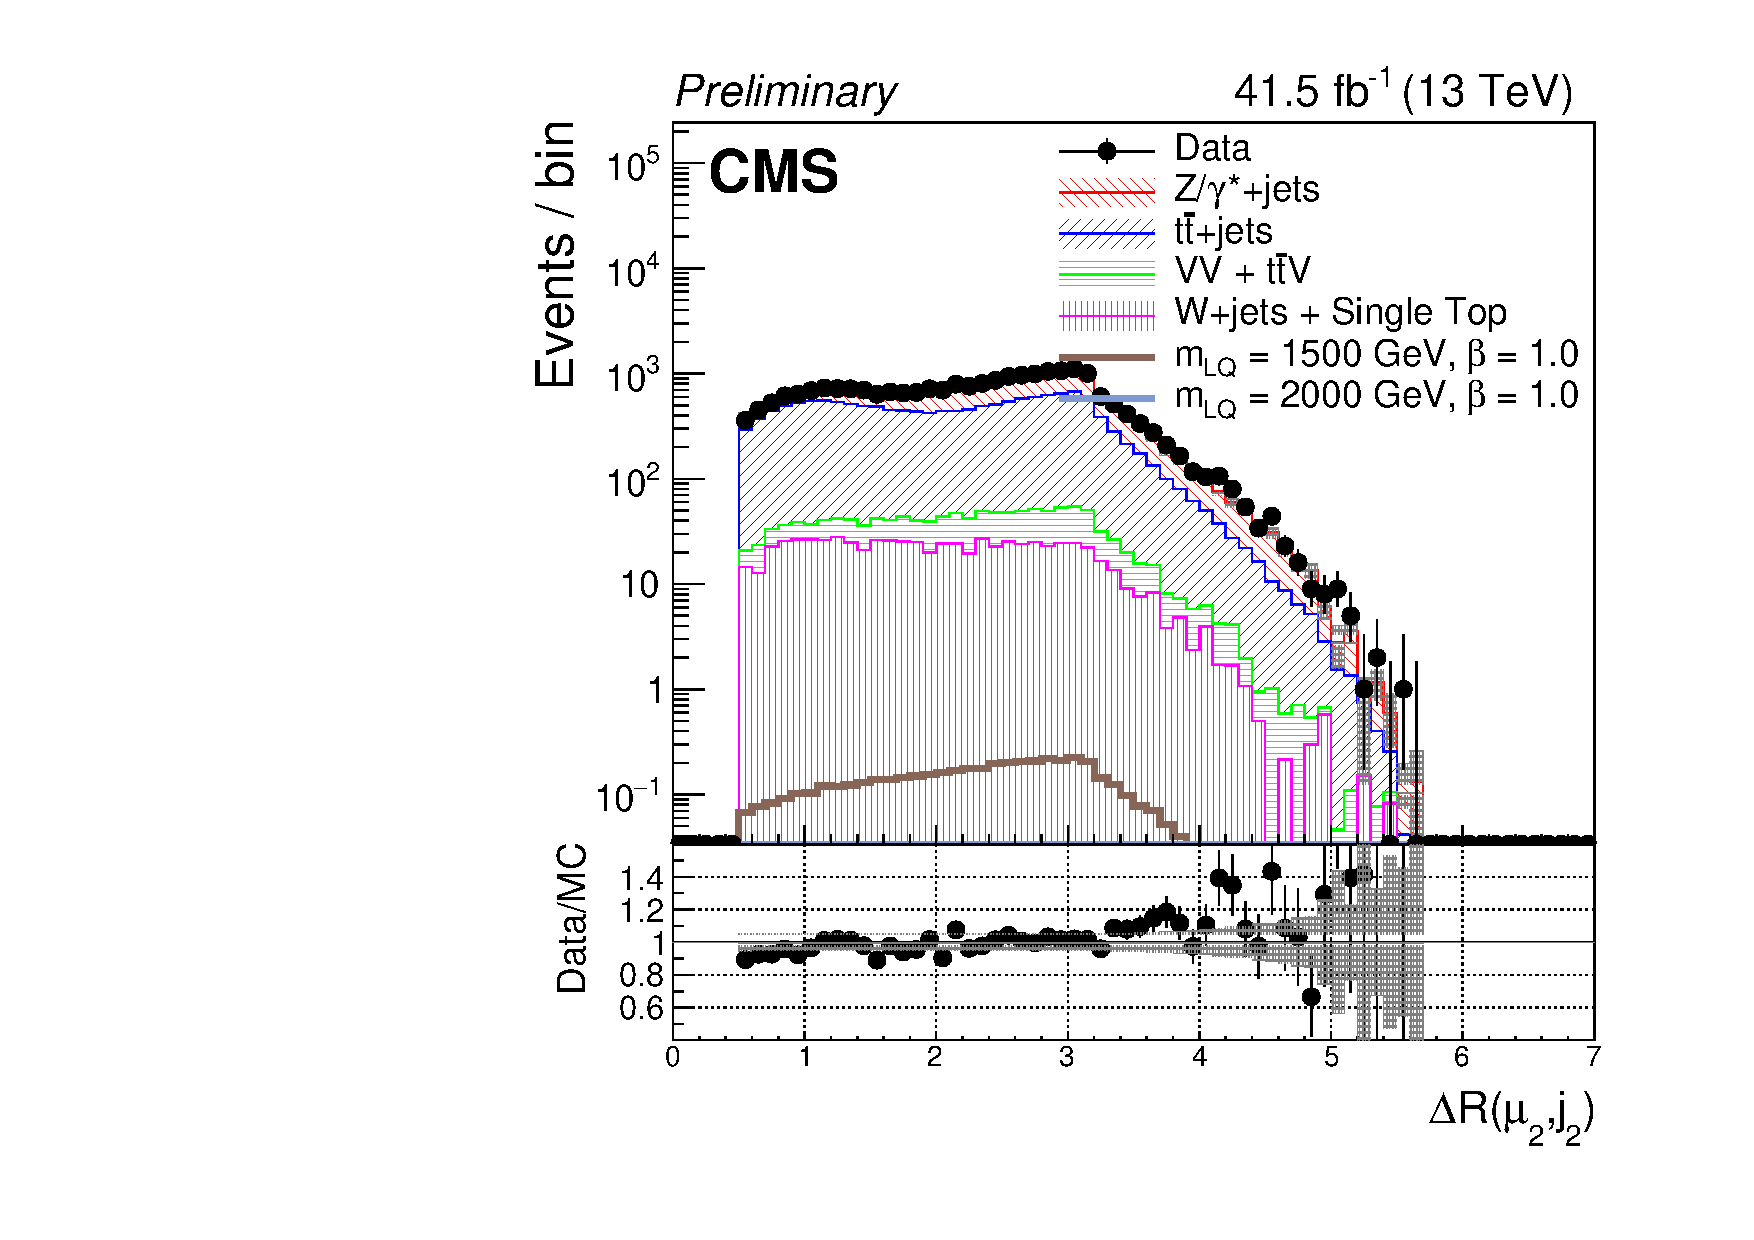
\includegraphics[width=0.32\textwidth]{Images/Analysis/Results_2017_Unblinded/Plots/Preselection/BasicLQ_uujj_DR_muon2jet2_standard.pdf}}
       {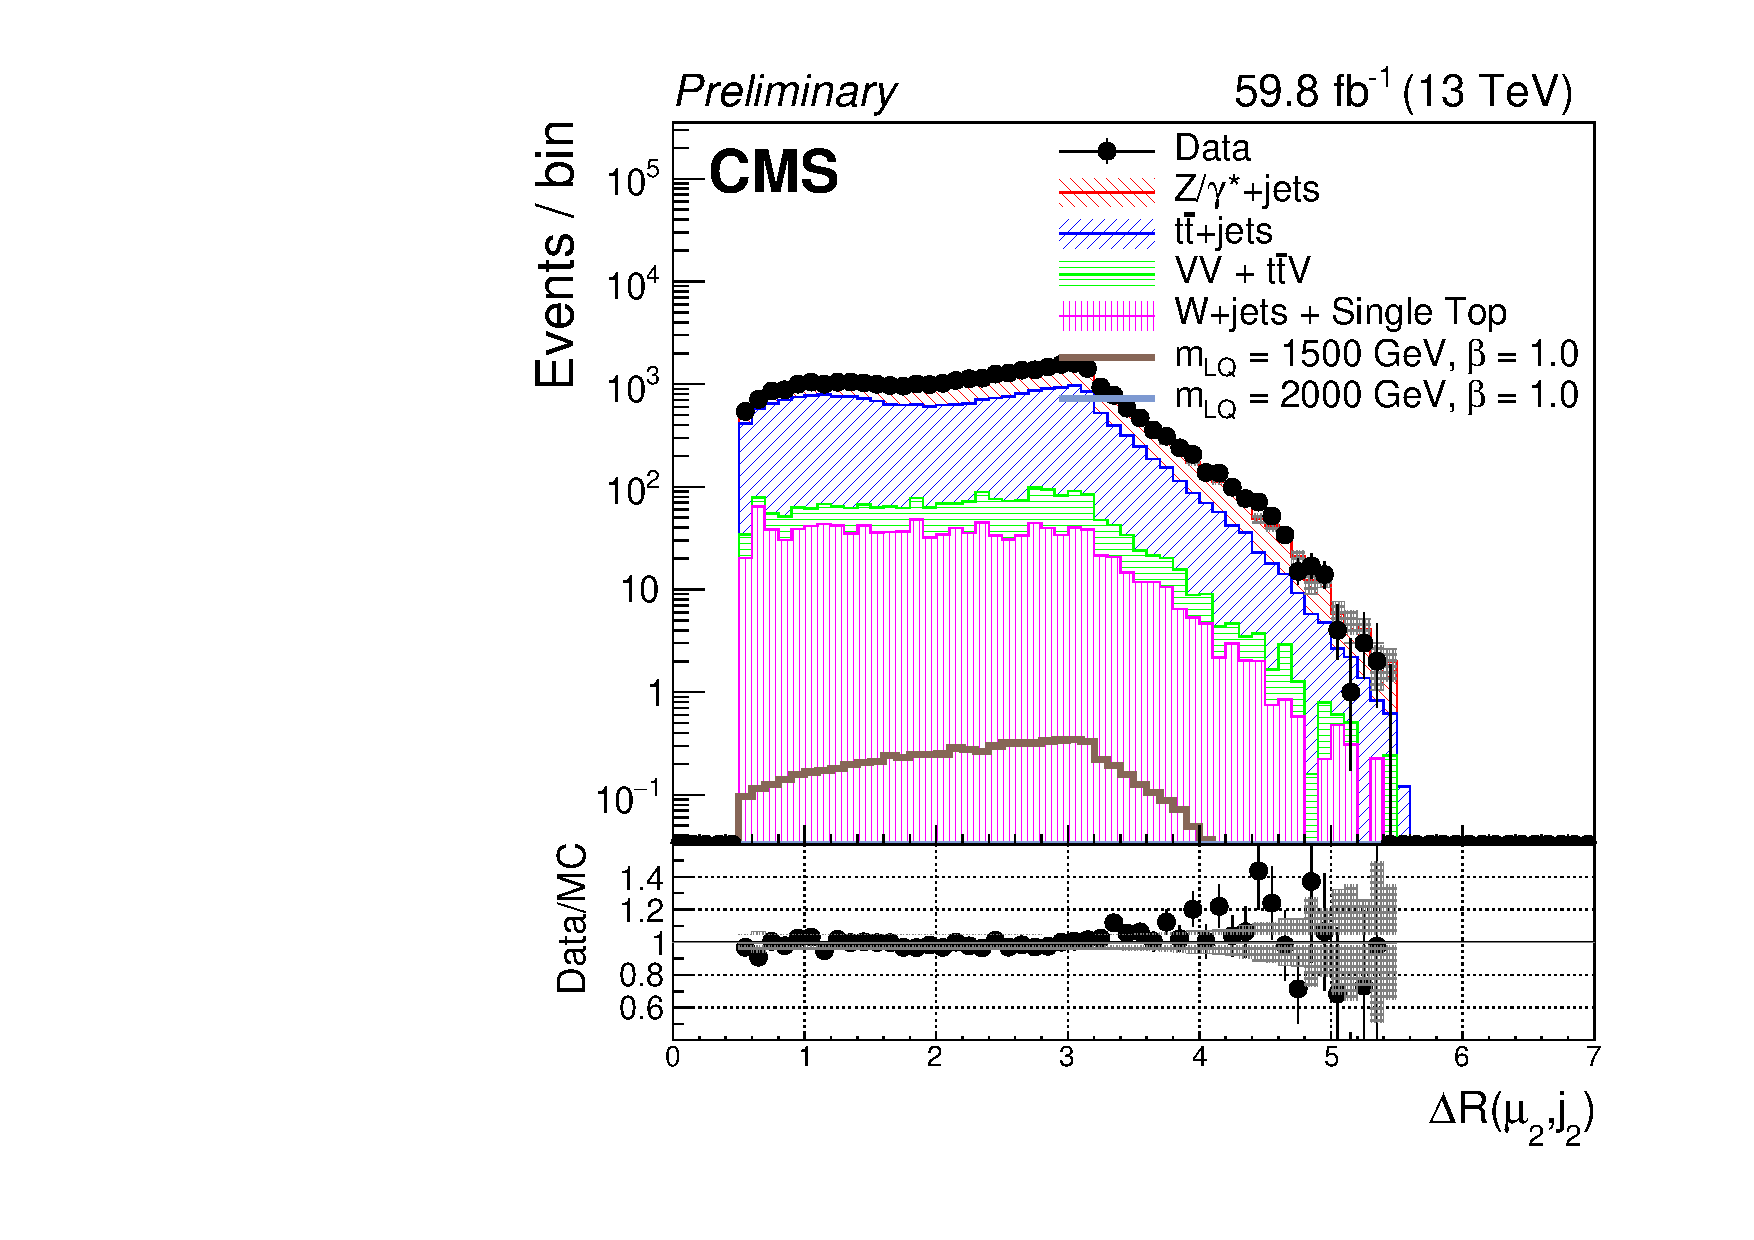
\includegraphics[width=0.32\textwidth]{Images/Analysis/Results_2018_Unblinded/Plots/Preselection/BasicLQ_uujj_DR_muon2jet2_standard.pdf}}
       \caption{A comparison between distributions of observed data and SM expectation at preselection level. Left to right: 2016, 2017, 2018 data. Top to bottom: \DR between muon 1 and jet 1, \DR between muon 1 and jet 2, \DR between muon 2 and jet 1, and \DR between muon 2 and jet 2. Error bars on observed data points represent statistical uncertainties, and systematic uncertainties on SM expectation are shown by gray hashing.}
       \label{figapp:preseldr}
\end{figure}

\begin{figure}[H]
       \centering
       {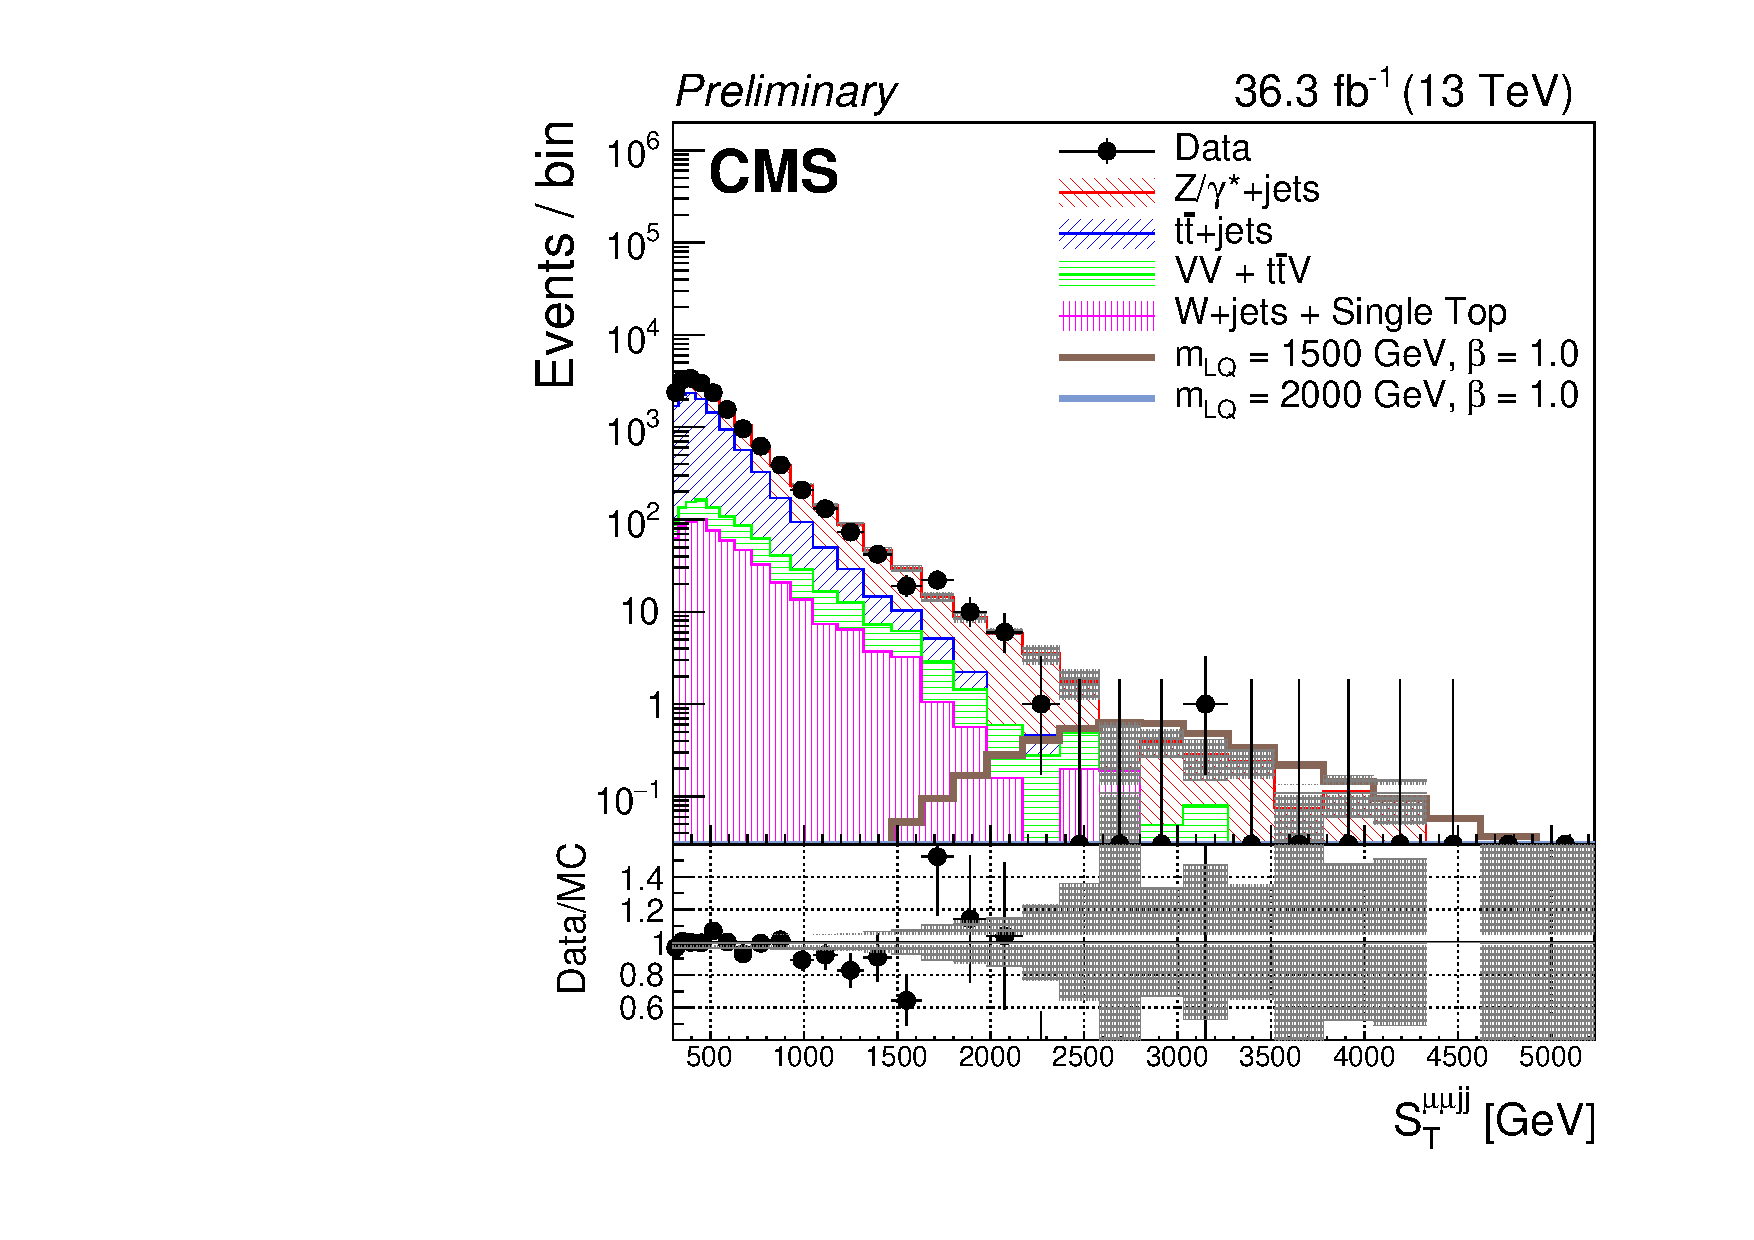
\includegraphics[width=.32\textwidth]{Images/Analysis/Results_2016_Unblinded/Plots/Preselection/BasicLQ_uujj_St_uujj_standard.pdf}}
       {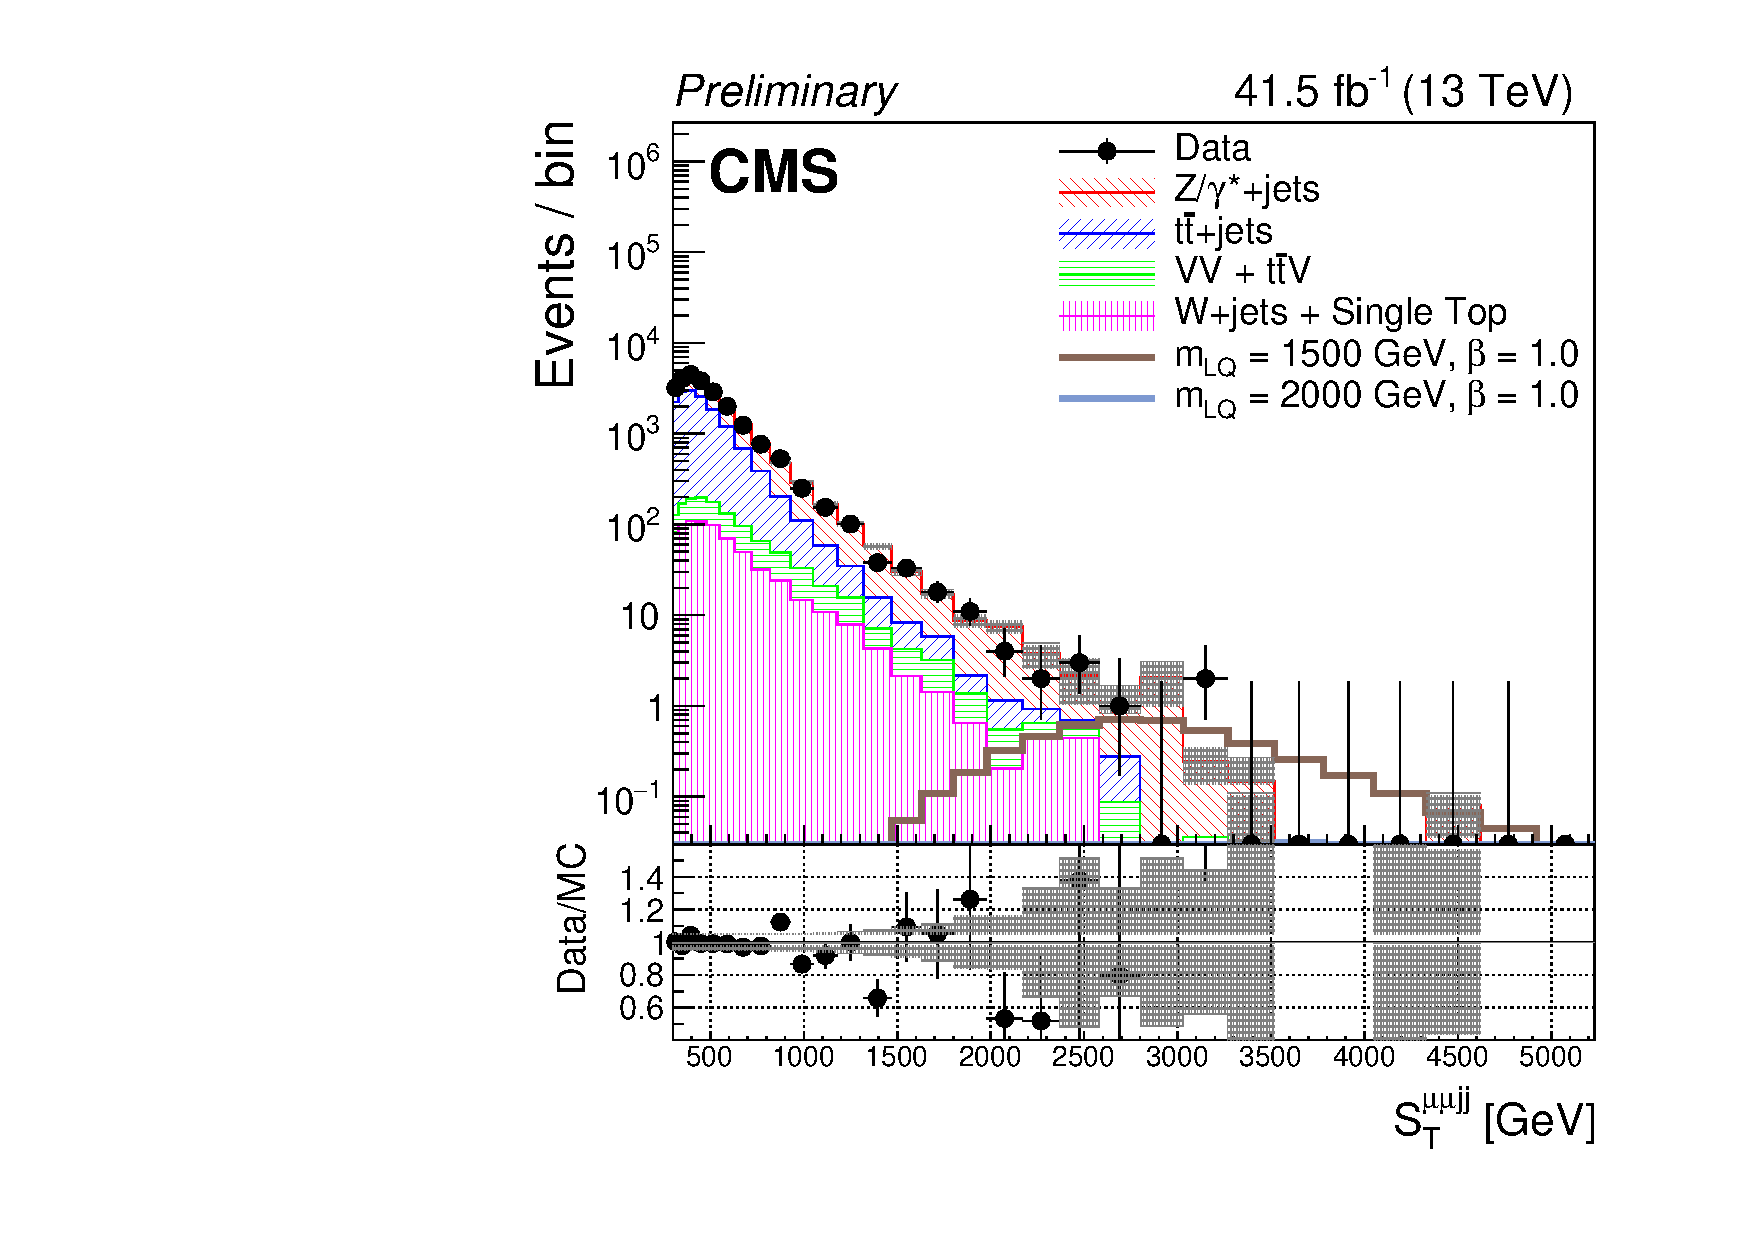
\includegraphics[width=.32\textwidth]{Images/Analysis/Results_2017_Unblinded/Plots/Preselection/BasicLQ_uujj_St_uujj_standard.pdf}}
       {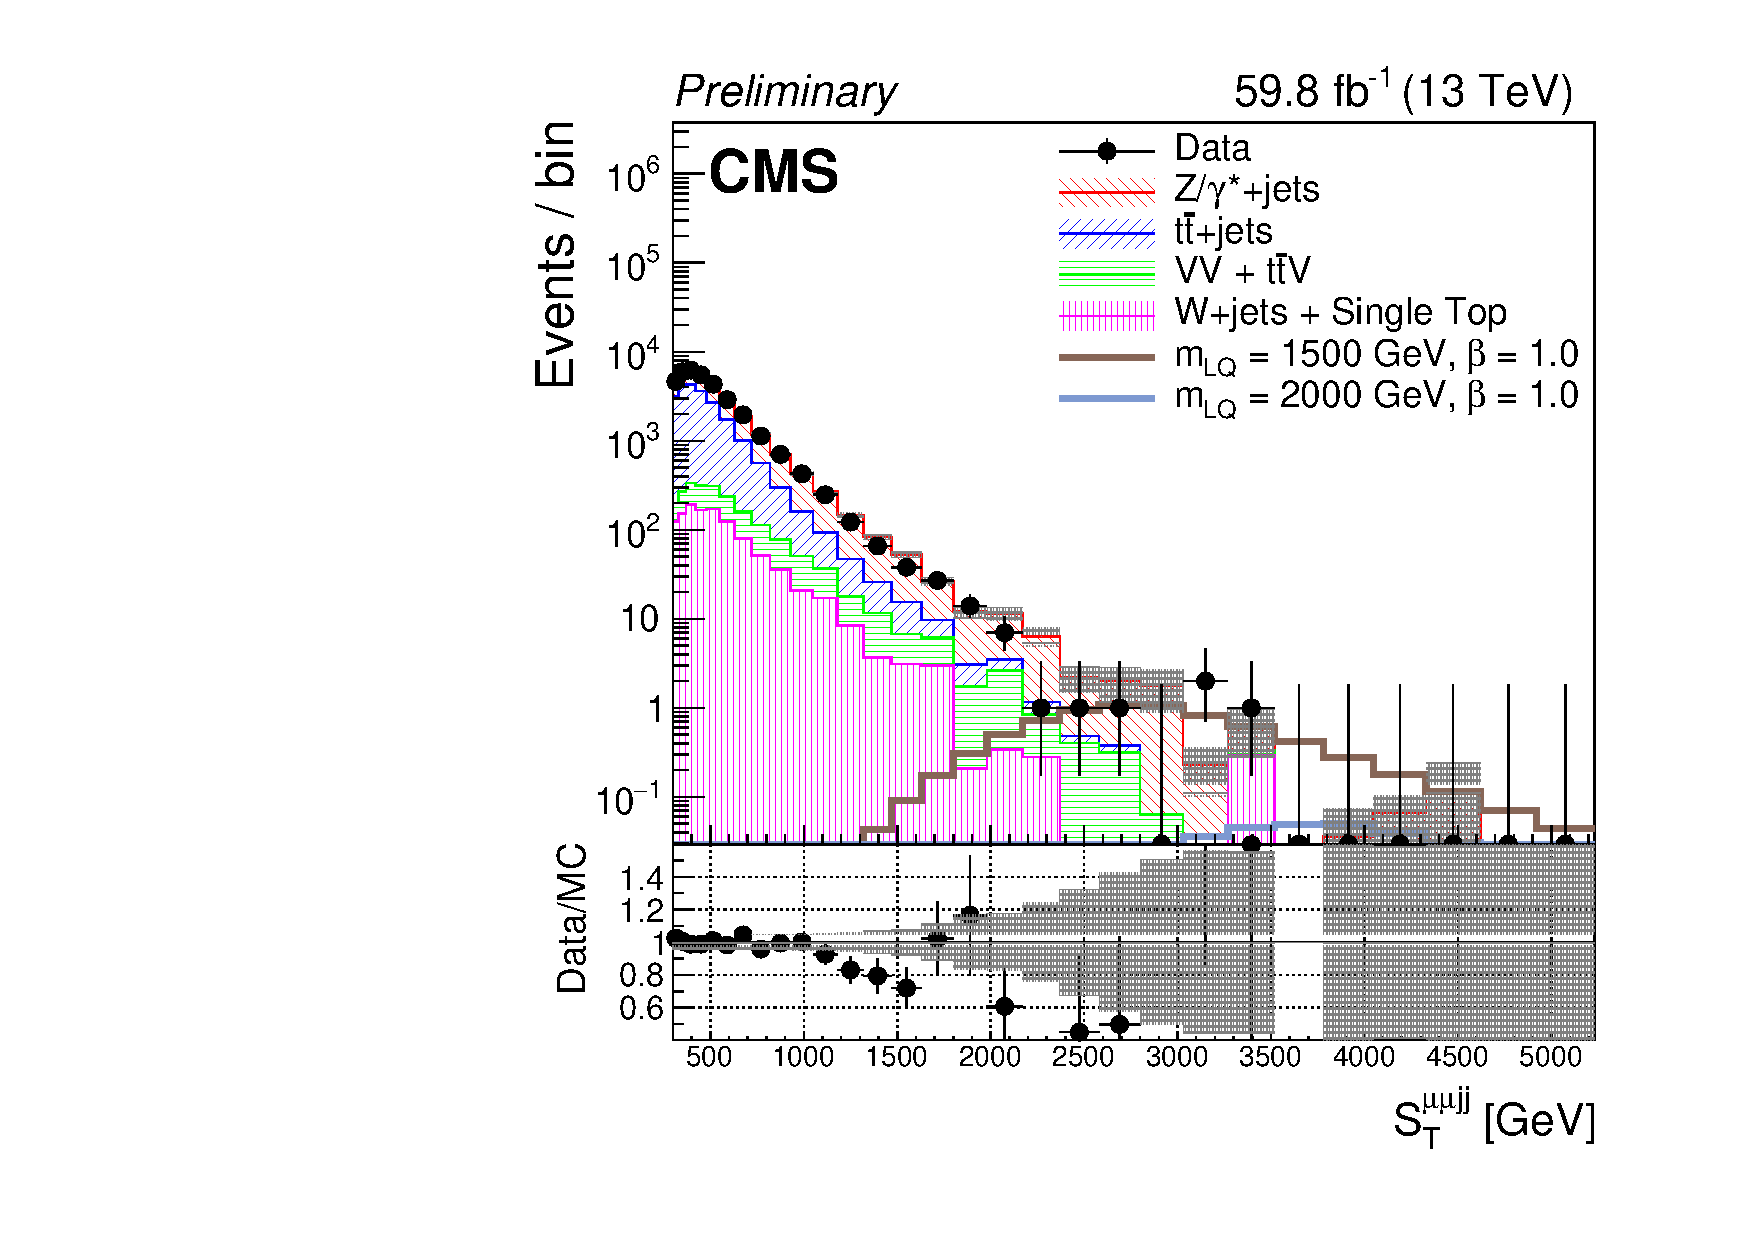
\includegraphics[width=.32\textwidth]{Images/Analysis/Results_2018_Unblinded/Plots/Preselection/BasicLQ_uujj_St_uujj_standard.pdf}}
       {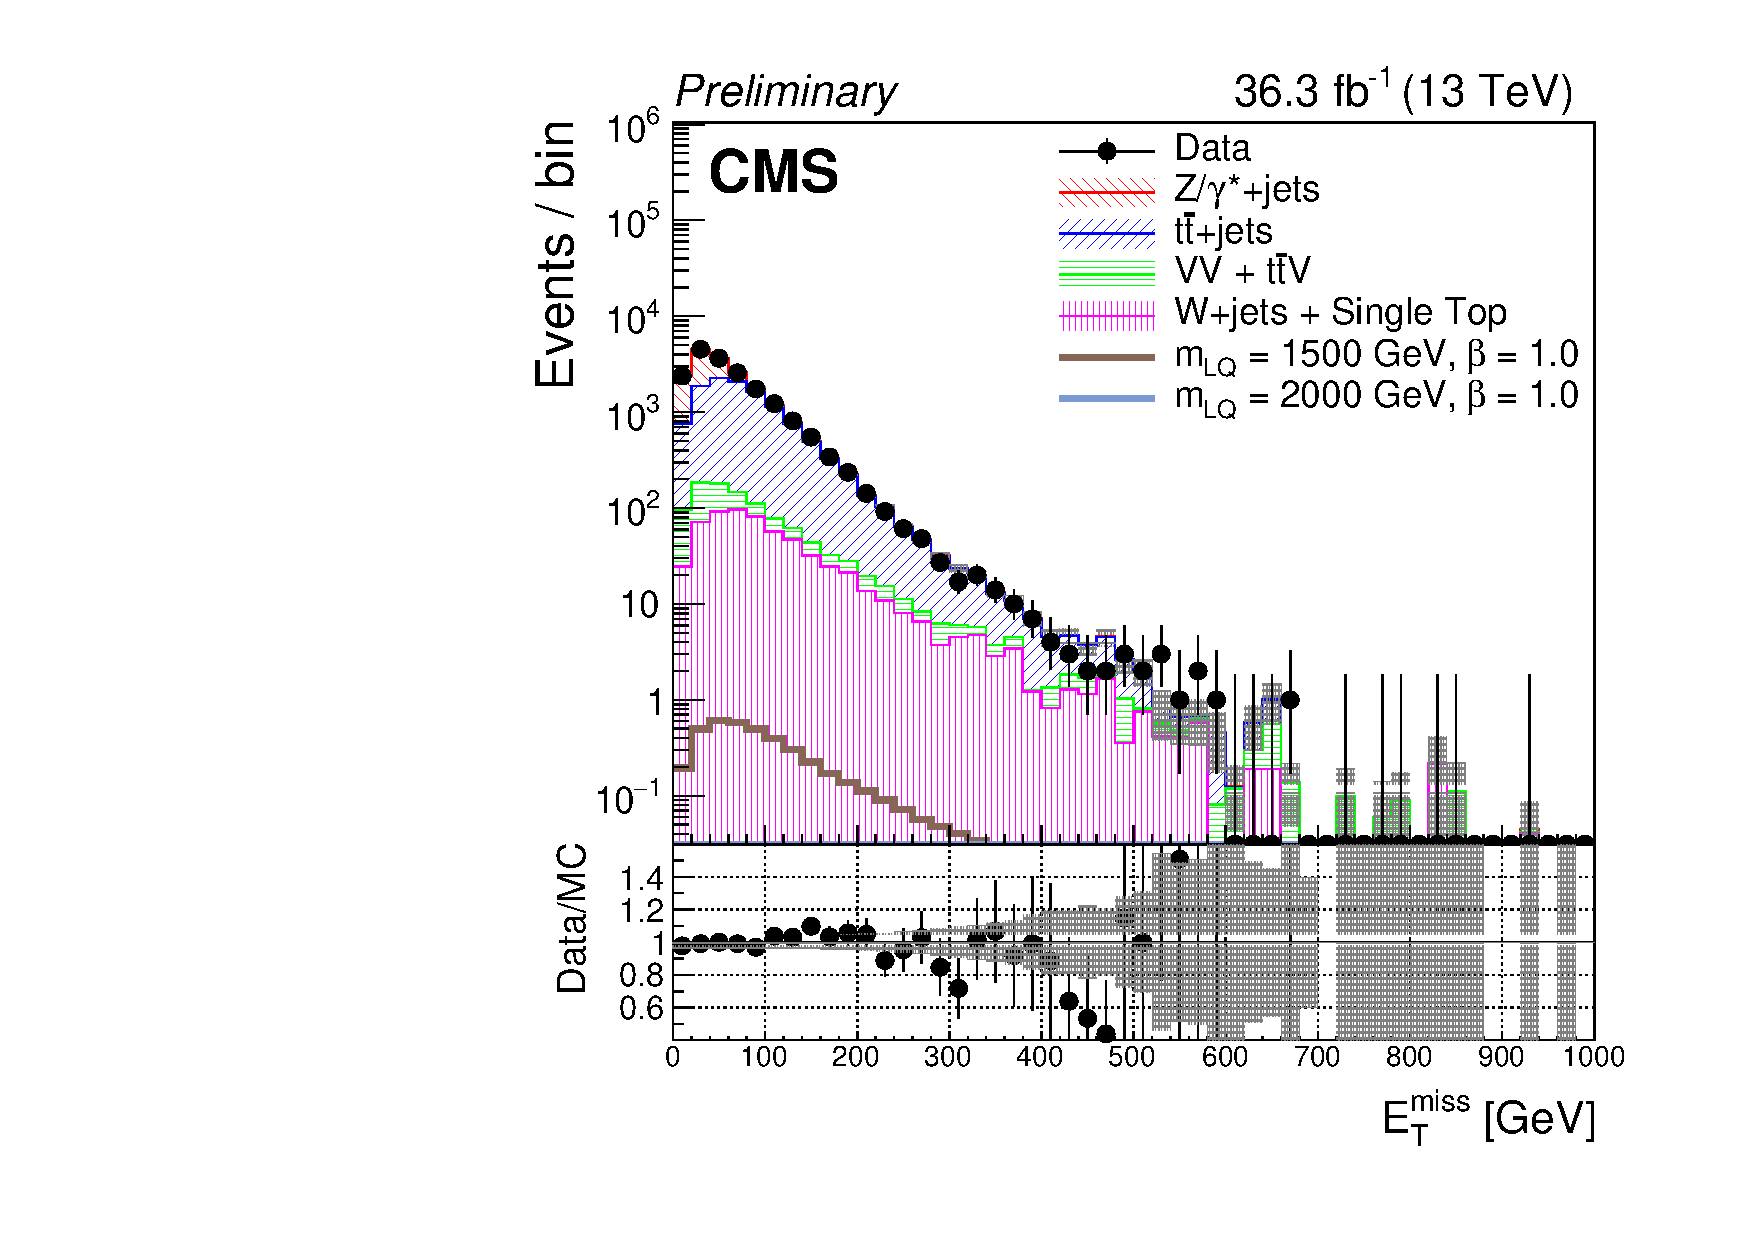
\includegraphics[width=.32\textwidth]{Images/Analysis/Results_2016_Unblinded/Plots/Preselection/BasicLQ_uujj_Pt_miss_standard.pdf}}
       {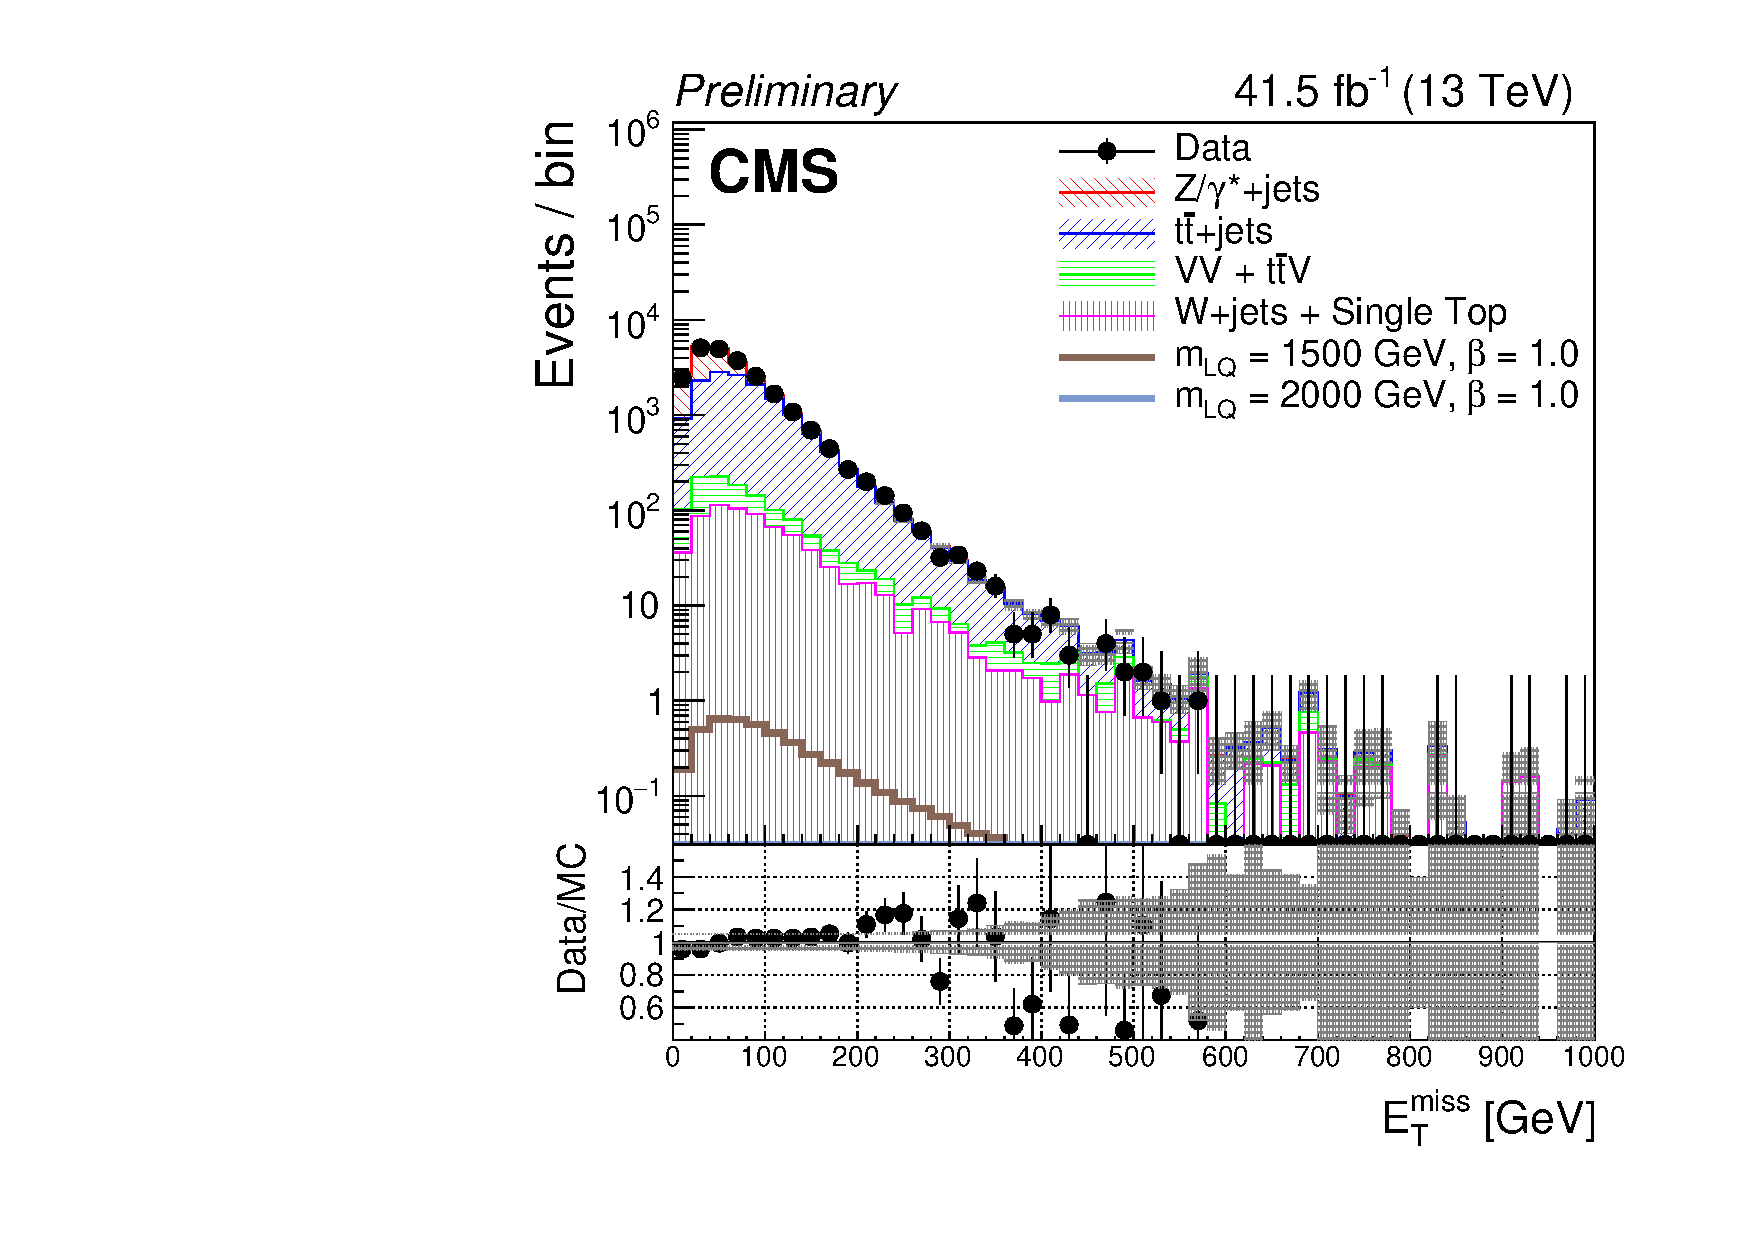
\includegraphics[width=.32\textwidth]{Images/Analysis/Results_2017_Unblinded/Plots/Preselection/BasicLQ_uujj_Pt_miss_standard.pdf}}
       {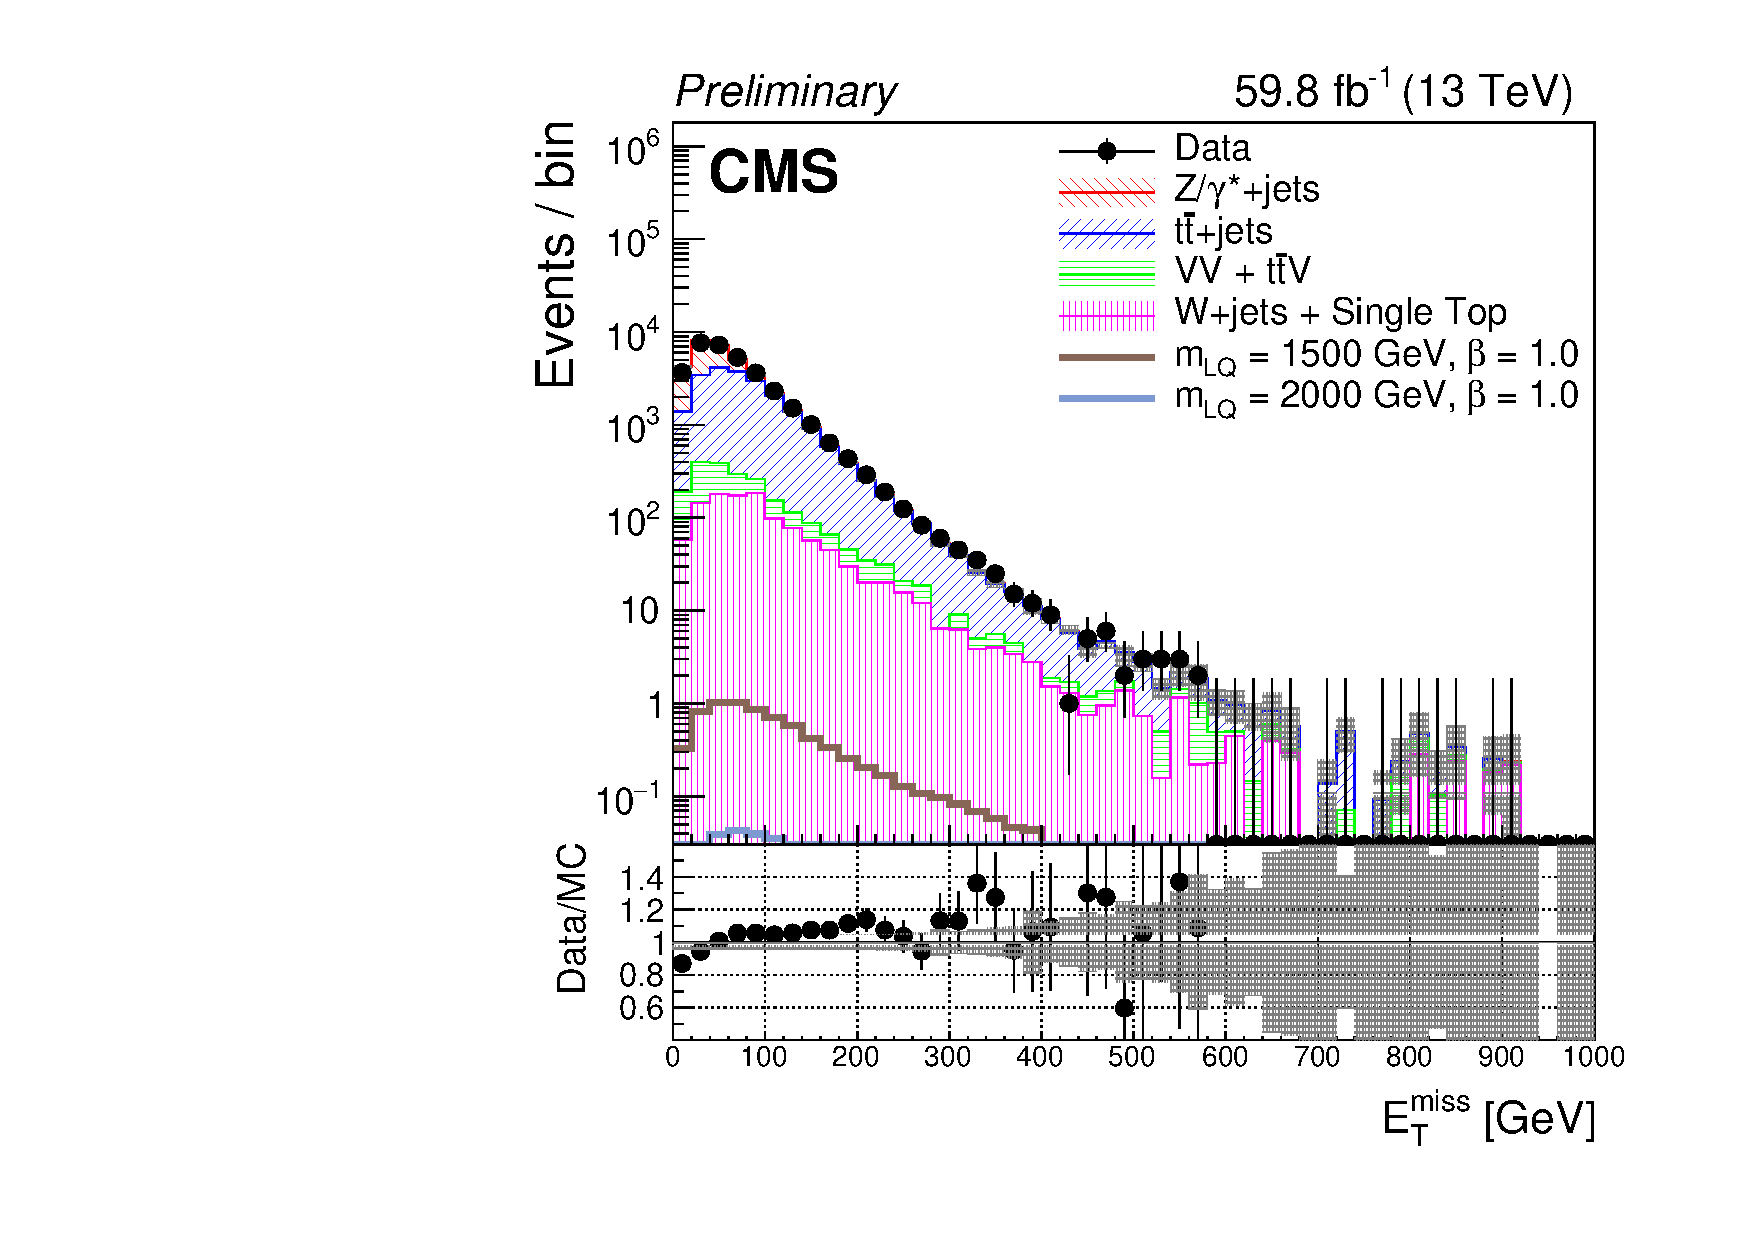
\includegraphics[width=.32\textwidth]{Images/Analysis/Results_2018_Unblinded/Plots/Preselection/BasicLQ_uujj_Pt_miss_standard.pdf}}
       {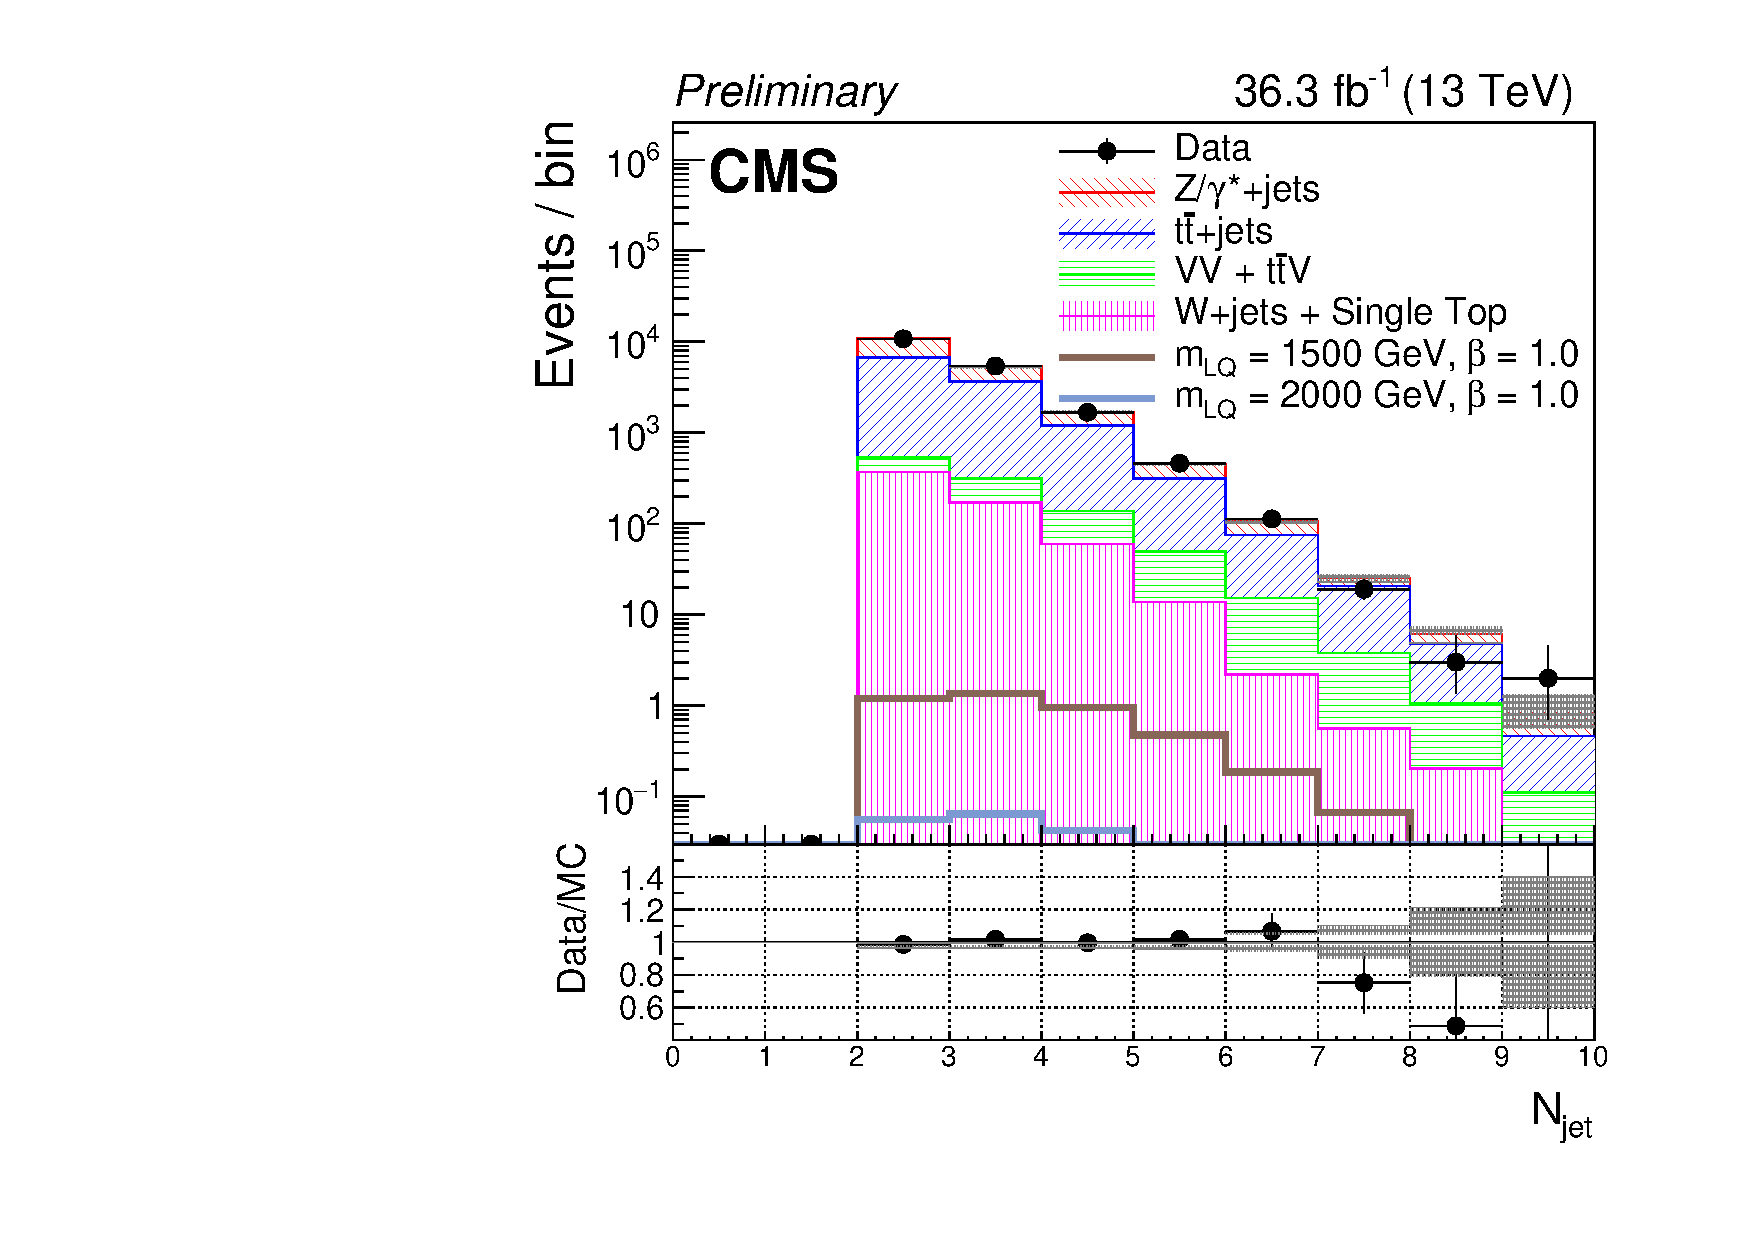
\includegraphics[width=.32\textwidth]{Images/Analysis/Results_2016_Unblinded/Plots/Preselection/BasicLQ_uujj_JetCount_standard.pdf}}
       {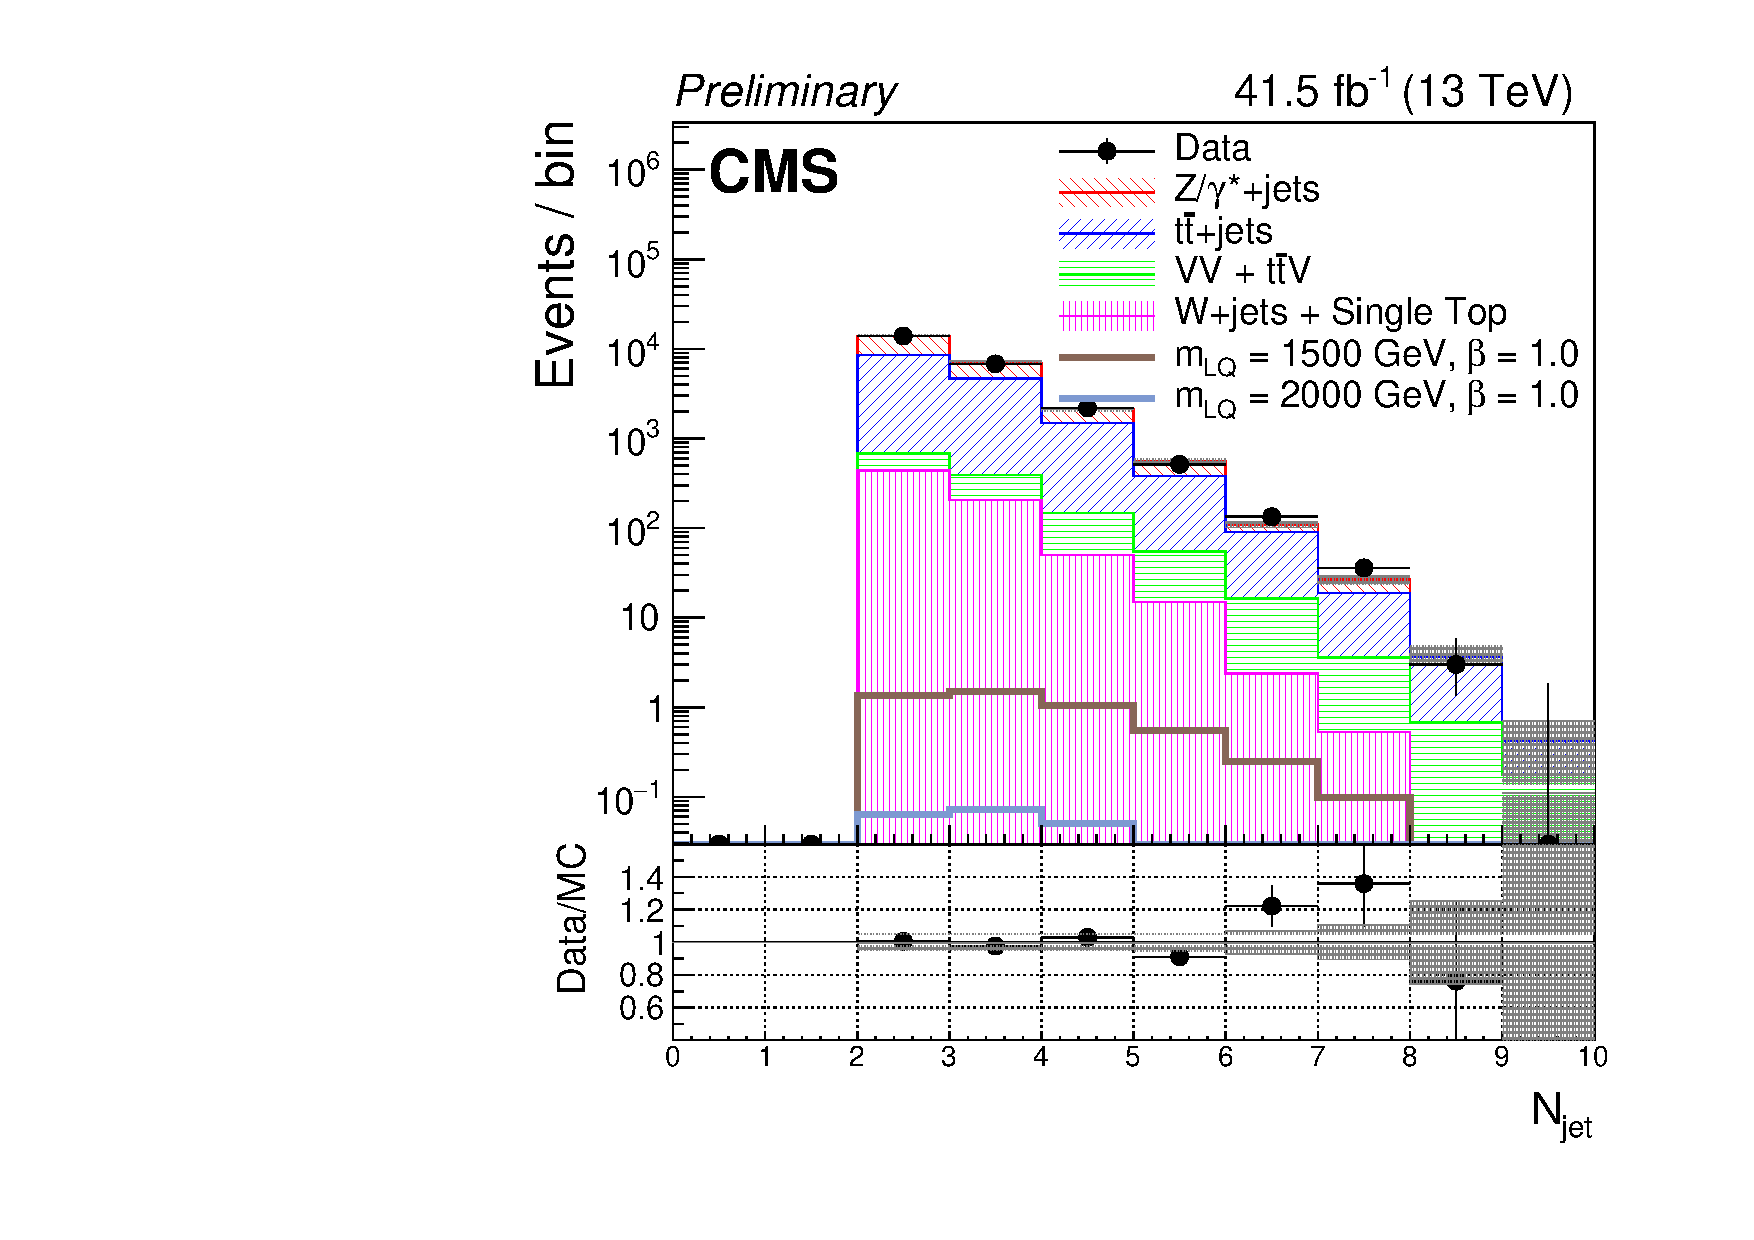
\includegraphics[width=.32\textwidth]{Images/Analysis/Results_2017_Unblinded/Plots/Preselection/BasicLQ_uujj_JetCount_standard.pdf}}
       {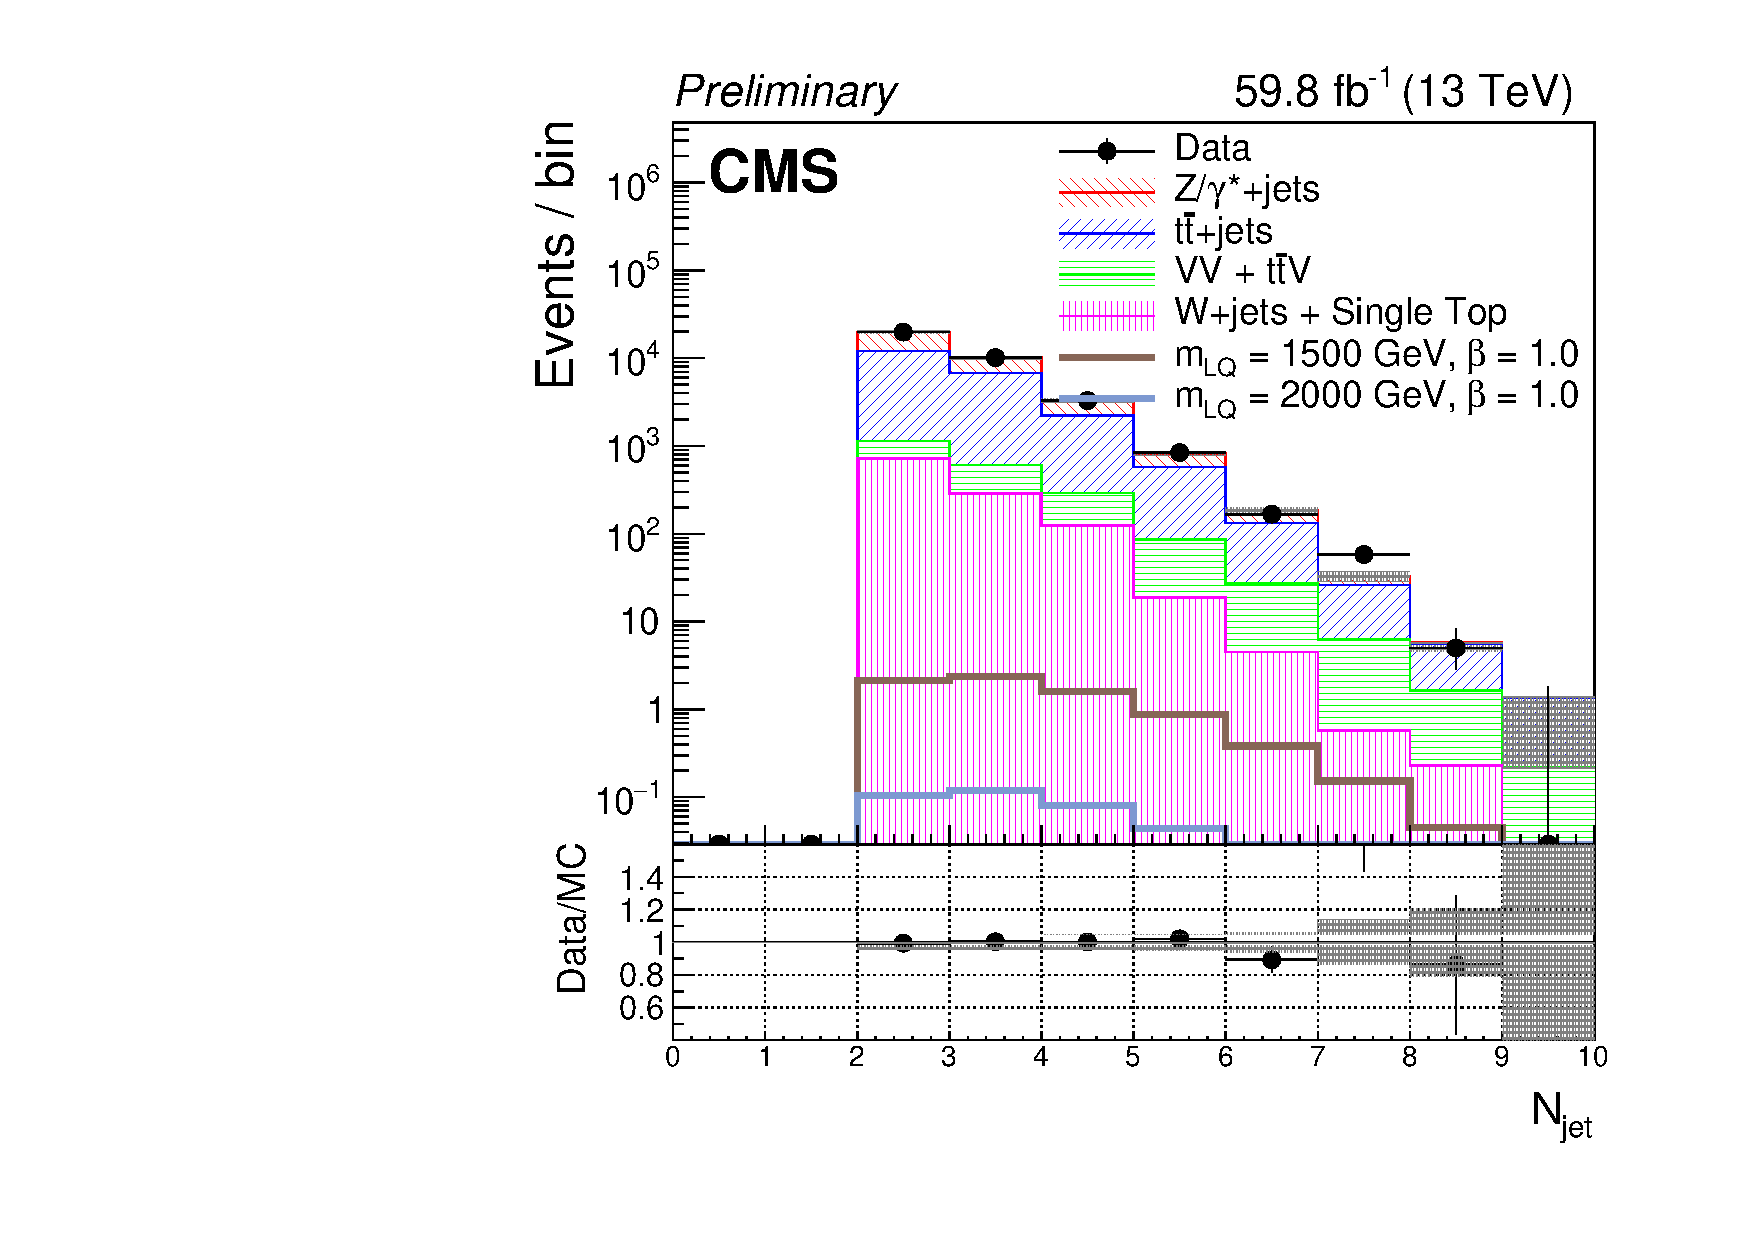
\includegraphics[width=.32\textwidth]{Images/Analysis/Results_2018_Unblinded/Plots/Preselection/BasicLQ_uujj_JetCount_standard.pdf}}
       {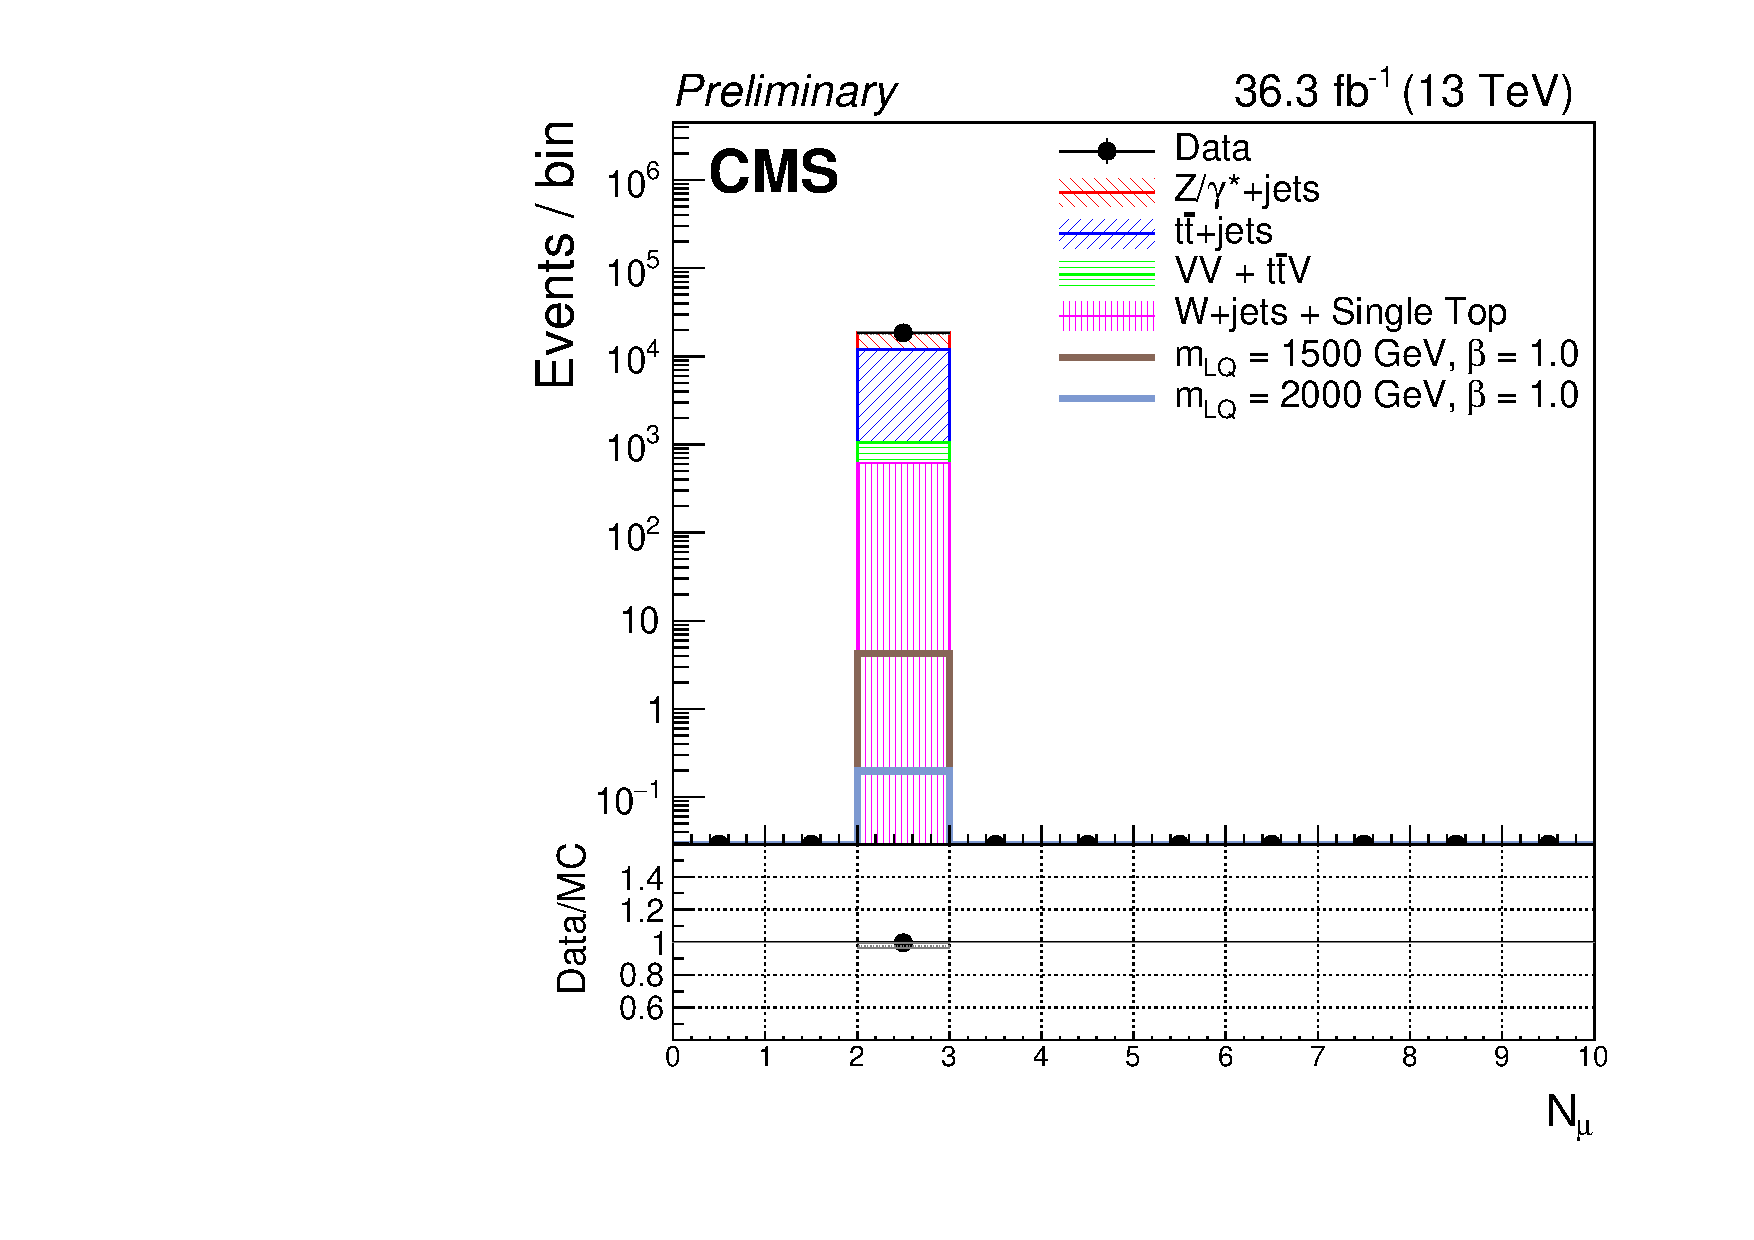
\includegraphics[width=.32\textwidth]{Images/Analysis/Results_2016_Unblinded/Plots/Preselection/BasicLQ_uujj_MuonCount_standard.pdf}}
       {\includegraphics[width=.32\textwidth]{Images/Analysis/Results_2017_Unblinded/Plots/Preselection/BasicLQ_uujj_MuonCount_standard.pdf}}
       {\includegraphics[width=.32\textwidth]{Images/Analysis/Results_2018_Unblinded/Plots/Preselection/BasicLQ_uujj_MuonCount_standard.pdf}}
       \caption{A comparison between distributions of observed data and SM expectation at preselection level. Left to right: 2016, 2017, 2018 data. Top to bottom: \ST, \ptmiss, jet multiplicity, and muon multiplicity. Error bars on observed data points represent statistical uncertainties, and systematic uncertainties on SM expectation are shown by gray hashing.}
    \label{figapp:preselmisc}
\end{figure}

\begin{figure}[H]
       \centering
       {\includegraphics[width=.32\textwidth]{Images/Analysis/Results_2016_Unblinded/Plots/Preselection/BasicLQ_uujj_M_uu_standard.pdf}}
       {\includegraphics[width=.32\textwidth]{Images/Analysis/Results_2017_Unblinded/Plots/Preselection/BasicLQ_uujj_M_uu_standard.pdf}}
       {\includegraphics[width=.32\textwidth]{Images/Analysis/Results_2018_Unblinded/Plots/Preselection/BasicLQ_uujj_M_uu_standard.pdf}}
       {\includegraphics[width=.32\textwidth]{Images/Analysis/Results_2016_Unblinded/Plots/Preselection/BasicLQ_uujj_M_uujj_standard.pdf}}
       {\includegraphics[width=.32\textwidth]{Images/Analysis/Results_2017_Unblinded/Plots/Preselection/BasicLQ_uujj_M_uujj_standard.pdf}}
       {\includegraphics[width=.32\textwidth]{Images/Analysis/Results_2018_Unblinded/Plots/Preselection/BasicLQ_uujj_M_uujj_standard.pdf}}
       {\includegraphics[width=.32\textwidth]{Images/Analysis/Results_2016_Unblinded/Plots/Preselection/BasicLQ_uujj_M_uujj1_standard.pdf}}
       {\includegraphics[width=.32\textwidth]{Images/Analysis/Results_2017_Unblinded/Plots/Preselection/BasicLQ_uujj_M_uujj1_standard.pdf}}
       {\includegraphics[width=.32\textwidth]{Images/Analysis/Results_2018_Unblinded/Plots/Preselection/BasicLQ_uujj_M_uujj1_standard.pdf}}
       {\includegraphics[width=.32\textwidth]{Images/Analysis/Results_2016_Unblinded/Plots/Preselection/BasicLQ_uujj_M_uujj2_standard.pdf}}
       {\includegraphics[width=.32\textwidth]{Images/Analysis/Results_2017_Unblinded/Plots/Preselection/BasicLQ_uujj_M_uujj2_standard.pdf}}
       {\includegraphics[width=.32\textwidth]{Images/Analysis/Results_2018_Unblinded/Plots/Preselection/BasicLQ_uujj_M_uujj2_standard.pdf}}
       \caption{A comparison between distributions of observed data and SM expectation at preselection level. Left to right: 2016, 2017, 2018 data. Top to bottom: \Muu, \Muujj, \MujOne, and \MujTwo. Error bars on observed data points represent statistical uncertainties, and systematic uncertainties on SM expectation are shown by gray hashing.}
       \label{figapp:preselmass}
\end{figure}


\begin{figure}[H]
       \centering
       {\includegraphics[width=.32\textwidth]{Images/Analysis/Results_2016_Unblinded/Plots/Preselection/BasicLQ_uujj_DeepJet_jet1_standard.pdf}}
       {\includegraphics[width=.32\textwidth]{Images/Analysis/Results_2017_Unblinded/Plots/Preselection/BasicLQ_uujj_DeepJet_jet1_standard.pdf}}
       {\includegraphics[width=.32\textwidth]{Images/Analysis/Results_2018_Unblinded/Plots/Preselection/BasicLQ_uujj_DeepJet_jet1_standard.pdf}}
       {\includegraphics[width=.32\textwidth]{Images/Analysis/Results_2016_Unblinded/Plots/Preselection/BasicLQ_uujj_DeepJet_jet2_standard.pdf}}
       {\includegraphics[width=.32\textwidth]{Images/Analysis/Results_2017_Unblinded/Plots/Preselection/BasicLQ_uujj_DeepJet_jet2_standard.pdf}}
       {\includegraphics[width=.32\textwidth]{Images/Analysis/Results_2018_Unblinded/Plots/Preselection/BasicLQ_uujj_DeepJet_jet2_standard.pdf}}
       \caption{A comparison between distributions of observed data and SM expectation at preselection level. Left to right: 2016, 2017, 2018 data. Top to bottom: DeepJet b tag score of jet 1 and DeepJet b tag score of jet 2. Error bars on observed data points represent statistical uncertainties, and systematic uncertainties on SM expectation are shown by gray hashing.}
    \label{figapp:preselbtag}
\end{figure}

% Combined plots here

\begin{figure}[H]
       \centering
       {\includegraphics[width=.49\textwidth]{Images/Analysis/Results_combined_Unblinded/Plots/Preselection/BasicLQ_uujj_GoodVertexCount_standard.pdf}}
       \caption{A comparison of the number of reconstructed vertices at preselection level in the combination of 2016, 2017, and 2018 data. Error bars shown represent statistical uncertainties, and systematic uncertainties are shown by gray hashing.}
       \label{fig:vertexCombined}
\end{figure}

\begin{figure}[H]
       \centering
       {\includegraphics[width=.49\textwidth]{Images/Analysis/Results_combined_Unblinded/Plots/Preselection/BasicLQ_uujj_Pt_muon1_standard.pdf}}
       {\includegraphics[width=.49\textwidth]{Images/Analysis/Results_combined_Unblinded/Plots/Preselection/BasicLQ_uujj_Pt_muon2_standard.pdf}}
       {\includegraphics[width=.49\textwidth]{Images/Analysis/Results_combined_Unblinded/Plots/Preselection/BasicLQ_uujj_Pt_jet1_standard.pdf}}
       {\includegraphics[width=.49\textwidth]{Images/Analysis/Results_combined_Unblinded/Plots/Preselection/BasicLQ_uujj_Pt_jet2_standard.pdf}}
       \caption{A comparison between distributions of observed data and SM expectation at preselection level in the combination of 2016, 2017, and 2018 data. Left to right, top to bottom: muon 1 \pt, muon 2 \pt, jet 1 \pt, and jet 2 \pt. Error bars on observed data points represent statistical uncertainties, and systematic uncertainties on SM expectation are shown by gray hashing.}
	\label{figa:preselptCombined}
\end{figure}

\begin{figure}[H]
       \centering
       {\includegraphics[width=0.49\textwidth]{Images/Analysis/Results_combined_Unblinded/Plots/Preselection/BasicLQ_uujj_DR_muon1jet1_standard.pdf}}
       {\includegraphics[width=0.49\textwidth]{Images/Analysis/Results_combined_Unblinded/Plots/Preselection/BasicLQ_uujj_DR_muon1jet2_standard.pdf}}
       {\includegraphics[width=0.49\textwidth]{Images/Analysis/Results_combined_Unblinded/Plots/Preselection/BasicLQ_uujj_DR_muon2jet1_standard.pdf}}
       {\includegraphics[width=0.49\textwidth]{Images/Analysis/Results_combined_Unblinded/Plots/Preselection/BasicLQ_uujj_DR_muon2jet2_standard.pdf}}
       \caption{A comparison between distributions of observed data and SM expectation at preselection level in the combination of 2016, 2017, and 2018 data. Left to right, top to bottom: \DR between muon 1 and jet 1, \DR between muon 1 and jet 2, \DR between muon 2 and jet 1, and \DR between muon 2 and jet 2. Error bars on observed data points represent statistical uncertainties, and systematic uncertainties on SM expectation are shown by gray hashing.}
       \label{fig:preseldrCombined}
\end{figure}

\begin{figure}[H]
       \centering
       {\includegraphics[width=.49\textwidth]{Images/Analysis/Results_combined_Unblinded/Plots/Preselection/BasicLQ_uujj_St_uujj_standard.pdf}}
       {\includegraphics[width=.49\textwidth]{Images/Analysis/Results_combined_Unblinded/Plots/Preselection/BasicLQ_uujj_Pt_miss_standard.pdf}}
       {\includegraphics[width=.49\textwidth]{Images/Analysis/Results_combined_Unblinded/Plots/Preselection/BasicLQ_uujj_JetCount_standard.pdf}}
       {\includegraphics[width=.49\textwidth]{Images/Analysis/Results_combined_Unblinded/Plots/Preselection/BasicLQ_uujj_MuonCount_standard.pdf}}
       \caption{A comparison between distributions of observed data and SM expectation at preselection level in the combination of 2016, 2017, and 2018 data. Left to right, top to bottom: \ST, \ptmiss, jet multiplicity, and muon multiplicity. Error bars on observed data points represent statistical uncertainties, and systematic uncertainties on SM expectation are shown by gray hashing.}
    \label{fig:preselmiscCombined}
\end{figure}

\begin{figure}[H]
       \centering
       {\includegraphics[width=.49\textwidth]{Images/Analysis/Results_combined_Unblinded/Plots/Preselection/BasicLQ_uujj_M_uu_standard.pdf}}
       {\includegraphics[width=.49\textwidth]{Images/Analysis/Results_combined_Unblinded/Plots/Preselection/BasicLQ_uujj_M_uujj_standard.pdf}}
       {\includegraphics[width=.49\textwidth]{Images/Analysis/Results_combined_Unblinded/Plots/Preselection/BasicLQ_uujj_M_uujj1_standard.pdf}}
       {\includegraphics[width=.49\textwidth]{Images/Analysis/Results_combined_Unblinded/Plots/Preselection/BasicLQ_uujj_M_uujj2_standard.pdf}}
       \caption{A comparison between distributions of observed data and SM expectation at preselection level in the combination of 2016, 2017, and 2018 data. Left to right, top to bottom: \Muu, \Muujj, \MujOne, and \MujTwo. Error bars on observed data points represent statistical uncertainties, and systematic uncertainties on SM expectation are shown by gray hashing.}
       \label{fig:preselmassCombined}
\end{figure}


\begin{figure}[H]
       \centering
       {\includegraphics[width=.49\textwidth]{Images/Analysis/Results_combined_Unblinded/Plots/Preselection/BasicLQ_uujj_DeepJet_jet1_standard.pdf}}
       {\includegraphics[width=.49\textwidth]{Images/Analysis/Results_combined_Unblinded/Plots/Preselection/BasicLQ_uujj_DeepJet_jet2_standard.pdf}}
       \caption{A comparison between distributions of observed data and SM expectation at preselection level in the combination of 2016, 2017, and 2018 data. Left to Right: DeepJet b tag score of jet 1 and DeepJet b tag score of jet 2. Error bars on observed data points represent statistical uncertainties, and systematic uncertainties on SM expectation are shown by gray hashing.}
    \label{fig:preselbtagCombined}
\end{figure}
